\documentclass[a4paper,14pt, ukrainian]{extarticle}
\usepackage[T1,T2A]{fontenc}
\usepackage[utf8]{inputenc} %useful to type directly diacritic characters
\usepackage[ukrainian]{babel}
\usepackage{graphicx} %Loading the package
\graphicspath{{images/}}
\usepackage[export]{adjustbox}
\usepackage{setspace}
\usepackage{mathtools}
\usepackage{float}
\usepackage{extsizes}

% \usepackage[utf8]{inputenc}
% \usepackage{mathptmx}




\usepackage[usenames]{color} %used for font color
\usepackage{amssymb} %maths
\usepackage{amsmath} %maths
\usepackage[dvipsnames]{xcolor}
\usepackage{bbm}
\numberwithin{equation}{section}
\usepackage{booktabs}
\usepackage[normalem]{ulem}
% \usepackage[nottoc,numbib]{tocbibind}
\usepackage{subcaption}
\usepackage{graphicx}
\usepackage{indentfirst} % отделять первую строку раздела абзацным отступом тоже
\usepackage{hyperref}
\usepackage{listings}
\usepackage{fancyhdr}
\usepackage{tocloft}
\usepackage{fancyhdr}
\usepackage{tempora}
\usepackage{titlesec}

\usepackage{geometry}
\usepackage{enumitem}


\pagestyle{fancy}
\fancyhf{}
\fancyhead[R]{\thepage}
\fancyheadoffset{0mm}
\fancyfootoffset{0mm}
\setlength{\headheight}{17pt}
\renewcommand{\headrulewidth}{0pt}
\renewcommand{\footrulewidth}{0pt}
\addto\captionsukrainian{\def\refname{ПЕРЕЛІК ДЖЕРЕЛ ПОСИЛАНЬ}}
\addto\captionsukrainian{\renewcommand{\figurename}{Рисунок}}
\fancypagestyle{plain}{ 
    \fancyhf{}
    \rhead{\thepage}}

\newcommand{\sectionbreak}{\clearpage} % Кожна сеекція із нової сторінки

\titleformat{\chapter}[display]
    {\filcenter}
    {\MakeUppercase{\chaptertitlename} \thechapter}
    {8pt}
    {\bfseries}{}
 
\titleformat{\section}
    {\centering\normalsize\bfseries}
    {\thesection}
    {1em}{}
 
\titleformat{\subsection}
    {\normalsize\bfseries}
    {\thesubsection}
    {1em}{}
 
\geometry{left=3cm}
\geometry{right=1.5cm}
\geometry{top=2cm}
\geometry{bottom=2cm}
% Настройка вертикальных и горизонтальных отступов
\titlespacing*{\chapter}{0pt}{-30pt}{8pt}
\titlespacing*{\section}{\parindent}{*4}{*4}
\titlespacing*{\subsection}{\parindent}{*4}{*4}

\makeatletter
    \AddEnumerateCounter{\asbuk}{\@asbuk}{м)}
\makeatother
\setlist{nolistsep}
\renewcommand{\labelitemi}{-}
% \renewcommand{\labelenumi}{\asbuk{enumi})}
\renewcommand{\labelenumii}{\arabic{enumii})}

\tocloftpagestyle{empty}
\addto\captionsukrainian{%
  \renewcommand{\contentsname}{ЗМІСТ}%
}
\renewcommand{\cfttoctitlefont}{\hspace{0.5\textwidth}\bfseries}
\renewcommand{\cftbeforetoctitleskip}{1em}
% \renewcommand{\cftaftertoctitle}{\mbox{}\hfill \\ \mbox{}\hfill{\footnotesize Стр.}\vspace{-2.5em}}
\renewcommand{\cftsecfont}{\bfseries\hspace{31pt}}
\renewcommand{\cftsubsecfont}{\hspace{14pt}}
\renewcommand{\cftparskip}{-1mm}
\renewcommand{\cftdotsep}{1}
\setcounter{tocdepth}{2} % задать глубину оглавления — до subsection включительно


\makeatletter
    \renewcommand{\@dotsep}{2}
    \newcommand{\l@likechapter}[2]{{\bfseries\@dottedtocline{0}{0pt}{0pt}{#1}{#2}}}
\makeatother

% \newcommand{\likechapter}[1]{    
%     \likechapterheading{#1}    
%     \addcontentsline{toc}{likechapter}{\MakeUppercase{#1}}}

\useunder{\uline}{\ul}{}
\DeclareRobustCommand{\[}{\begin{equation}}
\DeclareRobustCommand{\]}{\end{equation}}
\counterwithin{figure}{section}
\counterwithin{table}{section}

\renewcommand{\cftsubsecaftersnum}{} % що буде писатися після номеру пункта (нічого)
\renewcommand{\cftsubsecindent}{3em} % відступ номера пункта від лівого краю
\renewcommand{\cftsubsecnumwidth}{2.5em} % розмір поля, що виділяється під номер пункта
\renewcommand{\cftsubsecpagefont}{\mdseries} % стиль номеру сторінки (звичайний, 14pt)
\renewcommand{\cftsubsecfont}{\mdseries} % стиль заголовку (звичайний)
\renewcommand{\cftsubsecleader}{\cftdotfill{\cftsubsecdotsep}} % чим заповнювати проміжок від заголовку до номеру сторінки (точками)

\title{Оцінка якості моделей глибокого начання у системах рекомендацій}
\author{Володимир Малиняк}

\begin{document}

\section*{ПЕРЕЛІК УМОВНИХ ПОЗНАЧЕНЬ}
\addcontentsline{toc}{section}{ПЕРЕЛІК УМОВНИХ ПОЗНАЧЕНЬ}
    \begin{tabular}{|l|l|}
    \hline
    Скорочена назва & Повна назва                                                          \\ \hline
    MLP             & Multilayer Perceptron                                                \\ \hline
    RS              & Recommendation Systems                                               \\ \hline
    VAE             & Variational Auto Encoder                                             \\ \hline
    AE              & Auto Encoder                                                         \\ \hline
    NGCF            & Neural graph collaborative filtering                                 \\ \hline
    MSE             & Mean Square Error                                                    \\ \hline
    ML              & Machine Learning                                                     \\ \hline
    DL              & Deep Learning                                                        \\ \hline
    DNN             & Deep Neural Networks                                                 \\ \hline
    PCA             & Principal component analysis                                         \\ \hline
    GNN             & Graph Neural Networks                                                \\ \hline
    DCG             & \begin{tabular}[c]{@{}l@{}}Discounted Cumulative\\ Gain\end{tabular} \\ \hline
    NCF             & Neural Collaborative Filtering                                       \\ \hline
    EDA & Explorative Data Analysis \\ \hline
    \end{tabular}
\thispagestyle{empty}
\onehalfspacing
% \maketitlepage
\newpage
\tableofcontents
\section*{ВСТУП}
\addcontentsline{toc}{section}{ВСТУП}
\subsection*{Предмет дослідження}
Предметом дослідження є оцінка якості роботи алгоритмів побудови рекомендацій на основі глибокого навчання. 
\subsection*{Завдання дослідження}
Провести комплексний аналіз систем рекомендацій на основі моделей глибокого навчання. Дослідити ключові особливості алгоритмів рекомендацій на основі моделей глибокого навчання. Класифікувати і оцінити фактори впливу на якість роботи алгоритмів. Розробити стратегію для комплексної оцінки і порівняння алгоритмів рекомендацій на основі глибокого навчання. 
\subsection*{Актуальність дослідження}
Внаслідок розробки великої кількості нових рекомендаційних алгоритмів постало критичне питання у вітсутності єдиного підходу до оцінки їх еффективності, що призводитть до нерепродуктивних та несправедливих результів їх порівняння.
\newpage
\section{ОГЛЯД СУЧАСНОГО СТАНУ ОБЛАСТІ ПОБУДОВИ СИСТЕМ РЕКОМЕНДАЦІЙ}
У наслідок зривного росту сфери інформаційних технологій і стрімким пересіченням буденного життя звичайних людей із системами обміну данними відкриваються нові можливості для впливу на процеси прийняття рішень, таких як - який фільм переглянути, прослухати музику або яку річ купити. Крім того за останнє десятиліття користувачі стикаються із дилемою вибору серед великої кількості варіантів. Як результат, автоматичні рекомендації є важливими для покращення досвіду користувачів та зменшення перевантаження інформації. Загалом, системи рекомендацій відіграли незамінну роль у різних системах фільтрації інформації для підвищення цінності бізнесу та полегшення процесів прийняття рішень. Netfilx - типовий приклад системи рекомендацій (Рис. 1.1).

\begin{figure}[H]
    \centering
    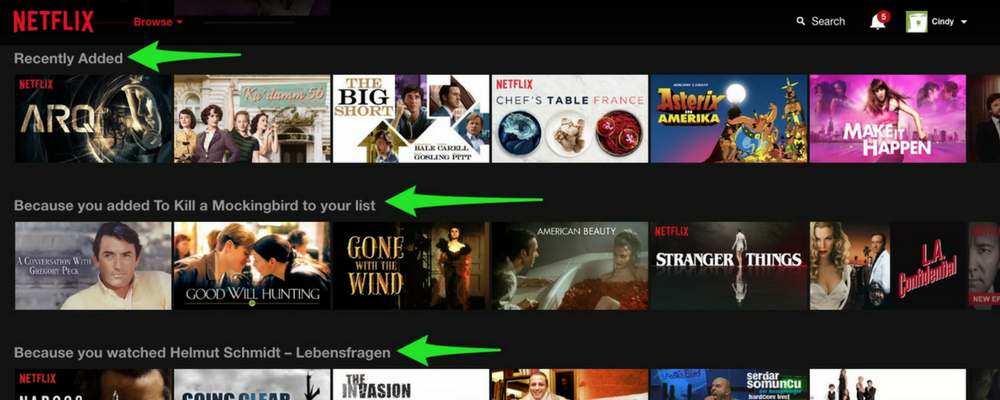
\includegraphics[width=1\textwidth]{images/netflixl.png}
    \caption{Інтерфейс головної сторінки стрімінгової платформи Netflix. }

\end{figure}

У своїй найпростішій формі персоналізовані рекомендації пропонуються як ранжовані списки елементів. Виконуючи це рейтингування, RS намагаються передбачити які продукти чи послуги є найбільш релевантними, виходячи з уподобань і обмежень користувача. Щоб виконати таке обчислювальне завдання, RS збирають інформацію від користувачів щодо їхніх уподобань, які або явно виражені, наприклад, як рейтинги для продуктів, або виводяться шляхом інтерпретації дій користувача. Наприклад, RS може розглядати навігацію до сторінки конкретного продукту як неявний знак переваги для елементів, показаних на цій сторінці.

В останні роки інтерес до рекомендаційних систем різко зріс, про це свідчать такі факти:
\begin{enumerate}
    \item Системи рекомендацій відіграють важливу роль на високорейтингових інтернет-сайтах, таких як Amazon.com, YouTube, Netflix, Spotify, LinkedIn, Facebook, Tripadvisor, та IMDb. Крім того, багато медіа-компаній зараз розробляють і розгортають RSs як частину послуг які вони надають своїм передплатникам. Наприклад, Netflix, онлайн-провайдер потокового мультимедіа, присудив приз у мільйон доларів команді, яка першою зуміла суттєво покращити продуктивність своєї системи рекомендацій.

    \item Активна робота введеться у наукові сфері. Популярні академічні журнали активно публікують результати досліджень у сфері систем рекомендацій. Існують різні методи проектування цих систем, починаючи від простого (наприклад, заснованого лише на номінальних елементах від одного користувача) до надзвичайно складного. Складні рекомендаційні системи використовують різноманітні джерела даних і часто використовують нелінійні методи навчання. Таким чином, завдання рекомендації забезпечує відмінний простір для застосування методологій машинного навчання. Оскільки користувачі продовжують споживати вміст і дають більше даних, ми можемо створити системи на основі машинного навчання для використання цих даних для надання кращих та кращих рекомендацій.
\end{enumerate}

\subsection{Призначення системи рекомендацій}
Система рекомендацій знайшла своє призначення у багатьох сферах виконуючи наступні завдання:
\begin{itemize}
    \item Збільшення кількості проданого товару. З точки зору бізнесу, збільшення конвертацій (співвідношення кількості переглядів до цільових дій - покупки, продажу, перегляду і т.д.) є головною метою.
    \item Збільшення різноманітності (diversity) проданого товару. Тобто реалізація непопулярного товару без ризику втратити прихильність користувачів
    \item Збільшення задоволеності користувачів. Добре розроблена система рекомендацій може покращити досвід користувачів у програмі. Користувач вважатиме рекомендації цікавими, актуальними та приємними. Це призводить до більш високого загального задоволення.
    \item Зрозуміти потреби користувача. Хороша система рекомендацій детально описує бажання користувачів, явно або неявно. Тоді бізнес може вирішити повторно використовувати ці знання для багатьох інших цілей.
\end{itemize}
\subsection{Прикладні сфери використання}

Дослідження рекомендаційних систем, як правило, проводяться з сильним акцентом на практичні та комерційні програми. Домен застосування суттєво впливає на тип алгоритмічного підходу, який слід застосовувати. Умовно можна надати таку таксономію систем рекомендацій що класифікує існуючі програми до конкретних доменів:
\begin{itemize}
    \item  Розваги - Рекомендації щодо фільмів (Netflix), Музика (Spotify, Pandora) та мобільних додатків (Apple Store, Android Store).
    \item Соціальні мережі.
    \item Вміст-персоналізовані газети (The New York Times, The Wall Street Journal), рекомендація щодо зображень (Pinterest), рекомендації веб-сторінок, електронного навчання (Coursera) та електронних листів (Gmail).
    \item Електронна комерція - Рекомендації для споживачів продуктів для придбання, таких як книги (Amazon), косметика, одяг та багато іншого.
    \item Рекомендації туристичних послуг (Skyscanner), експертів з консультацій (Styleseat, ClassPass), будинки для оренди (AirBnB) або послуги із пошуку партнера (Tinder, Bumble).
\end{itemize}

\subsection{Проблематика напрямку}
Хоча завдання створення автоматичної рекомендації не є новим, залишається багато проблем які сприяють дослідженням сучасних систем, особливо у задачах колаборативної фільтрації, які мають на меті змоделювати поведінку користувачів для полегшення рекомендацій. Основі питання:
\begin{itemize}
    \item Розрідженість (Data sparsity): Проблема розрідження є досить помітною у системах колаборативної фільтрації, оскільки лише невелика кількість користувачів надає рейтинги, і лише невелика кількість предметів має достатню кількість оцінок. Це явище відоме як "проблема холодного старту" (сold start problem), що запобігає системі рекомендацій генерувати змістовні прогнози для нових користувачів через обмеженість даних.
    \item Надмірна спеціалізованісь (Over specialized): Система рекомендує об’єкти дуже схожі до тих які вже відомі користувачу. Незважаючи на те, що це свідчить про хороший загальний рівень прогнозувань моделі (її ефективність), система не привносить різноманіття, відкриття нового, не знайомого контенту.
    \item Упередження на основі популярності (Popularity bias | "Harry Potter Effect"): Частково проблема систем колаборативної фільтрації. Через нерівномірність матриці взаємодій алгоритм рекомендує об’єкти із великою кількістю оцінок (відгуків), а при  недостатній кількості обє’кти ігноруються.
    \item Точність: Системи рекомендацій повинні забезпечити високий рівень точності прогнозування, щоб забезпечити якість, яку користувачі часто вимагають. У дослідженні точність зазвичай оцінюється/досліджується шляхом прогнозування рейтингу та рейтингу предметів.
    \item Маштабованість: Системи рекомендацій у реальному світі розгортаються в динамічному і інтерактивному середовищі - дані користувачів та елементів швидко надходять і виходять. Важливо вирішити обчислювальні вимоги та час навчання/виведення, необхідні для ефективної обробки цих даних.
    \item Шахрайство.
          У рекомендаційних системах, де кожен може ставити оцінки, люди можуть давати позитивні оцінки своїм предметам і погані своїм конкурентам. Також, рекомендаційні системи стали сильно впливати на продажі та прибуток, з тих пір як отримали широке застосування в комерційних сайтах. Це призводить до того, що недобросовісні постачальники намагаються шахрайським чином піднімати рейтинг своїх продуктів і знижувати рейтинг свої конкурентів.

    \item Різноманітність.
          Колаборативна фільтрація спочатку визнана збільшити різноманітність, щоб дозволяти відкривати користувачам нові продукти з незліченної множини. Однак деякі алгоритми, зокрема основні на продажах і рейтингах, створюють дуже складні умови для просування нових і маловідомих продуктів, так як їх заміщають популярні продукти, які давно перебувають на ринку. Це в свою чергу тільки збільшує ефект «багаті стають ще багатшими» і приводить до меншої різноманітності.

    \item Білі ворони.
          До «білих ворон» відносяться користувачі, чия думка постійно не збігається з більшістю інших. Через унікальність смаку їм неможливо щось рекомендувати. Однак, такі люди мають проблеми з отриманням рекомендацій і в реальному житті, тому пошуки вирішення даної проблеми в даний час не ведуться.

    \item Проблема холодного старту.
          Нові предмети або користувачі представляють велику проблему для рекомендаційних систем. Частково проблему допомагає вирішити підхід, заснований на аналізі вмісту, так як він покладається не на оцінки, а на атрибути, що допомагає включати нові предмети в рекомендації для користувачів. Однак проблему з наданням рекомендації для нового користувача вирішити складніше.

    \item Синонімія.
          Синонімією називається тенденція схожих і однакових предметів мати різні імена. Більшість рекомендаційних систем не здатні виявити ці приховані зв'язки і тому відносяться до цих предметів як до різних. Наприклад, «фільми для дітей» та «дитячий фільм» відносяться до одного жанру, але система сприймає їх як різні.

    \item Розрідженість даних.
          Як правило, більшість комерційних рекомендаційних систем заснована на великій кількості даних (товарів), в той час як більшість користувачів не ставить оцінки товарам. В результаті цього матриця «предмет-користувач» виходить дуже великою і розрідженою, що представляє проблеми при обчисленні рекомендацій. Ця проблема особливо гостра для нових, щойно створених систем. Також розрідженість даних підсилює проблему холодного старту.
\end{itemize}

\subsection{Класифікація систем рекомендацій}
Існує два способи екстраполяції рейтингу від відомих об’єктів до невідомих.
Перший полягає у створені евристики, яка визначається функцією подібності та емпірично підтверджує ефективність. Друга навчається використовуючи функцію втрат, наприклад MSE або сross-entropy loss. Отримавши оцінку рейтингу для об’єктів рекомендацій ми рекомендуємо top n елементів із найвищим рейтингом.
Тому загальна класифікація систем рекомендацій наступна (Рис 1.2):
\begin{itemize}
    \item Фільтрування на основі контенту: система рекомендує нові елементи із характеристиками подібними до існуючих елементів, яким користувач віддав перевагу в минулому. Отже, генерація рекомендацій повністю залежить від історії взаємодій із елементами.
    \item Колаборативна фільтрація: система рекомендує об’єкти новим користувачам зі смаками схожими до існуючих користувачів у базі даних.Отже, якість рекомендацій залежить від уподобань користувача.
    \item Гібридний підхід: гібридна система поєднує фільтрацію на основі вмісту та колаборативну фільтрацію для створення рекомендацій.
\end{itemize}
\begin{figure}
    \centering
    
\includegraphics[width=1\textwidth]{images/Rec_system_types.png}
    \caption{Поділ систем рекомендацій за категоріями}
\end{figure}
\subsubsection{Фільтрування на основі вмісту}
У системах рекомендацій на основі вмісту функція корисності
$F(u,i)$ елемента $i$ для користувача $u$ оцінюється на основі
функцій $f(u,i_{k})$, призначеного користувачем $u$ для кожного
елемента $i_{k} \in I$, схожий на предмет $i$. Наприклад, у системі
рекомендацій музики, щоб рекомендувати нові пісні користувачеві
$U$,підхід до рекомендацій на основі вмісту намагається зрозуміти
подібність між піснями, які користувач u часто слухав у минулому.
Тоді лише пісні, які мають високу ступінь подібності з будь-якими
уподобаннями користувача, згодом рекомендуються.
Основні обмеження систем рекомендацій на основі вмісту:
\begin{enumerate}
    \item Обмежений аналіз: підходи на основі контенту обмежені функціями, які явно пов'язані з рекомендованими елементами. Отже, щоб мати можливість дати оцінку схожості, вміст повинен бути:
          \begin{enumerate}
              \item У форматі, який можна обробити автоматично
              \item Або може бути призначений елементам вручну.
          \end{enumerate}
          У першому сценарії створитти функції оцінки схожості в неструктурованих даних непросто, такі як зображення та аудіо. У другому сценарії часто недоцільно призначати атрибути вручну через обмежені обчислювальні та людські ресурси.
    \item Гомогенність: Коли система може рекомендувати лише елементи, які високо оцінюють профіль користувача, користувач обмежується лише предметами, подібними до тих, що вже оцінені. Іншими словами, підходи, засновані на контенті, не дають різноманітних рекомендацій. В ідеалі користувачеві слід представити широкий спектр варіантів, а не просто однорідний набір альтернатив.
    \item Рекомендації для нового користувача: Користувач повинен оцінити достатню кількість предметів до того, як система рекомендацій на основі вмісту може зрозуміти його/її вподобання та представити його/їй довірливими предметами. Таким чином, новий користувач, який не має попередніх рейтингів, не отримає точних рекомендацій
\end{enumerate}
\subsubsection{Колаборативна фільтрація}

У системах колаборативної фільтрації ми намагаємось передбачити корисність елементів для певного користувача на основі елементів, раніше оцінених іншими користувачами. Тобто, функція корисності $F(u, i)$ елемента $I$ для користувача $U$ оцінюється на основі функцій $F(u_{j}
    , i)$, призначеного елементу $I$ тими користувачами $u_{j} \in U$, які схожі на користувача $u$. Наприклад, у контексті програми рекомендацій щодо книги, щоб рекомендувати книги користувачеві $U$, система спільної фільтрації спочатку знаходить «однодумців» користувача $U$ або інших користувачів із подібними смаками в книгах (які оцінюють однакові книги аналогічно). Тоді, рекомендується лише книги, які найбільше подобаються похожим користувачам.

Алгоритми колаборативної фільтрації можна розділити на два основні класи: на основі сусідства та на основі моделі.

\subsubsection{Підхід оснований на сусідстві}
Алгоритм, заснований на сусідстві, обчислює подібність двох користувачів або виробів, виробляє прогноз для користувача, приймаючи середнє зважене всіх оцінок. Обчислення схожості між виробами або користувачами є важливою частиною цього підходу. Багаторазові заходи, такі як кореляції Пірсона і схожість, заснована на скалярному добутку, використовується для цього.

Схожість двох користувачів X, Y через кореляцію Пірсона визначається як:
\[simm(x,y) = \frac{{}\sum_{i \in I_{xy}}(r_{x,i} - \overline{r}_{x})(r_{y,i} - \overline{r}_{y})}
    {\sqrt{\sum_{i \in I} (r_{x,i} - \overline{r}_{x})^2(r_{y,i} - \overline{r}_{y})^2}}\] - де  $I_{x,y}$ набір елементів оцінений як користувачем x так і користувачем y.

Заснований на користувачеві алгоритм top-N рекомендації використовує засновану на подібності векторну модель для визначення K — більшості подібних користувачів до активного користувача. Після того, як знайдені найбільш схожі користувачі, їх відповідні матриці агрегуються для визначення рекомендованого набору елементів. Популярний метод, знаходження схожих користувачів — Locality-sensitive hashing, який реалізує механізм пошуку найближчих сусідів у лінійному часі.

Переваги цього підходу включають в себе: очікуваність результатів, що є важливим аспектом рекомендаційних систем; просте створення і використання; просте полегшення нових даних; добра масштабованість зі співавторами рейтингових пунктів.

Є також кілька недоліків при такому підході. Його продуктивність знижується, коли дані становляться розрідженими, що трапляється часто з виробами, пов'язаними з мережею. Це ускладнює масштабованість такого підходу і створює проблеми з великими наборами даних. Хоча він може ефективно обробляти нових користувачів, тому що спирається на структури даних, додавання нових елементів стає більш складним, що, як правило, спирається уявленням про конкретну складову векторного простору. Додавання нових елементів вимагає включення нового пункту і повторного включення всіх елементів у структурі.

\subsubsection{Підхід заснований на моделі}

Даний підхід надає рекомендації, вимірюючи параметри статистичних моделей для оцінок користувачів, побудованих за допомогою таких методів як, метод баєсовских мереж, кластеризації, латентно-семантичної моделі , такі як сингулярний розклад, імовірнісний латентно-семантичний аналіз, прихований розподіл Дирихле і марковський процес вирішування на основі моделей. Моделі розробляються з використанням інтелектуального аналізу даних, алгоритмів машинного навчання, щоб знайти закономірності на основі навчальних даних. Число параметрів в моделі може бути зменшено в залежності від типу за допомогою методу головних компонент.

Цей підхід є більш комплексним і дає більш точні прогнози, оскільки допомагає розкрити латентні фактори, що пояснюють спостережувані оцінки.

Даний підхід має ряд переваг. Він обробляє розріджені матриці краще, ніж підхід заснований на сусідстві, що в свою чергу допомагає з масштабністю великих наборів даних.

Недоліки цього підходу полягають в «дорогому» створенні моделі. Необхідний компроміс між точністю і розміром моделі, тому що можна втратити корисну інформацію у зв'язку із скороченням моделей.

Алгоритми на основі пам'яті-це евристика, яка прогнозує рейтинги на основі всієї колекції раніше оцінених елементів користувачами системи.
Алгоритми на основі моделі використовують колекцію рейтингів для навчання моделі (ML), які після валідації потім використовуються для прогнозування рейтингів.
% Колаборативні системи також мають особливі обмеження:
% \begin{enumerate}
%     \item Cold Start User: Це та сама проблема, що і у підходів, що базуються на Contentbaste. Щоб зробити точні рекомендації, система повинна спочатку вивчити переваги користувача з попередніх рейтингів.
%     \item Cold Start Item: Оскільки підходи спільної фільтрації покладаються виключно на переваги користувачів для надання рекомендацій, новий елемент не буде рекомендовано, поки він не буде оцінений достатньою кількістю користувачів.
%     \item Обмеженність (Data Sparsity): У будь -якій системі кількість вже отриманих оцінок зазвичай невелика порівняно з кількістю рейтингів, які потрібно прогнозувати. Ефективне прогнозування оцінок з невеликої кількості прикладів є досить важливим. Крім того, успіх спільної фільтрації залежить від наявності критичної маси користувачів. Наприклад, може бути багато продуктів, придбаних лише кількома людьми в системі рекомендацій щодо продуктів, а це означає, що вони були б рекомендовані дуже рідко, навіть якщо ці кілька користувачів дали ці товари високі рейтинги. Крім того, для користувача, чиї смаки незвичні порівняно з рештою населення, не буде жодних інших суттєво подібних користувачів, що дає погані рекомендації.
% \end{enumerate}

\subsubsection{Гібридні системи}
Даний підхід об'єднує в собі підхід заснований на сусідстві і заснований на моделі. Гібридний підхід є найпоширенішим при розробці рекомендаційних систем для комерційних сайтів, так як він допомагає подолати обмеження початкового оригінального підходу (заснованого на сусідстві) і поліпшити якість прогнозів. Цей підхід також дозволяє подолати проблему розрідженості даних і втрати інформації. Однак даний підхід складний і дорогий у реалізації та застосуванні.

\subsection{Постановка задачі системи рекомендацій}

У рекомендаційних системах релевантність об’єкта зазвичай представлена рейтингом, що вказує наскільки конкретному користувачеві подобається певний елемент. Корисність може бути довільною функцією і залежати від завдання.
Наприклад, елемент буде кориснішим, якщо він збільшує задоволення користувачів або краще підкріплює потреби користувача. Залежно від постановки, оцінка F може бути вказана користувачем - explicit feedback(як це часто робиться в контексті заповнених користувачами рейтингів), або обчислюється програмно - implicit feedback (значення бінаризовані, приймають 0 або 1).

Зважаючи на релевантність, строго, проблема рекомендації може бути сформульована таким чином:
\begin{itemize}
    \item Нехай $U$ будете набором всіх користувачів і нехай $I$ буде набором усіх елементів. Обидва ці простори можуть бути дуже великими - аж до потенційно мільйонів предметів.
    \item Нехай $F$ - функція важливості (корисності), яка вимірює відповідність елемента $i$ до користувача $u$ наступним чином: $f: U \times I \rightarrow R$,  де $R$ - це упорядкований набір налаштувань користувачів для елементів.
    \item Для кожного користувача $u \in U$ ми хочемо вибрати елемент $i \in I$, який максимально збільшує задоволеність користувача.
\end{itemize}

Тобто, ми хочимо вирішити наступну задачу оптимізації:
\[\forall u \in U, i_{s} = arg max_{i \in I}F(u,i)\]
де кожен елемент із простору користувачів U можна визначити за допомогою профілю, який включає різні характеристики, такі як ідентифікатор користувача, вік, стать, дохід тощо.
Аналогічно, кожен елемент простору елемента I визначається за допомогою (зокрема) набору характеристик. Наприклад, у завданнях музичної рекомендації -  Spotify, SoundCloud, Pandora, де I є колекцією пісень, кожна пісня може бути представлена не лише за її ідентифікатором, але і за назвою, жанром, виконавцем, роком випуску тощо.

Центральна проблема, з якою стикається будь-яка система рекомендацій, полягає в тому, що функція F зазвичай не визначається у всьому просторі $U \times I$ - вона, в кращому випадку, визначається лише на підмножині цього простору. Це означає, що F потрібно екстраполювати на весь простір $U \times I$.
У системах рекомендацій, функція F зазвичай представлена рейтингом і спочатку визначається лише на елементах, які раніше оцінювали (існуючі) користувачі. Наприклад, у програмі рекомендацій книг, як PlayBooks, користувачі спочатку оцінюють деяку підмножину книг, які вони вже читали. Мета програми - передбачити рейтинг до книг які не відомі користувачу, та відобразити відповідні рекомендації на основі цих прогнозів.

\subsection*{Висновок}
У розділі розглянуто постановку задачі системи рекомендацій. Наведено типові сфери використання, користь бізнесу і цілі. На основі розглянутої літератури було розглянуто класифікацію систем відносно підходу до побудови рекомендацій.
Проаналізовано проблематику напрямку.
\section{ПІДХІД ГЛИБОКОГО НАВЧАННЯ У ПОБУДОВІ РЕКОМЕНДАЦІЙ}
Моделі і алгоритми глибокого навчання на основі штучних нейронних мереж в останні роки знаходять своє використання у багатьох прикладних сферах інформатики. Цей підхід також показав прекрасні результати у порівнянні із класичними моделями у задачах побудови рекомендацій,що є наслідком уміння нейромереж знаходитити не лінійні і не тривіальні зв’язки у навчальних даних. А також, можливість використання в якості джерела даних як візуальну, так і текстову, контекстну інформацію. Розглянемо класичну структуру нейронної мережі.


\subsection{Нейронна мережа прямого поширення}
Перцептрон - математична модель яка відтворює сприйняття інформації за подобою мозку людини.Елементарний перцептрон складається з трьох типів елементів: S-елементів, А-елементів та одного R-елемента (Рис 3.1). S - це шар датчиків або рецепторів. У фізичному варіанті вони відповідають, наприклад, до схожих чутливих клітин сітківки ока або фоторезисторів матриці фотокамери. Кожен рецептор може бути в одному з двох станів - спокою або збудження, і лише в останньому випадку він передає сигнал до наступного шару і іншим  повязаним елементам.
\begin{figure}[H]
    \centering
    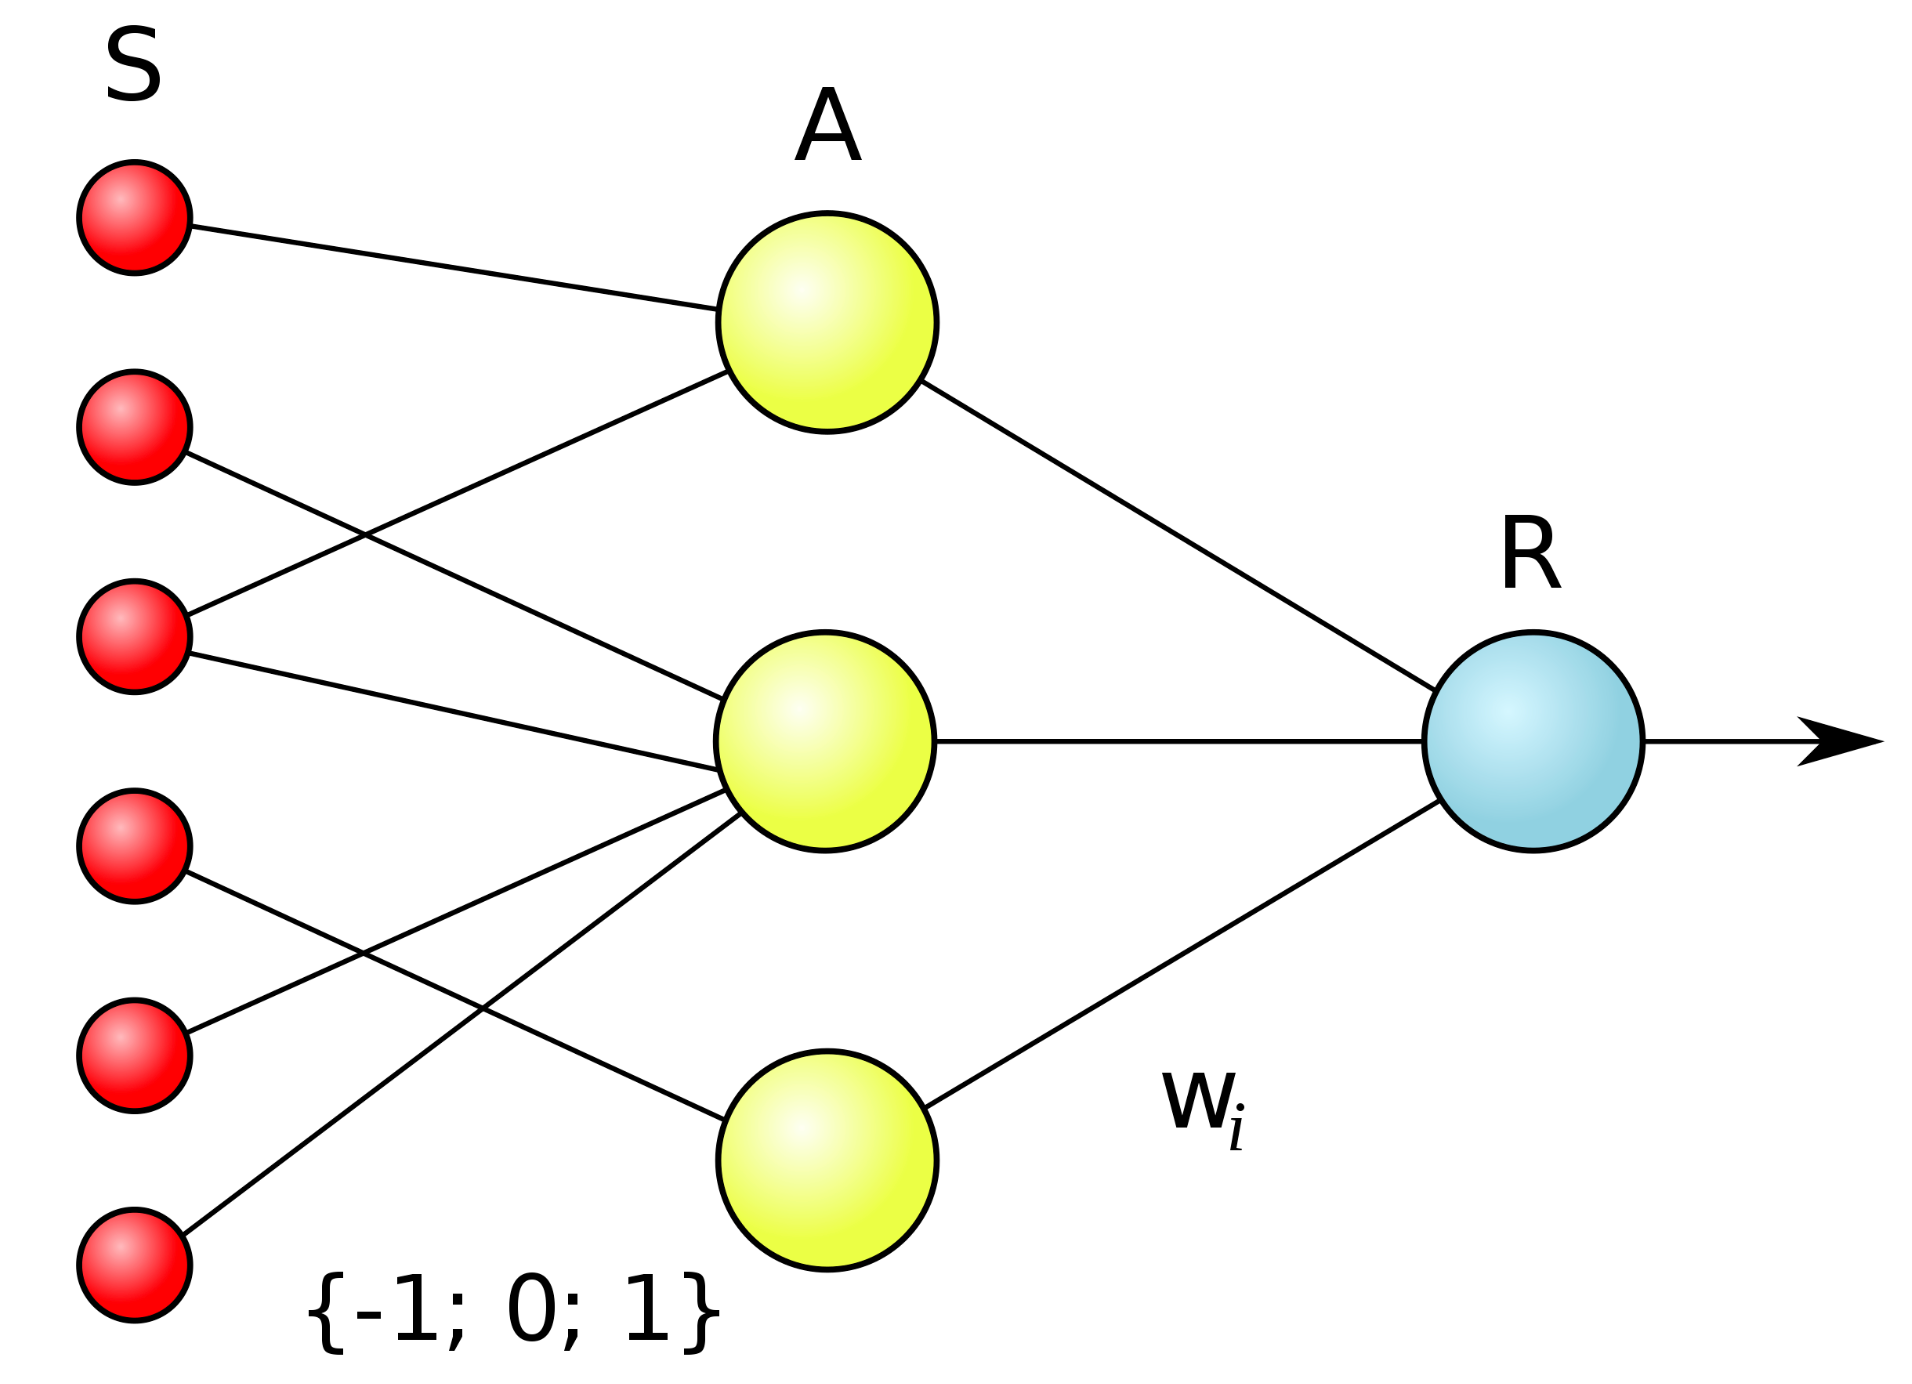
\includegraphics[width=0.6\textwidth]{images/LogicalPerceptron.png}
    \caption{Логічна схема елементарного перспетрону.}
\end{figure}
А-елементи називаються асоціативними, оскільки кожен такий елемент, як правило, відповідає цілому набору (асоціацій) S-елементів. А-елемент активується, як тільки кількість сигналів від S-елементів на його вході перевищила певне значення $\theta$.

Сигнали від збуджених А-елементів, у свою чергу, передаються на суматор R, кожен сигнал із i-того елемента передається із коефіцієнтом $ w_{i}$. Цей коефіцієнт називається вагою зв'язків A-R.

R-елемент обчислює суму значень вхідних сигналів, помножених на вагу (лінійна форма). R-елемент, а разом з ним і елементарний перцептрон, видає $1$, якщо сума перевищує поріг.

Навчання елементарного перцептрона полягає у зміні коефіцієнтів ваг $w_i$  звя’зків A-R. Ваги з'єднань S-A (які можуть приймати значення $[-1; 0; +1]$) та значення порогів A-елементів вибираються випадковим чином на самому початку, а потім не змінюють.

Багатошарова нейронна мережа - це нейронна мережа, що складається з вхідного шару, виходу та розташованих прихованих шарів нейронів (Рис. 3.2).
Такі мережі мають значно більші можливості, ніж персептрон, однак методи навчання нейронів прихованого шару були розроблені порівняно недавно.

Розглянемо це перетворення на прикладі лінійної регресії. Візьмемо $ X $ за вхідний вектор, зміщення $b$, вектор вагів $W$ і оцінку виходу $\hat{y}$.
\[\hat{y}=b + W^{T}X\]


Мінімізуючи функцію втрати, наприклад, MSE ми шукаємо оптимальне рішення.По мірі навчання будее зменшуватись різниця між нашою оцінкою $\hat{y}$ та реальним значенням $y$. Іншими словами, неоптимальні параметри призводять до більших втрат, ніж оптимальні параметри. У нейронній мережі прямого поширення ми використовуємо деяку функцію активації $a$:
\[\hat{y}=a(b + W^{T}X)\]
\begin{figure}
    \centering
    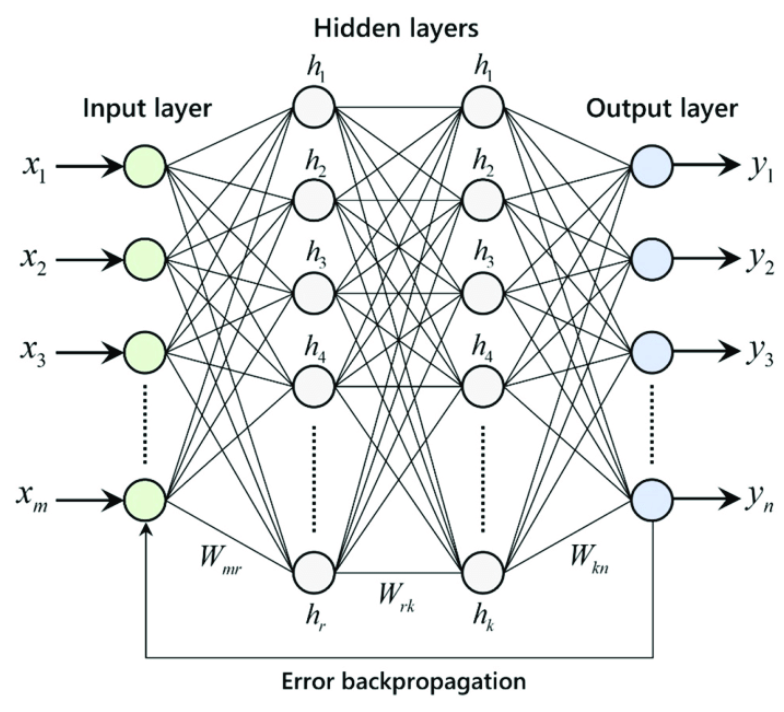
\includegraphics[width=0.4\textwidth]{images/MNN.png}
    \caption{Багатошарова нейронна мережа}
\end{figure}
Нелінійність надає моделі більшу гнучкість, шукаючи глобальний оптимум. Для еффективної роботи моделі нам потрібні ітераційні методи оптимізації.

Одним із найефективніших методів на сьогоднішній день є градієнтний спуск.
Глибокі нейронні мережі (DNN) зазвичай виконують міні-пакетний стохастичний спуск. Цей метод розбиває повну партію тренувань на частини (спліти), які збільшують частоту оновлення порівняно із навчанням на усіх даних (усіма навчальними зразками).

Алгоритим складається із прямого(forward propagation) і зворотнього проходу(backward propagation). На зворотньому проході ми оновлюємо наші параметри (ваги і зміщення) пропорційно обраному коефіцієнту $\alpha$.

\subsection{Автоенкодер}

Генеративні моделі знайшли своє використання у задачах
комп’ютерного зору та обробки природної мови.

Але останні дослідження показали що їх використання не обмежується тільки вищезгаданими сферами. У контексті побудови рекомендацій автоенкодери знайшли рішення групі важливих завдань.

До побудови рекомендацій можливо підійти як до завдання великих даних,внаслідок надзвичайно великого обє’му даних які генерються користувачами (так званий інформаційний слід). Але, із іншої сторони, ці дані в більшості випадків є ненасичені (користувачі взаємодіють лише із мізерною кількістю об’єктів). Що ускладнює завдання вивчення і передбачування побажань усіх користувачів. Для того щоб еффективно інтерпритувати розріджені сигнали було представлено ймовірносну модель засновану на Баєсовій статистиці яка здатна навчатись і поширюватись на скудно насичених даних.

\begin{figure}
    \centering
    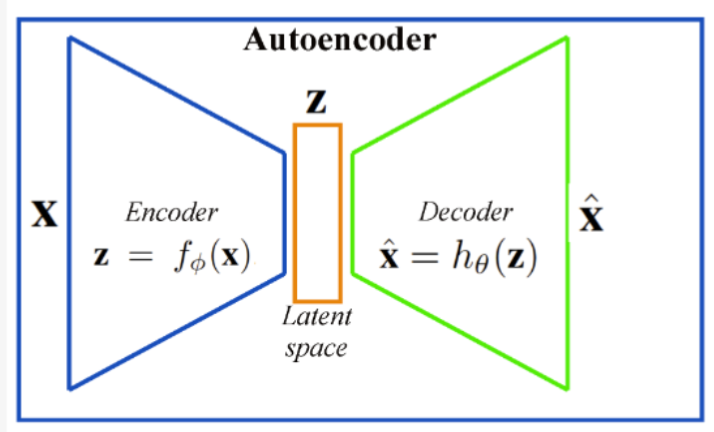
\includegraphics[width=0.7\textwidth]{images/Autoencoder.png}
    \caption{Архітектура нейронної мережі автоенкодера.}
\end{figure}
Автоенкодер у своєму класичному виді - це група із двох моделей глибоких нейронних мереж які використовуються для задачі кодування і декодування вхідних даних (Рис. 3.2).
Це кодування можна сприймати як один із способів зниження розмірності і комплексності вхідного датасету. Що, спрощує структуру моделей і полегшує швидкість навчання череез меншу кількість гіперпараметрів. Для низькорівневого умовного прикладу автоенкодера можна використати  алгоритм аналізу головних компонент (PCA). Ідея якого, це побудова нових признаків більш низької розмірності на основі лінійних комбінацій векторів базавого набору. Під час пошуку найкращої лінійної підмножини алгоритм мінімізує втрати інформації (Рис 3.3).


Але алгоритми такого класу суттєво обмежуються вимогами до не лінійності навчального набору, якщо дані лінійно не залежні алгоритм не знайде їх відображення - тому що його банально не існує.
\begin{figure}
    \centering
    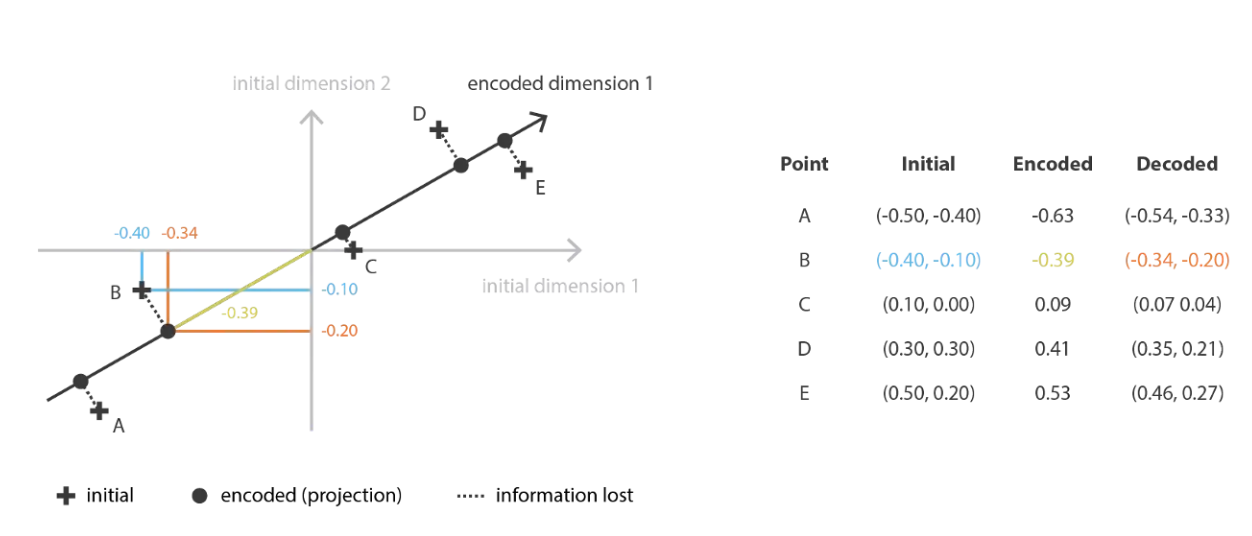
\includegraphics[width=1\textwidth]{images/PCA.png}
    \caption{PCA шукає найкраще відображення вхідних даних у лінійний підпростір меншого розміру}
\end{figure}
Внаслідок чого, були створені алгоритми де у якості енкодера і декодера використовуютсья нейронні мережі для пошуку найкращої функції ітераційним процесом оптимізації. Такий підхід також дозволяє не тільки ефективно кодувати простір, а і зберегти під час стискуваня важливу структурну інформацію.

Завдання навчання автоенкодера у класичному виді можна поставити наступним чином. Нехай $\mathbb{X} \in \mathbb{R}^{m}$ і $\mathbb{Z}\in \mathbb{R}^{n}$ є множини декодованих і закодованих об’єктів відповідно. А $E_{\phi}: \mathcal{X} \to \mathcal{Z} $ і $\mathcal{D}_{\theta}: \mathcal{Z} \to \mathcal{X}   $ деякі сімейства функцій енкодера і декодера пареметризовані $\phi$ і $\theta$ відповідно. Кожен $x \in \mathcal{X}$ вважається закодованим об’єктом при ${z}=\mathbb{E}_{\phi}(x)$ і декодованим (відновленим) при $z \in \mathcal{Z}, x^{\prime} = \mathbb{D}_{\theta}({z})$.

Також введемо функцію $d:\mathcal{X} \times \mathcal{X} \to [0, \infty]$ таку, що $d(x,x^{\prime})$ вимірює наскільки $x^{\prime}$ відрізняється від $x$.

Функція втрат автоенкодера наступна:

\[L(\theta ,\phi ):=\mathbb {\mathbb {E} }_{x\sim \mu {ref}}[d(x,D_{\theta }(E_{\phi }(x)))]\]

Тоді оптимізацію градієнтним спуском ${\displaystyle \arg \min _{\theta ,\phi }L(\theta ,\phi )}$ будемо називати як навчання автоенкодера. А у випадку коли функція $d$ є евклідовою нормою (L2) функція втрат приймає наступний вигляд:

\[ \min _{\theta ,\phi }L(\theta ,\phi ),{\text{where }}L(\theta ,\phi )={\frac {1}{N}}\sum _{i=1}^{N}\|x_{i}-D_{\theta }(E_{\phi }(x_{i}))\|_{2}^{2}\]

У практичних реалізаціях використовують стандартний багатошаровий персептрон (MLP). Принцип його навчання є загально відомий і детального розгляду не потребує. У експериментальній частині буде наведено довідкову інформацію про практичну реалізацію.
\begin{figure}
    \centering
    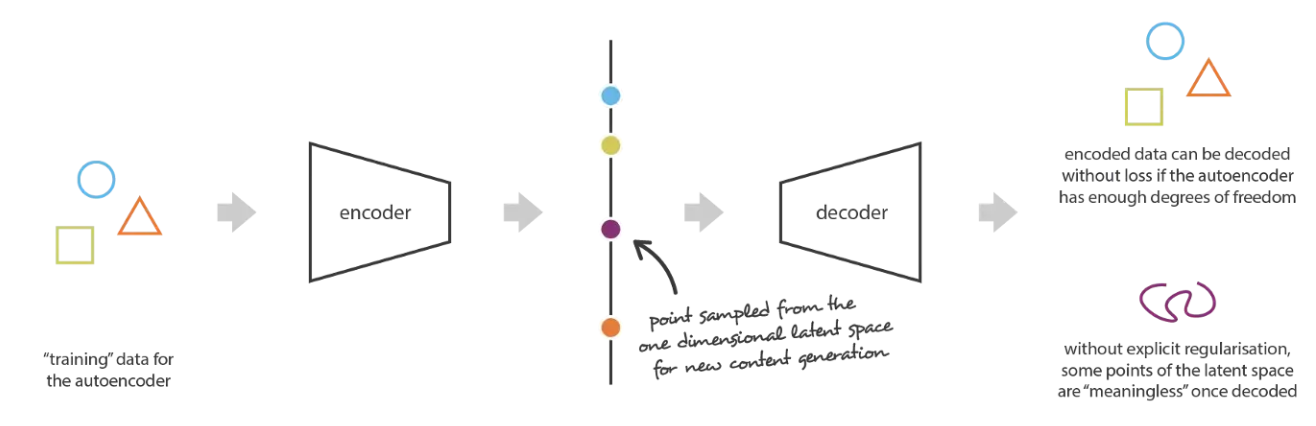
\includegraphics[width=1\textwidth]{images/AE_reg_problem.png}
    \caption{Не регуляризований простір кодування звичайного автоекодера має проблему при використанні в завданнях генерації нових об’єктів.}
\end{figure}
Розглянувши класичну структуру автоенкодера ми перейдемо до найбільш успішної його варіації - Варіаційного автоекодера, що показала прекрасні результати і є лідером у багатьох топ-чартах моделей побудови рекомендацій. Такий розвиток є наслідком Баєсового варіаційного підходу, що дає можливість навчатись не тільки на відомих реальних об’єктах а і на згенерованих самою моделею після вивчення і моделювання потрібного розподілу даних.

Також, однією із причині викоистання такого підходу є не регуляризованість простору прихованих змінних автоенкодера. На Рисунку 3.5 показана інтерпретація цієї проблеми.

Головна особливість варіаційного автоекодера є те, що він вчиться кодувати не вхідний сигнал мережі, а розподіл векторів прихованого простіру(коду).

Отже можна визначити наступні переваги автоенкодерів у завданнях рекомендацій:
\begin{itemize}
    \item Навідмінно від класичних моделей які можуть використовувати тільки один із джерел даних (оцінки взаємодії або текст) автоенкодери використовують широкий спектр гетерогенних даних таких як: оцінки, аудіо, зображення або відео.
    \item Автоенкодер через свою нелінійність краще вивчає вподобання користувачів, що призводить до більш високих оцінок метрик якості.
    \item Автоенкодер адаптивний до багатьох сценаріїв і більш ефективний у випадку боротьби із вхідним шумом у даних.
\end{itemize}
\subsection{Графові нейронні мережі}
Графові нейронні мережі - класс нейронних мереж які оперують даними у вигляді графів (Рис. 3.6). У більш широкому розумінні такий клас мереж можна віднести до геометричного глибинного навчання, в якому існуючі архітектури інтерпретують як графові нейронні мережі. Як приклад - у контексті комп’ютерного зору, зображення можна сприймати як граф пікселів, а у випадку обробки мови, графом представляють слова у тексті. 
До недавного часу більшість моделей векторизації графів були повільні і використовували  алгоритми на основі матричної факторизації або спектральної декомпозиції графів. Однак, додатково вони мали обмеження у використанні, при побудові графу, додаткової інформації, яка могла зберігатись у ребрах або вершинах. Поява графових нейронних мереж стала логічним подальшим розвитком досліджень у сфері побудови графових моделей і дозволило уніфікувати в один підхід минулі розробки.

\begin{figure}
    \centering
    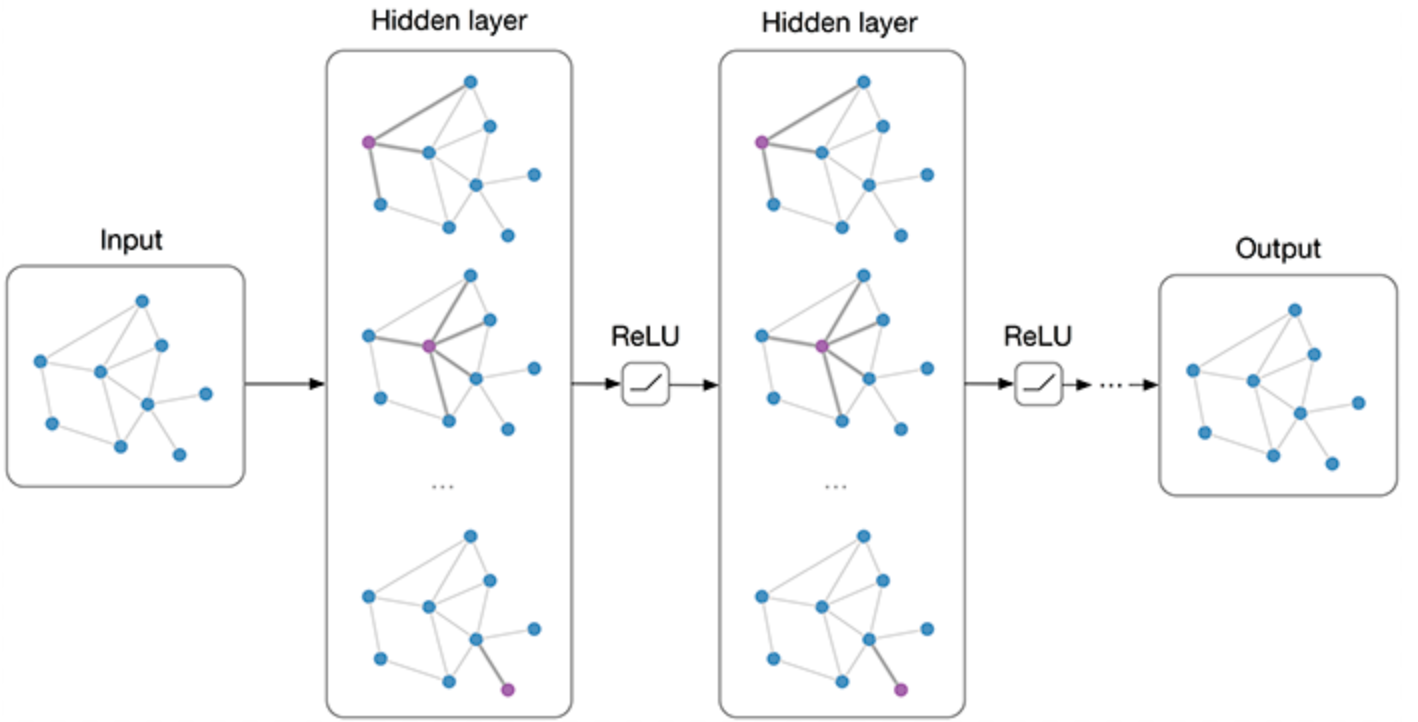
\includegraphics[width=0.8\textwidth]{images/GNN.png}
    \caption{GNN - тип нейронних мереж які напряму працюють із структурою графу.}
\end{figure}


В основі GNN лежить використання механізму передачі повідомлень (Message passing). Граф оброблюється набором модулів, які повязані між собою у відповідності до вузлів графу. Також, кожен із модулів пов’язаний із самими вузлами графа. Під час процесу навчання, модулі обновлюють свої стани і обмінюються інформаціюєю. 
Цей процес відбувається до моменту, поки модулі не перейдуть у стан рівноваги. Вихід GNN обчислюється на базі значень модулів кожного вузла графу.

Нехай, $\mathcal{G} = (\mathcal{V}, \mathcal{E})$ вхідний граф із набором признаків вершин $X \in \mathbb{R}^{d \times |\mathcal{V}|}$. І стоїть завдання побудувати латентне відображення $h_u$  для кожної $u \in\mathcal{V}$. На кожній ітерації GNN, відображення $h_u$ оновлюється агрегацією сигналів
із суміжних вершин  $\mathcal{N}_u$ (Рис. 3.7):
\[ h_u^{k + 1} = f_1^{k}(h_u^{k}, f_2^{k}({h_v^{k}, \forall v \in \mathcal{N}(u)}))\]
\begin{figure}
    \centering
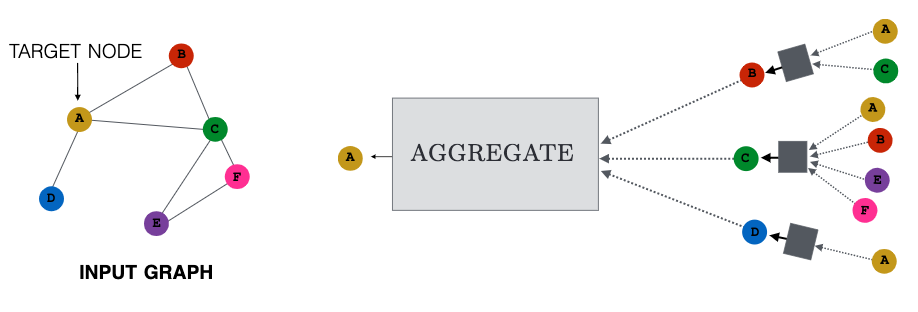
\includegraphics[width=0.8\textwidth]{images/Message_passing.png}
\caption{Ілюстрація агрегації сигналів сусідів для однієї вершини графу. Значення агрегації усереднюються.}
\end{figure}
де $f_1$ і $f_2$ відповідають за операцію оновлення і агрегації, які підбирають в залежності від ситуації. Повідомленням у графових нейронних мережах принято називати:
\[ m_{\mathcal{N}(u)} = f_2^{k}({h_v^{k}, \forall v \in \mathcal{N}(u)})\]

На кожній ітерації $k$, GNN $f_2$ - функція агрегації приймає на вхід набір прихованих значень сусідів, а функція $f_1$ оновлює ембединг об’єкту використовуючи повідомлення $m_{\mathcal{N}(u)}$ і значення із попередньої ітерації $h_k^{u}$.  Після  $K$ ітерацій message passing, ми отримуємо фінальні значення для кожної вершини на вихідному шарі:
\[z_u = h_u^{K}, \forall u \in \mathcal{V}\]
Під ітерацією $k$ можна розуміти глибину передачі повідомлень, чим він більший, тим більша відстань від $u$ до вершин які агрегуються. Такий підхід має ціль зібрати інформацію про структуру сусідніх елементів, а також про значення признаків їх вершин.

У разі використання моделі персептрону  Рів. 2.6 приймає наступний вигляд:
\[ h_u^{k} = \sigma \left(W_{self}^{k} h_u^{k-1} + W_{neigh}^{k} \sum_{v \in \mathcal{N}(u)} h_v^{k-1} + b^{k}\right)\]
де $W_{self}^{k}$ і $W_{neigh}^{k}$ матриці вагів мережі, а $\sigma$ не лінійна функція активації.

Графові нейронні мережі у задачах побудови рекомендацій знайшли своє використання у таких завданнях:

\begin{itemize}
    \item \textbf{Рекомендація послідовностей (Sequential Recommendation)}. Аналізуючи послідовнісь дій користувачів, такі моделі хочуть на основі деякого ланцюга подій  ${x_1, x_2, ..., x_n}$ довжини $n$ передбачити $x_{n+1}$ об’єкт (Рис 3.8).
    \item \textbf{Рекомедація на основі сесії}. Одна із найскладніших завдань. У моделі стоїть ціль передбачити $x_{n+1}$ об’єкт на основі активної сесії користувача, тобто в режимі реального часу.
    \item \textbf{Соціальні рекомендації}. Великі соціальні мережі використовують моделі для передбачування поведінки і побажань своїх користувачів. В майбутньому ці дані можуть бути використані для продажу або реклами (наприклад Facebook Ads).

\end{itemize}

\begin{figure}
    \centering
    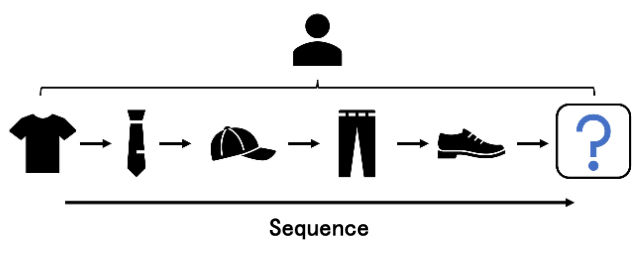
\includegraphics[width=0.8\textwidth]{images/Seq_rec.png}
    \caption{Ілюстрація завдання передбачення послідовності.}
    \end{figure}
\subsection*{Висновок}
У розділі розглянуто принцип роботи нейронної мережі прямого поширення на прикладі персептрону. Проаналізовано аріхтектури нейромереж на основі автоекодера і графової нейронної мережі. Розглянуто ключові деталі їх роботи: алгоритм навчання автоенкодера і механізм передачі повідомлень. Розглянуто принцип роботи і основні переваги використання вищезгаданих архітектур у завданнях побудови рекомендацій.
\section{МЕТРИКИ ОЦІНКИ ЯКОСТІ}

Система рекомендацій, як інструмент, повинна виконувати поставлені
їй задачі. Як приклад візьмемо задачі із області е-коммерції, а
саме ключові показники продуктивності бізнесу (Рис. 4.1):
\begin{itemize}
    \item CR(Conversion Rate)
    \item CTR
    \item LT(Life Time)
    \item LTV(LifeTime Value)
    \item Retention
    \item User Egagement
\end{itemize}
\begin{figure}[h]
    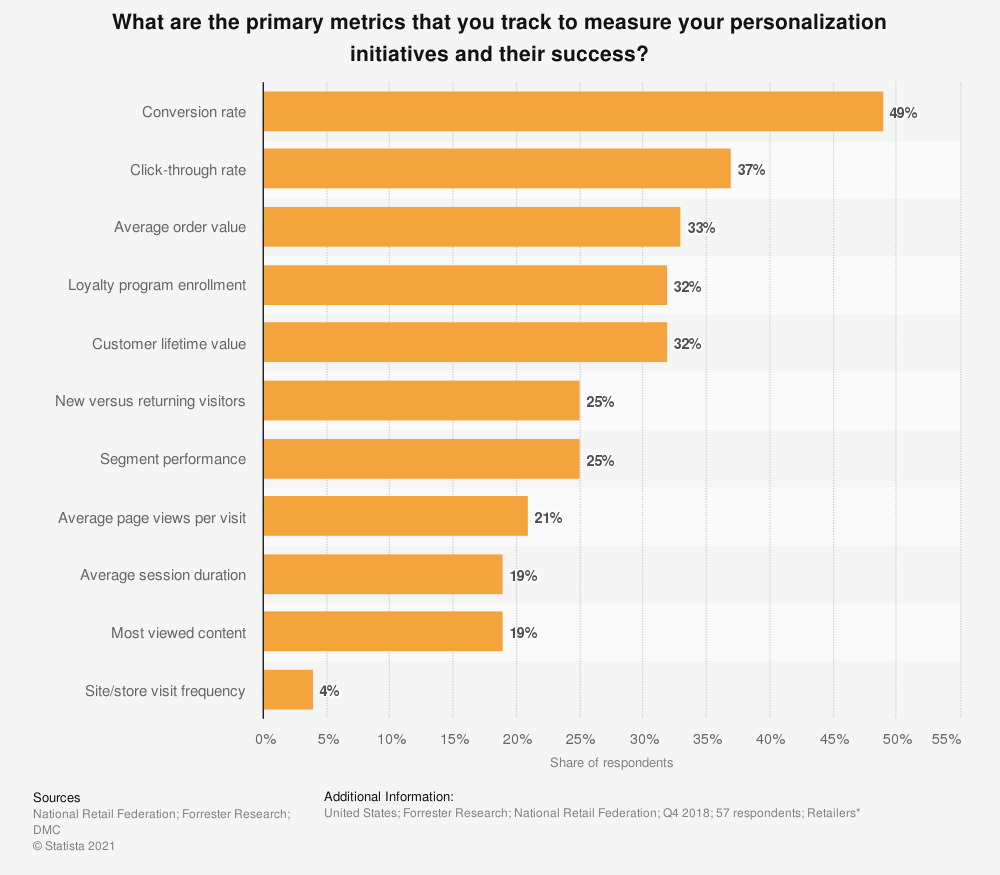
\includegraphics[width=1\textwidth]{images/E_commerce_metrics.png}
    \caption{Рейтинг популярності комерційних метрик}
    \label{fig:ecommerce_pop_metric}
\end{figure}

Найкращий спосіб визначити, чи покращує RS ці показники - провести A/B тест за допомогою відгуків користувачів.
Однак A/B тест, як правило, є дорогим і довготривалим у імплементації. Тому, перш ніж провести тест A/B, бажано
застосувати дешевший та швидший метод тестування в режимі офлайн,
щоб зменшити можливість значного падіння якості наданих рекомендацій.

Це призводить до розробки різних підходів, таких як тестування на
згенерованих даних та офлайн-оцінки, що є стандартним способом
порівняння продуктивності різних моделей. Важливо
підтримувати послідовність та рівномірність на всіх етапах,
включаючи метричний розрахунок.

\subsection{Класифікація метрик систем рекомендацій}
В силу специфіки нашої задачі, метрики системи можна умовно
поділити на групи взалежності від підходу -
\textbf{Метрики Класифікації},
\textbf{Метрики Ранжування},
\textbf{Метрики Новизни і різноманіття}. Введемо означення для опису метрик:
\begin{itemize}
    \item u  ідентифікатор користувача
    \item i  ідентифікатор об’єкта рекомендацій
    \item ${rec_k}$  список рекомендацій для користувача u із з top-k обєктів рекомендацій
    \item $rel(u)$  список релевантних обєктів для користувача u із тестового набору
    \item $rank(u,i)$  позиція i обєкту у списку рекомендацій $ rec_{k}(u)$
    \item $\mathbb{I}[\cdot] $  індикаторна функція
\end{itemize}
\subsection{Метрики класифікації}
Метрики класифікації оцінюють придатність до прийняття рішень систем рекомендацій. Вони є хорошим вибором для завдань визначення важливих або нерелевантних продуктів для користувача.

\begin{figure}
    \centering
    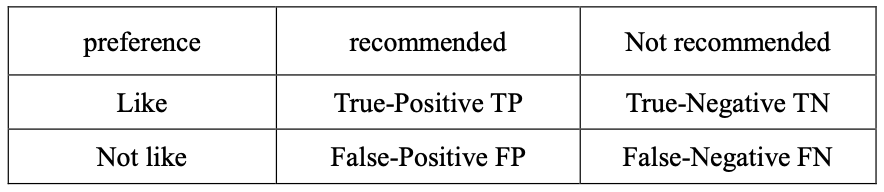
\includegraphics[width=0.7\textwidth]{images/confusion_m.png}
    \caption{Матриця помилок}
    \label{fig:conf_matrix}
\end{figure}
\subsubsection{Precision and Recall}
Метрики які широко використовуються у задачах класифікації знайшли своє використання і тут (Рис. 3.2):
\begin{align}
    Precision@k(u)=\frac{|rel(u) \cap rec_{}(u)|}{k} \\
    Precision = \frac{TP}{TP + FP}
\end{align}

\begin{align}
    Recall@k(u)=\frac{|rel(u) \cap rec_{k}(u)|}{|rel(u)|} \\
    Recall = \frac{TP}{TP+FN}
\end{align}
Precision можна інтерпретувати як частку об'єктів, що класифіковані як вірні та в той же час є вірними, і Recall показує, яка частка позитивного класу від всіх об'єктів вірного класу виявив алгоритм.
\subsubsection{F1-Score}
F1@K - це гармонічне середнє значення Precision@K і Recall@K, що допомагає спростити їх в одну метрику. Всі вищезазначені показники можна обчислити на основі матриці помилок(Рис. 3.2). Точна формула наведена нижче:
\[F1@k = 2 \times \frac{Precision@k \times Recall@k}{Precision@k + Recall@k} \]
Як ми бачимо, коефіцієнт F1 не враховує TN(True Negative). Це випадки, коли система рекомендацій не рекомендувала товар, який не має значення для користувача. Тобто метрика "сліпа" відносно певної групи обє’ктів рекомендацій. Цікавою та ідеально симетричною альтернативою є коефіцієнт кореляції Метьюса (MCC).
\subsubsection{Matthews correlation coefficient (MCC)}
Коефіцієнт кореляції Метьюса - це коефіцієнт кореляції між спостережуваною та прогнозованою бінарною класифікацією:
\[ MCC = \frac{TP\times TN - FP \times FN}{\sqrt{(TP + FP)\times(TP + FN)\times (TN+FP)\times (TN+FN)}}\]
Коли класифікатор ідеальний (FP = FN = 0) значення MCC становить 1, що вказує на ідеальну позитивну кореляцію.І навпаки, коли класифікатор завжди неправильно класифікує (TP = TN = 0), ми отримуємо значення -1, що представляє ідеальну негативну кореляцію.
\subsubsection{Hit Rate}
Приймає значення 1, коли хоч одна із рекомендацій є релевантною.
\[
    HitRate@k(u)=\mathbb{I}[|rel(u) \cap rec_{k}(u)| > 0]
\]
\subsubsection{Mean Average Precision}
Середня відносна точність(MAP) усереднюється для користувачів, і всі відмінності трапляються в розрахунку середньої точності.
\[
    AP@k(u)=\frac{1}{x}\sum\limits_{i \in rec_{k}(u)}\mathbb{I}[i \in rel(u)]Precision@rank(u,i)(u)
\]
\subsubsection{RocAuc}
Крива ROC (характеристика операційної кривої приймача) - це графік, що показує продуктивність моделі класифікації на всіх порогах класифікації (Рис. 4.3). Метрика використовує наступні складові:
\begin{itemize}
    \item TPR - True Positive Rate
          \[TPR = \frac{TP}{TP + FN}\]
    \item FPR - False Positive Rate
          \[FPR=\frac{FP}{TP + FN}\]
\end{itemize}
\begin{figure}
    \centering
    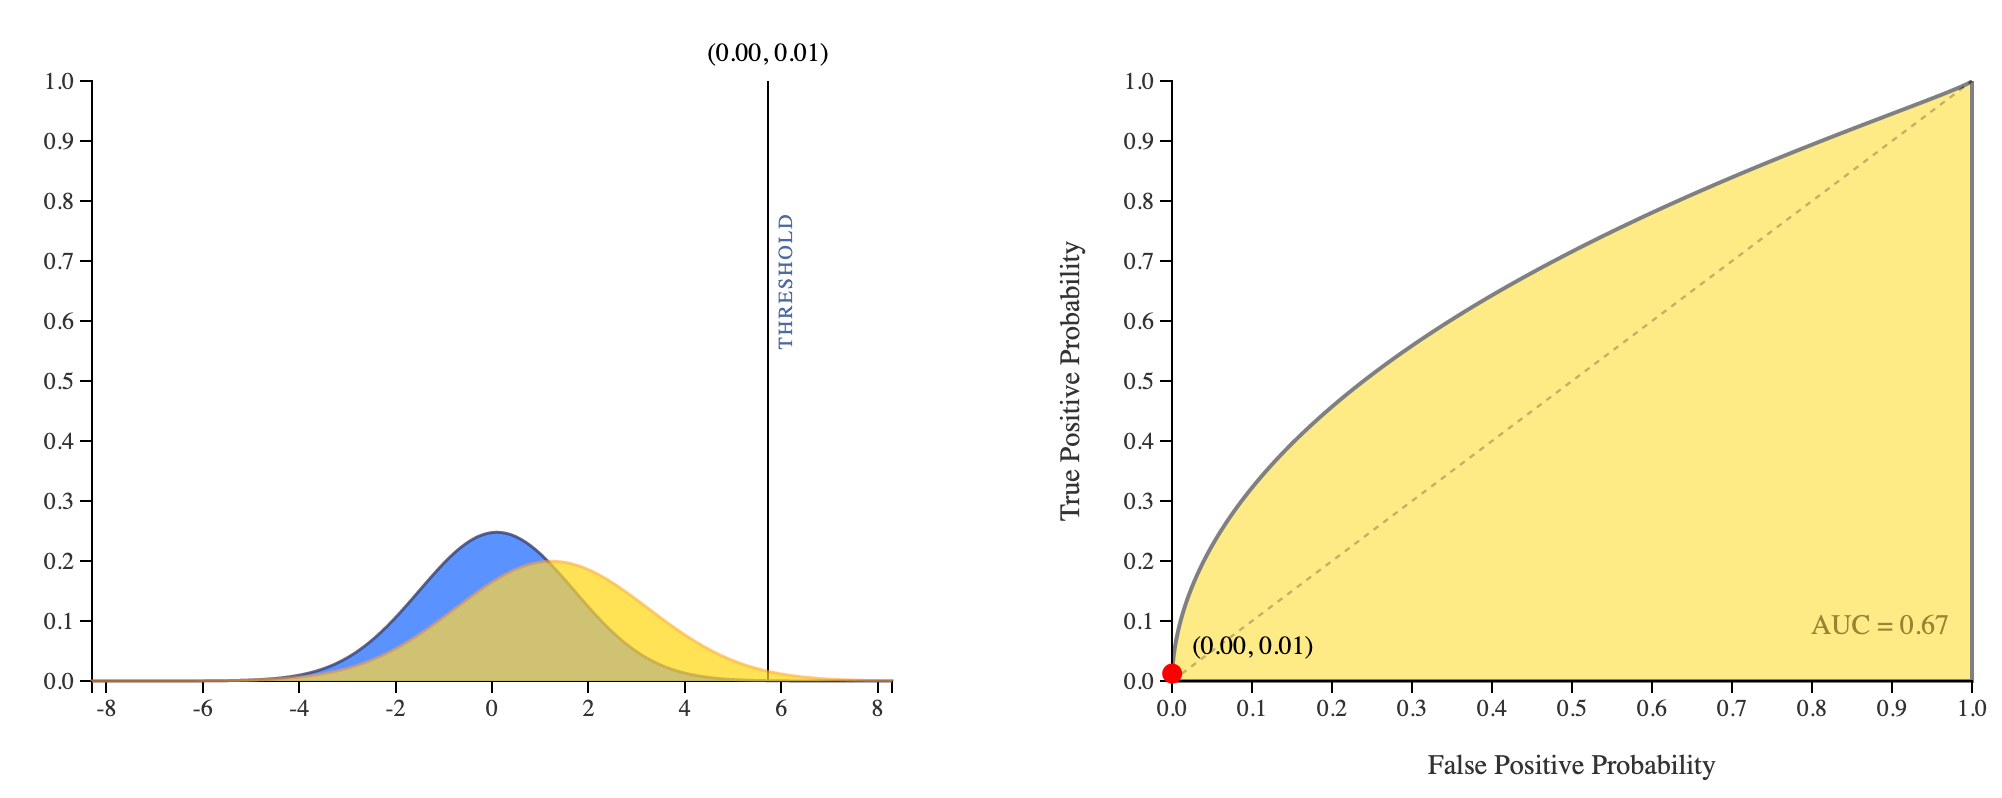
\includegraphics[width=0.8\textwidth]{images/auc_roc.png}
    \label{fig:auc_roc}
    \caption{Умовний приклад метрики ROC AUC}
\end{figure}
AUC походить від "Area under the ROC Curve". Тобто AUC вимірює всю  площу під кривою ROC від (0,0) до (1,1).AUC забезпечує сукупний показник продуктивності у всіх можливих порогах класифікації. Один із способів інтерпретації AUC - це як ймовірність того, що випадковий позитивний приклад буде оцінено більш високо, ніж випадковий негативний приклад.
AUC ціниться з наступних причин:
\begin{itemize}
    \item AUC інваріантний до масштабу. Він вимірює, наскільки добре оцінюються прогнози, а не їх абсолютні значення.
    \item AUC інваріантний до порогу чутливості. Він вимірює якість прогнозів моделі незалежно від того, який поріг класифікації обраний.
\end{itemize}

\subsection{Метрики ранжування}

\begin{figure}[h]
    \centering
    
\includegraphics[width=0.5\textwidth]{images/MLR-search-engine-example.png}
    \caption{Типова архітектура системи інформаційного пошуку}
\end{figure}

Метрики ранжування використовуются у системах рекомендації через
призму підходу як до задачі інформаційнного пошуку (Information
Retrival).

Інформаційний пошук (ІП) в обчислювальній та інформаційній науці -
це процес отримання ресурсів інформаційної системи, що
відповідають інформаційній потребі збору цих ресурсів. Пошуки
можуть базуватися на повнотекстовій або іншій індексації та на основі
вмісту. Отримання інформації - це наука пошуку інформації в
документі, пошук самих документів, а також пошук таких метаданих,
які описують дані, а також для баз даних текстів, зображень чи
звуків.

Автоматизовані системи пошуку інформації використовуються для
зменшення того, що називається перевантаженням
інформації. ІП-система - це програмна система, яка забезпечує
доступ до книг, журналів та інших документів; зберігає та керує
цими документами. Веб-пошукові системи - це найбільш помітні
ІП-програми.

\subsubsection{Cукупний інформаційний приріст}
 (Discounted Cumulative
Gain) - це показник рейтингу, який може прийняти довільні значення
релевантності.
У ІП він часто використовується для вимірювання
ефективності алгоритмів веб-пошукових систем або пов'язаних з ними
додатків. Використовуючи метрику оцінки релевантності
документів у наборі результатів пошуку, DCG вимірює корисність або
її приріст, на основі позиції елементів у списку
результатів. Чим вищий ранг обєкту у списку реезультатів тим
більше підсилюється його релевантність, а для нижчих зменшується.

Для використання метрики нам потрібно пряйняти наступні
припущення:
\begin{itemize}
    \item Існування деякої міри релевантності для елементів набору.
    \item Елементи із більш високою релевантністю приносять більше
          користі якщо вони знаходятся вище у списку (мають більш високі ранги)
\end{itemize}
% Формулювання метрики потрібно почати із $DCG$.Головна ідея - штрафувати елементи із великою релевантністю
% пропорційно до пониження їх рангу. 
Для штрафування використовуємо log reducing factor. Загальноприйнята формула для $DCG$:
\[
    DCG@k(u)=\sum_{i \in rec_{k}(u)}\frac{2ˆ{rating(u,i)} - 1}{log_{2}(rank(u,i) + 1)}
\]
$DCG$ обчислюється для одного набору документів (обєктів), для
можливості порівняння таких наборів вводять і використовують
$nDCG$, де $n$ відповідає за нормалізацію:
% \textit{ratings(u,i)} для зважування результатів. У RECSYS 
\[
    NDCG@k(u)=\frac{DCG@k(u)}{IDCG@k(u)}
\]
де $IDCG@k(u)$  (тобто $Ideal DCG$) максимально можливе значення
$DCG@k(u)$. Його ми можемо отримати у випадку ідеального
сортування набору обєктів рекомендацій довжини $k$. Для
цієї мети зазвичай використовуються рейтинги елементів із
тестового набору.
% Ми назвемо цю версію зваженою NDCG ($wNDCG$).

Також для бінарних обєктів розглядають наступну варіацію:
\[
    DCG@k(u)=\sum_{i \in rec_{k}(u)}\frac{\mathbb{I}[i \in rel(u)]}{log_{2}(rank(u,i)+1)}
\]

Можна передбачити наступні обмеження NDCG:
\begin{itemize}
    \item NDCG не штрафує за низьку релевантність самих обєктів.
          Якщо оцінки одинакові (наприклад [1, 1, 1] і  [1, 1, 1, 0])
          значення метрики буде одинакове. Потрібно використовувати
          нормування із відємним значенням для негативних елементів.
    \item Також метрика не є еффективною для малих k (набір
          рекомендації фіксованого розміру може швидко заповнюватись
          першими n елементами).
\end{itemize}
\subsubsection{Cередній взаємний ранг}
Mean Reciprocal Rank (MRR) або середній взаємній ранг - це середнє
значення зворотньої позиції (рангу) першого релевантного обєкту у
списку рекомендацій. Якщо жодних елементів не передбачано
правильно, він визначається як 0.
\[
    MRR@k(u)=\frac{1}{k}\sum_{i=1}^{|k|}\frac{1}{\min\limits_{i \in rel(u) \cap rec_{k}(u)}rank(u,i)}
\]
\subsubsection{Очікуваний взаємний ранг (Expected Reciprocal Rank)}
Припустимо, що система повертає користувачу рейтинговий список документів (рекомендацій), де ймовірність $p(q, d_{k})$, що документ задовільняє запит користувача:
\[ERR = \sum_{k=1}^{K}\frac{1}{k}p(q, d_{k}) \prod_{i=1}^{k-1}(1-p(q, d_{i}))  \]
Вибір обє’кта із певним рангом свідчить що користувач задоволений документом, ймовірність якого $p(q, d_{k})$. Також, це свідчить що всі рекомендації із вищим рейтингом  $1, ... ,k-1$ ймовірність яких $\prod_{i=1}^{k-1}(1 - p(q, d_{k}))$ не були обрані.

Для моделювання ймовірності що конкретна рекомендація буде обрана використовують так звану "редакційнку оцінку" (editorial grade) - цінність певного обєкту. В залежності від прикладної задачі можна ввести правила основані на схожості (із іншими типовими об’єктами), або передбачуванням моделі. В літературі розглядають 5 оцінок (0, 1, 2, 3, 4), де 0 це не релевантний об’єкт, а 4 дуже релевантний.
Тоді ймовірність за "редакційною оцінкою":
\[R(g):=\frac{2^{g}-1}{2^{g_{max}}}, g \in \{0, ..., g_{max}\}\]

\begin{figure}
    \centering
    \includegraphics*[width=0.3\textwidth]{images/edit_grade_prob_sample.png}
    \caption{Приклад розрахунку ймовірності для ERR}
\end{figure}

Тобто, переглядаючи результат пошуку на запит із оцінкою 3, є шанс 7/16, що користувач буде задоволений цим документом і, отже, припинить пошук, або із шансом 9/16 пошук продовжится (Рис. 4.5).

\begin{itemize}
    \item Однією приємною особливістю ERR є те, що вона завжди лежить між 0 до 1, причому 1 - найкраще. Це означає, що втрата внаслідок зіпсування будь-якого окремого прикладу обмежена.
    \item Метрика дає можливість зменшити вплив низького рангу на об’єкт. Важливість списку рекомендацій сильно падає при збільшенні його розміру (елемент із рангом 20 має множник 1/20 до своєї релевантності). ERR частково це нівелює.
\end{itemize}

\subsection{Метрики новизни і різноманітності}

Новизна та різноманітність є одним із важливих аспектів оцінки систем рекомендацій, і дозволяє більш широко підходити до оцінки кандидатів. Додатково, вказані властивості є надзвичайно корисними як із точки зору бізнесу, так і для самих користувачів. 

Прийняття кліків, переглядів або інших дій як докази прихильності користувача до контенту потребує великої долі впевненості, в тому що змодельовані оцінки справді віповідають потребам клієнта. Здебільшого, ми можем тільки надіятись що наші гіпотези будуть доказані.
Навчаючи моделі ми оперуємо лише тою частиної інформації, яку змогли зібрати.
Здебільшого, потреби користувачів є комплексні, динамічні, залежать від контексту (св’ято, пора року, час доби) і подеколи надзвичайно суперечливі.
Наприклад, перегляд мультфільму Ранго можна трактувати як прихильність до мультфільмів, або прихильність до комедій. Тому, передбачення вподобань є складним завданням, у якому не можливо досягнути ідеальної точності.

Одним із варіантів часткового вирішення таких проблем, є підхід у рекомендації надзвичайно різних по своїй природі об’єктів. Різноманіття кандидатів підвищує шанс того, що хоч одна із рекомендацій буде релевантною.
Враховуючи невизначеність щодо того, від яких характеристик залежить вподобання користувача, рекомендація фільму кожного жанру, як правило, окупається більше, ніж рекомендація, скажімо, трьох мультфільмів.

Різноманітність та новизна також знаходять мотивацію в бізнесі. Задоволеність клієнтів приносить користь бізнесу у вигляді посилення активності, доходів та лояльності клієнтів.
Крім цього, диверсифікація продукту - це відома стратегія зменшення ризику та розширення бізнесу. Більше того, це long tail sell - стратегія отримання прибутку від ринкових ніш, продаючи і отримуючи більш високу норму прибутку на дешевші продукти які важко знайти (Рис. 4.6).

Усі вищезазначені загальні міркування, звичайно, можуть бути замінені конкретними характеристиками конкретної області, ситуації та мети рекомендацій.
Наприклад, отримання списку подібних продуктів (наприклад, фотокамер) до одного, який ми зараз вибираємо, може допомогти нам уточнити наш вибір серед великого набору дуже подібних варіантів. Рекомендації можуть слугувати навігаційною допомогою в такого типу ситуації.
В інших областях є сенс споживати ті самі або дуже схожі предмети знову і знову, наприклад, покупки продуктів, одяг, тощо.

\begin{figure}
    \centering
    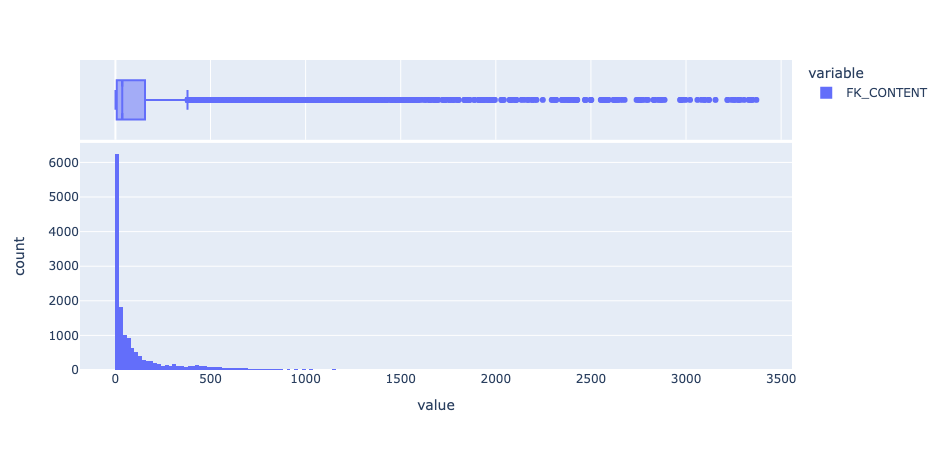
\includegraphics[width=0.8\textwidth]{images/long_tail.png}
    \caption{Типова гістрограма взаємодій користувачів, так званий "long tail" }
\end{figure}

Новизна та різноманітність суттєво різні, але пов'язані поняття (Рис. 4.7). Новизна, як правило, посилається на різницю між сучасним та минулим досвідом, тоді як різноманітність стосується внутрішніх відмінностей у елементах рекомендацій. Різноманітність, як правило, стосується набору предметів, і має відношення до того, наскільки різні предмети стосовно один одного. В основному, різноманітність оцінюється в наборі елементів, рекомендованих кожному користувачеві окремо, і, як правило, усереднюється у всіх користувачах загалом.

Загалом, варто розглянути такі наступні метрики систем рекомендацій.
\begin{figure}
    \centering
    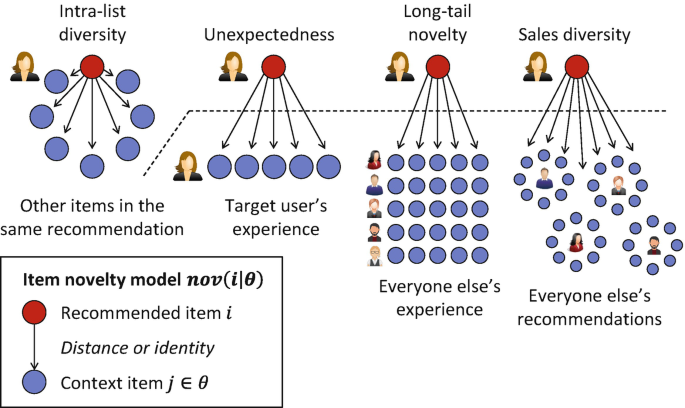
\includegraphics[width=0.7\textwidth]{images/novelity_diversity.png}
    \caption{Новизна і різноманітність у системах рекомендацій}
\end{figure}
\subsubsection{Зворотня середня частота (Mean Inverse Item Frequency)}
Використовуючи підхід ІП, частоту появи певного об’єкта у наборі взаємодій, можна інтерпретувати як міру популярності цього об’єкту. Ця частота подається у вигляді, знайомому нам із поняття інформаційної ентропії:
\[MIUF@k = -\frac{1}{|k|}\sum_{i \in k}log_{2}\frac{|U_i|}{|U|}\]
де $U_i$ множина користувачів які знайомів із об’єктом $i$. 
У перспективі така новизна на даних із довгим хвостом показує наскільки релевантний об’єкт відносно його популярності.

\subsubsection{Несподіваність (Unexpectedness)}

Несподіваність розглядають у контексті неочікуваного, але приємного досвіду.
Навідмінно від популярності, метрика цілком залежить від вподобань користувача і описує непохожість об’єктів рекомендацій із історичним досвідом користувача.

Існуює декілька варіацій Unexpectedness. Простіший варіант оцінює складність об’єктів у наборі. Під складністю розуміють наскільки не похожі об’єкти рекомендацій відносно елементів які користувач із великою ймовірністю вважає релевантними. Для створення порівняльної вибірки використовують тривіальні методи рекомендацій - вибір любимого актора, популярного реежисера, тощо.  
\[Unexpectedness@k = \frac{|K \backslash  PM|}{|K|}\]
У випадку коли у вибірці для порівняння присутні лише не відомі користувачу об’єкти: 
\[Serendipity@k = \frac{|(K \backslash  PM) \cap Rel|}{|K|}\]
де REL - це набір елементів які вважаються релевантними.
\subsubsection{Новизна (Temporal Novelity)}
Сприйняття користувача новизни також може розглядатися в межах взаємодії користувача з системою протягом деякого періоду. У цьому випадку ми визначаємо новизну як здатність систем рекомендацій не повторюватися, надаючи однакові або подібні рекомендації із часом. Ця перспектива оцінює здатність системи рекомендації генерувати нові знання про користувача та показує степінь адаптації рекомендацій до них.

\[ TN(R_u^{t}) = \frac {|R_u^{t} \bigcup_{\tau < t} R^{\tau}_u|} {|R^{t}_u|}\]
Де $R_u^{t}$ список рекомендацій у момент t.
\subsubsection{Різноманіття (Intra-List Diversity)}
Метрика оцінює наскільки відрізняються групи рекомендацій у користувачів. 
Ця оцінка є однією з найбільш вивчених у літературі, і стосується вирішення потреби користувачів у різноманітних рекомендаціях, уникаючи зайвих або монотематичних пропозицій. Метрика задається як середня парна дистанція між векторами об’єктів рекомендацій:
\[ ILD(R) = \frac{1}{|R|(|R| - 1)} \sum_{i,j \in R_u }ssim(i,j)\]  

Де у якості ssim може виступати одна із багатьох відомих метрик відстані між векторами.
\subsection*{Висновок}
На основі розглянутої літератури було відібрано і проаналізовано метрики систем рекомендацій. В результаті дослідження, метрики були поділені на 3 категорії в залежності від класу - метрики класифікації, метрики ранжування, метрики новизни і різноманіття. Для кожного класу наведено оцінки і їх опис.

\section{АНАЛІЗ АЛГОРИТМІВ РЕКОМЕНДАЦІЙ}
Моделі і алгоритми глибокого навчання на основі штучних нейронних мереж в останні роки знаходять своє використання у багатьох прикладних сферах інформатики. Цей підхід також показав прекрасні результати у порівнянні із класичними моделями у задачах побудови рекомендацій, що є наслідком уміння нейромереж знаходитити не лінійні і не тривіальні зв’язки у навчальних даних. А також, можливість використання в якості джерела даних як візуальну, так і текстову, контекстну інформацію.

\begin{figure}[H]
    \centering
    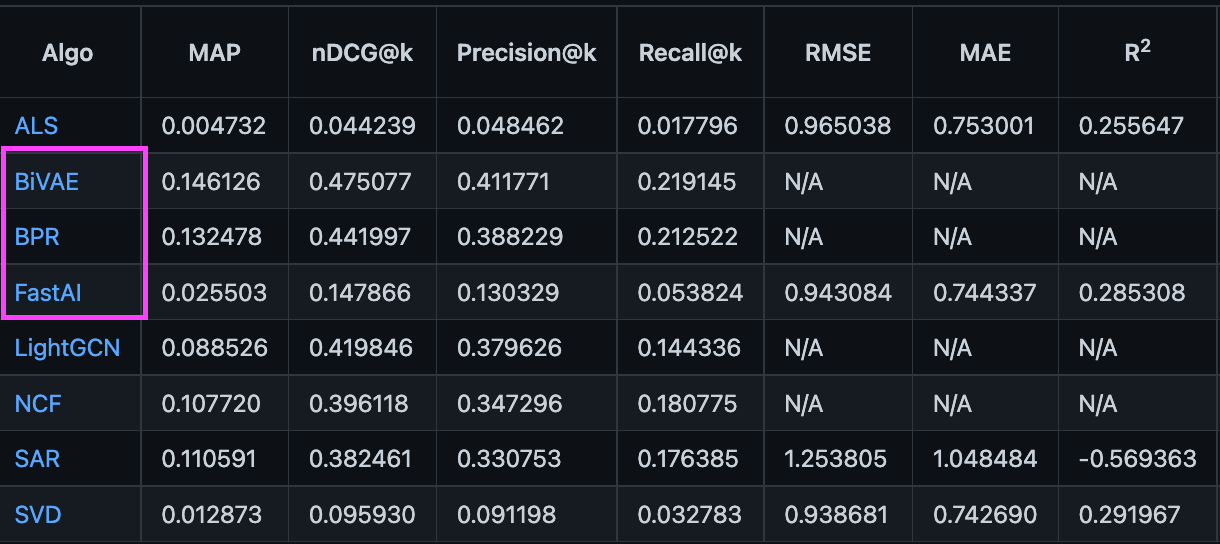
\includegraphics[width=0.8\textwidth]{images/NN_model_res.png}
    \caption{Порівняльні результати роботи моделей на основі нейромереж}
\end{figure}


Для практичних експериментів було обрано актуальні алгоритми рекомендацій які були представлені у останні декілька років. Із інших критеріїв було взято до уваги популярність у науковій сфері і використання у практичних реалізаціях.

Також, кожна розглянута модель відповідає певній групі алгоритмів для нейромережевої побудови рекомендацій.

\subsection{Алгоритм Neural Collaborative Filtering}

\begin{figure}
    \centering
    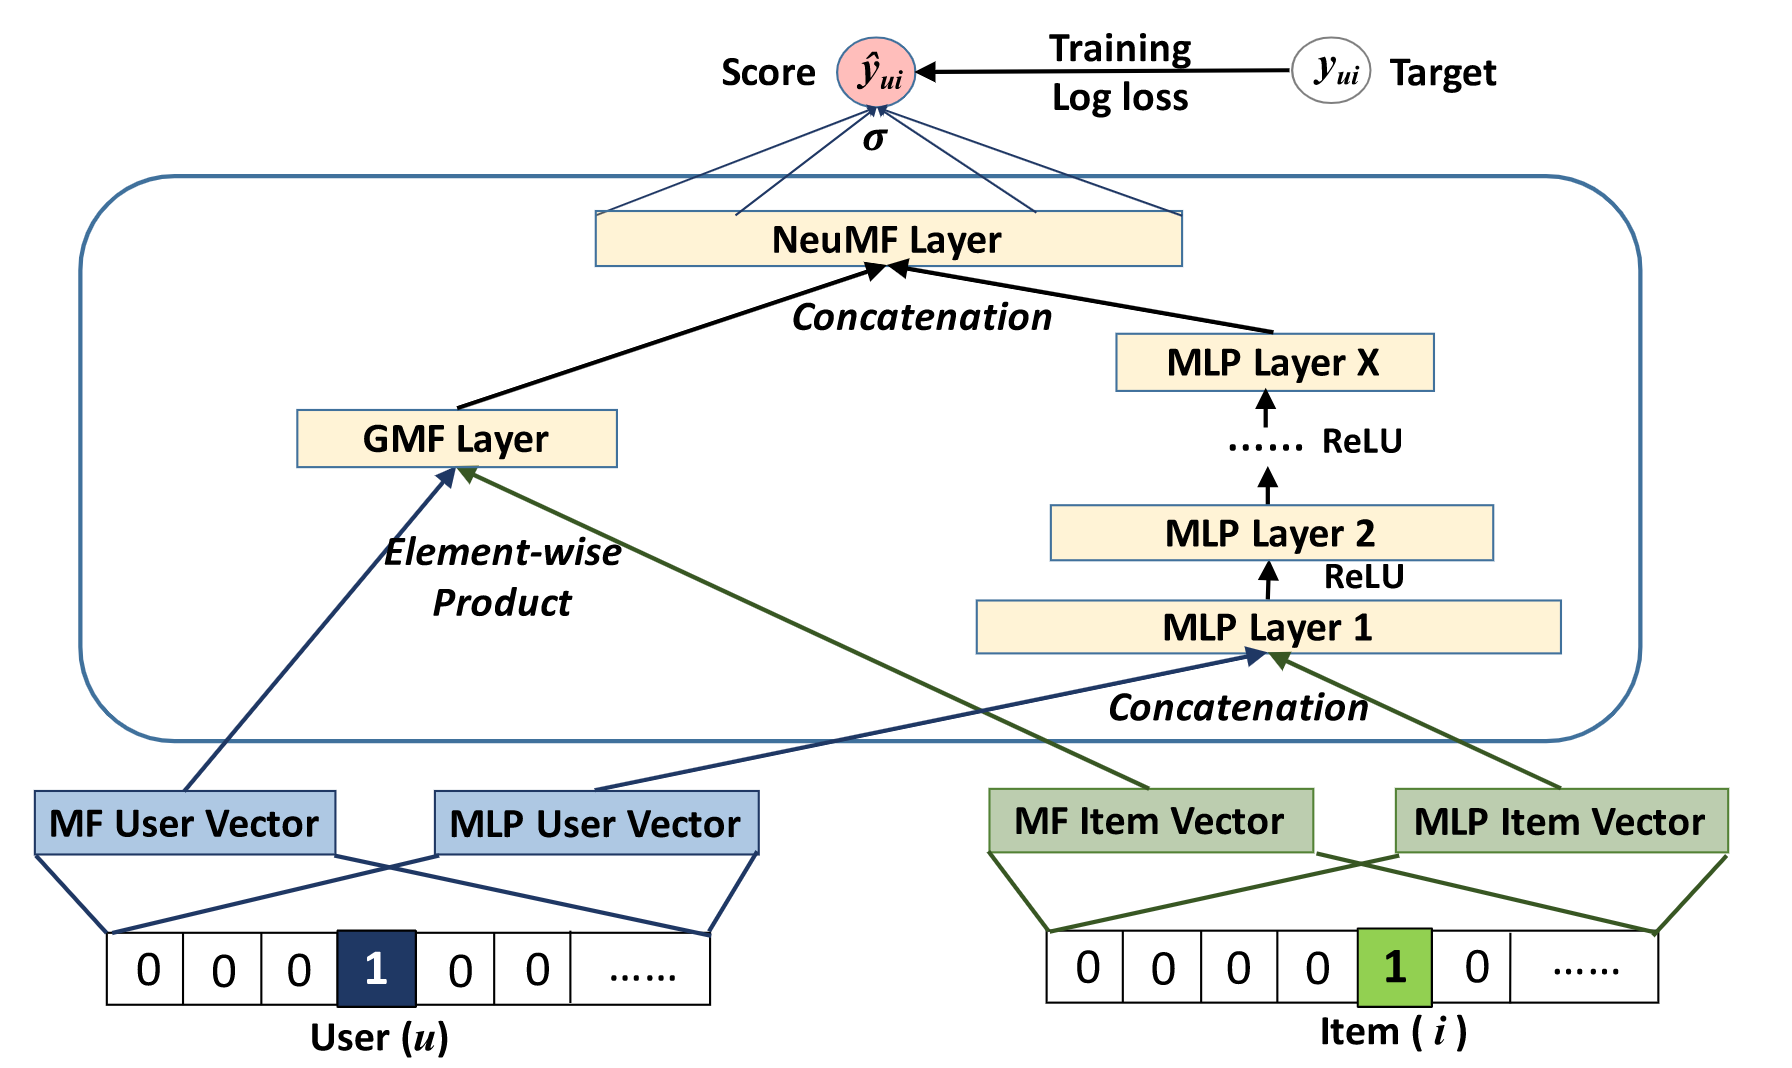
\includegraphics[width=0.8\textwidth]{images/NCF.png}
    \caption{Умовна будова NCF}
\end{figure}

Алгоритм нейронної факторизації NCF є потужним поєднанням алгоритму нейронної факторизації і багатошарового персептрону. Такий сплав лінійного і нелінійного підходу показує свою високу єфективність у моделюванні прихованих  взаємозв’язків між користвучем і об’єктом.

У звичайній матричній факторизації усі елементи знаходяться у одному прихованому просторі, що надає нам можливість визначити схожість між потрібними нам векторами використовуючи скалярний добуток/подібність косинуса або коефіціент Жаккара. Під матричною факторизацією маємо на увазі наступну модель оцінки взаємодії:
\[\hat{y}_{ui} = f(u,i|p_{u},q_{i}) = p^{T}_{u}q_{i} = \sum_{k = 1}^{K}p_{uk}q_{ik}\]

Але у задачах рекомендацій із неявною взаємодією (impicit feedback)
виникають проблеми із обрахуванням схожості внаслідок обмежень.

\begin{figure}
    \centering
    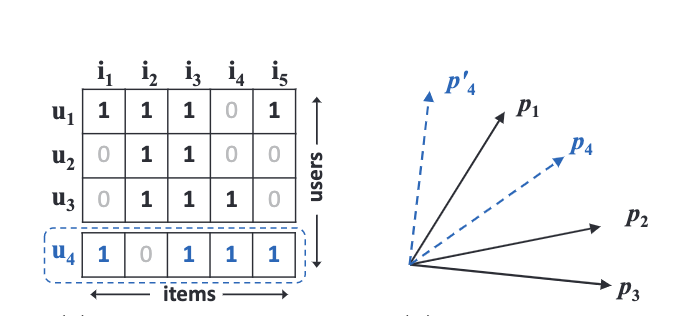
\includegraphics[width=0.8\textwidth]{images/MF_limitation.png}
    \caption{Зліва - матриця взаємодій користувача/об’єкта.Справа відображення у прихований простір. Положення вектора p4 відносно p3 ілюструє обмеженність. (Схожість p4 до p3 вища ніж до p2 але оптимально виразити ми не можемо).  }
\end{figure}

На вхід моделі подаються ембедінги користувача і об’єкта відповідно. Ці бінаризовані вектори можуть представляти широкий спектр корисної інформації - від вектора взаємодій до зжатих даних про вподобання користувача, історію або додаткову інформацію про об’єкт. Така особливість нівелює проблему холодного старту.

GMF(Generalized Matrix Factorization) - частина моделі яка відповідає за нейронну матричну факторизацію. Вхідні бінаризовані вектори можна інтерпритувати як приховані змінні користувача - $p_{u}$ і об’єкта відповідно $q_i$. Вхідний вектор що поступає на вхід:
\[\phi_{1}(p_{u}, q_{i}) = p_{u} \odot q_{i}\]
де $\odot$  відповідає за по елементний добуток. Вихідний вектор GMF:
\[\hat{y}_{ui} = a_{out}(h^{T}(p_{u} \odot q_{i}))\]
де $a_{out}$ відповідають за функцію активації і ваги вихідного шару.
При лінійній $a_{out}$ і юніт векторі $h$ відтворюється прямий вихід алгоритму матричної факторизації. Для базової імплеменатації була обрана сигмоїдна функція активації
\[ \sigma(x) = \frac{1}{1 + e^{-x}}\]
та логістична функція втрат.

MLP - використовуєтсья для моделювання не лінійної взаємодії. Це нейронна мережа прямого поширення із вежоподібною структурою (кожен наступний шар має вдвічі меншу розмірність). Формулювання мережі наступне:
\begin{align}
    \mathbf{z}_1 =\phi_1\left(\mathbf{p}_u, \mathbf{q}_i\right)=\left[\begin{array}{c}\mathbf{p}_u \\
                                                                              \mathbf{q}_i\end{array}\right],  \\
    \phi_2\left(\mathbf{z}_1\right) =a_2\left(\mathbf{W}_2^T \mathbf{z}_1+\mathbf{b}_2\right),         \\
    \cdots \cdots                                                                                      \\
    \phi_L\left(\mathbf{z}_{L-1}\right) =a_L\left(\mathbf{W}_L^T \mathbf{z}_{L-1}+\mathbf{b}_L\right), \\
    \hat{y}_{u i} =\sigma\left(\mathbf{h}^T \phi_L\left(\mathbf{z}_{L-1}\right)\right)
\end{align}

де $W_{x}$, $b_{x}$ і $a_{x}$ відповідають матриці вагів, вектору зміщення та функції втрат ReLU. Вибір функції активації обумовлений її властивістю до не насичення і більшою близькою до біологічної структури. Також, відомо що ReLu менш вразлива до перенавчання і є зручної при навчанні на розріджених даних.

Одними із важливих гіперпараметрів моделі є розмір вихідних векторів прихованих змінних. Чим вони більші, тим більш глибоко модель може генералізувати інформації про взаємодію. Тому для імплементації було відібрано декілька їх варіацій.

Фінальним поєднанням двох блоків моделі є шар NeuMF, на якому і обчислюється вихід мережі $\hat{y}_{u i}$. Комбінація результатів MLP і GMF відбувається за рахунок повнозвязного шару на вхід якого подається конкатенація двох векторів прихованих змінних. Використовуючи функцію активації ReLu ми отримуємо таку оцінку:
\begin{align}
    \hat{y}_{u i}=\sigma\left(\mathbf{h}^T\left[\begin{array}{l}
                                                        \phi^{G M F} \\
                                                        \phi^{M L P}
                                                    \end{array}\right]\right)
\end{align}

тут $\mathbf{h}$ це вектор вагів який задає вплив кожного блоку. Також, він може використовуватись для ініціалізації із препідготовлених вагів. Спочатку навчити із випадковомими вагами, а після досягнення збіжності використати ваги для фінального навчання:
\begin{align*}
    \mathbf{h} \leftarrow\left[\begin{array}{c}
                                       \alpha \mathbf{h}^{G M F} \\
                                       (1-\alpha) \mathbf{h}^{M L P}
                                   \end{array}\right]
\end{align*}
До моделювання функції втрат мережі потрібно підходити як до задачі бінарної класифікації (через бінаризацію вхідних даних і implicit формулювання). Тому функції втрат регресії не підходять (MSE  подібні). Значення прогнозувань моделі $y_{u i}=1$ інтерпритуємо, що обє’кт i важливий для u, а при 0, що ні.

Тому ми обмежуємо значення $y_{ui}$ інтервалі від [0, 1]. Додатково, це обмеження дозволяє використати ймовірносний підхід до інтерпритації.
Тоді функція правдоподібності приймає наступний вигляд:
\begin{align}
    p(\mathcal{Y}, \mathcal{Y}^{-} \mid \mathbf{P}, \mathbf{Q}, \Theta_f)=\prod_{(u, i) \in \mathcal{Y}} \hat{y}_{u i} \prod_{(u, j) \in \mathcal{Y}^{-}}(1-\hat{y}_{u j})
\end{align}
де $P \in \mathbb{R}^{M \times  K}$ і $Q \in \mathbb{R}^{N \times K}$ відповідає за матриці прихованих змінних, $\theta_{f}$ за параметри моделі функції взаємозв’язків f.
Наступну функцію потрібно мінімізувати використовуючи одим із бажаних варіантів градієнтного спуску:
\[
    L =-\sum_{(u, i) \in \mathcal{Y} \cup \mathcal{Y}^{-}} y_{u i} \log \hat{y}_{u i}+\left(1-y_{u i}\right) \log \left(1-\hat{y}_{u i}\right) .
\]
\subsection{Алгоритм VAE}

Для кожного користувача $u$ семплюється вектор $z_{u}$ розмірності K із багатовимірного нормального розподілу . K відповіє простору прихованих змінних і вміщує у собі інформацію про ключові структурні особливості об’єкта (у простому випадку для цифр це може бути їх колір, кут нахилу або ширина).
Для кожного вектора прихованих змінних нелінійна функція $f_{\theta}(.) \in \mathbb{R}^{I}$ надає оцінку щільності розподілу для набору  $I$ об’єктів рекомендацій $\pi(z_{u})$:
\begin{equation}
    z_u \sim \mathcal{N}(0, I_K), \pi(z_u) = softmax\{f_\theta(z_u)\}, x_u \sim Mult(N_u, \pi(z_u))
\end{equation}

У якості нелінійної функції виступає багатошаровий персептрон із параметрами $\theta$. Вихід цієї трансформації нормалізується функцією softmax і повертає
ймовірносний вектор $\pi(z_u)$ який містить значення для кожного об’єкту рекомендацій. Припускаємо що вектор $x_u$ належить поліноміальному розподілу із ймовірністю  $\pi(z_u)$. Функція правдоподібності для користувача $u$ відносно його прихованого відображення, нагороджує модель збільшуючи ймовірність ненульових елементів $x_u$:
\[ \log p_{\theta}(x_u|z_u) = \sum_i x_{ui} \log \pi_i(z_u)\]
Але через обмеженість $\pi(z_u)$, який сумується до одиниці, модель змушена підвищувати ймовірність на об’єктах які більш правдоподібно будуть обрані користувачем.
\begin{figure}
    \centering
    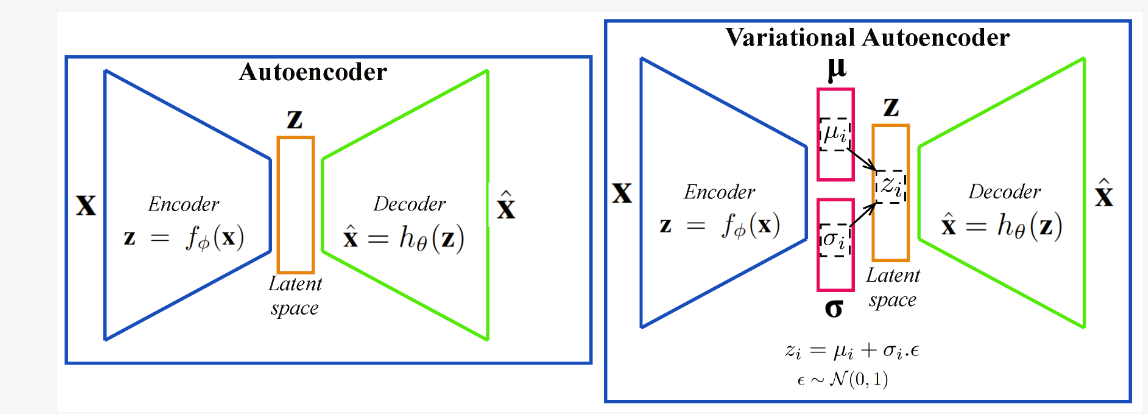
\includegraphics[width=1\textwidth]{images/AE.png}
    \caption{Ілюстративний приклад архітектури AE і VAE.}
\end{figure}
У задачі колаборативної фільтрації розглядають дві функції правдоподібності.
Допустим $f_{\theta}(z_u) \equiv [f_{u1}, \ldots, f_{uI}]^{T}$ є виходом генеративної функції $f_{\theta}(\cdot)$:
\begin{itemize}
    \item Функція правдоподібності Гауса:
          \[\log p_{\theta}(x_u|z_u) = - \sum_i \frac{c_{ui}}{2}(x_{ui} - f_{ui})^{2} \]
    \item Логістична функція:
          \[ \log p_{\theta}(x_u|z_u) = \sum_i x_{ui} \log \sigma(f_{ui} + (1 - x_{ui} \log(1 - \sigma(f_{ui}))))\]
\end{itemize}

Апроксимація $\log p_{\theta}(x_u|z_u)$, через його складність, виконується простішим нормальним розподілом $q(z_u) = \mathcal{N}(\mu_u, \sigma^{2}_u )$ із допомогою методів вараційного аналізу.

Для поняття відстані або відмінності між двома розподілами використовують відстань (дивергенцію) Кульбака-Лейблера. Яка є несиметричної мірою віддаленості один від одного двох ймовірностних розподілів, що задані на спільній множині елементарних подій. Відстань від розподілу $Q$ до $P$  позначається як $D_{KL}(P||Q)$, де $P$ сприймаємо за істинний розподіл, а $Q$ за розподіл який потрібно перевірити. У Теорії Інофрмації використовують інтерпретацію що $D_{KL}(P||Q)$ це кількість втраченої інформації при заміні істини $P$ на розподіл  $Q$:

\[ D_{KL}(P||Q) = \int_X p \log \frac {p}{q}\]

де $p = \frac{dP}{d\mu}$ і $q = \frac{dQ}{d\mu}$ неперервні функції із мірою $\mu$ на $X$.

Тому оптимізація варіаційних параметрів  $\{\mu_u, \sigma^{2}_u\}$ відбувається в наслідок  мінімізації  $ KL (q(z_u)) || p(z_u|x_u) $, яка є частиною функції втрат:
\[  \log p(x_u; \theta) \geq  \mathbb{E}_{q_{\phi}(z_u|x_u)} [ \log p_{\theta} (x_u|z_u)] -  KL (q_{\phi}(z_u|x_u) || p(z_u))  \equiv \mathcal{L}(x_u;\theta, \phi)\]

Цей вираз також відомий як розмір нев’язки або нижньої варіаційної границі (ELBO). Для її знаходження градієнтним спуском використовують так званий reparametrization trick який гарантує неперервність яка необхідна для back propagation. Ми семпюємо із деякого нормального розподілу  $\epsilon \sim \mathcal{N}(0, I_K)$ і модифікуємо $z_{u} = \mu_{\phi}(x_u) + \epsilon \odot \sigma_{\phi}(x_u)$. Що ізолює процесс генерації від пошуку градієнту напряму.
\subsection{Алгоритм Neural Graph Collaborative Filtering}
\begin{figure}
    \centering
    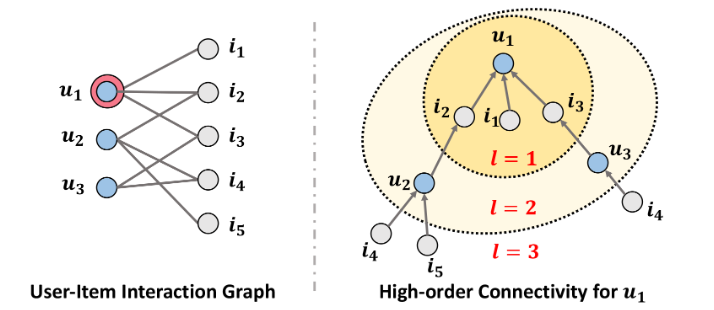
\includegraphics[width=0.8\textwidth]{images/interactions_graph.png}
    \caption{Приклад графу взаємодій користувач-об’єкт, а також ілюстрація взаємодій вищих порядків для NGCF }
\end{figure}
Алгоритм нейромережевої колаборативної фільрації на основі графів використовує підхід інтеграції взаємодій користувач-об’єкт у вигляді дводольного графу.
Такий підхід надає можливість моделювання взаємодій високого порядку, кодуючи у приховане відображення такі складні сигнали як поведінка користувача, що є надзвичайно ефективним у задачах рекомендацій для соціальних мереж.

На Рис 4.5 зображено ієрархію взаємодій для умовного користувача $u_1$. На першому рівні $l_1$ міститься інформація про об’єкти з якими $u_1$ контактував напряму (іншими словами, довжина шляху до яких дорівнює 1) і так далі для кожного наступного рівня (або шару). Використовуючи таку інтерпретацію ми описуємо подібність між користувачами на основі взаємодій. Наприклад ланцюг $u_1 \leftarrow i_2 \leftarrow u_2$ вказує на подібність поведінки $u_1$ і $u_2$ так як вони переглянули об’єкт $i_2$, а аналіз більш довшого шляху $u_1 \leftarrow i_2 \leftarrow u_2 \leftarrow i_4$ пропонує рекомендувати $i_4$ нашому цільовому користувачу $u_1$ ($i_4$ було обрано користувачем $u_2$,  і користувачем $u_3$ додатково).

Головна ідея алгоритму лежить у семплюванні прикладів взаємодій із навчального набору і ітеративного кодування інформації нейронною мережею виконуючи так званий information propagation. Що насичуює латентне відображення потрібною нам інформацією. Модель частково поворює структуру автоенкодера через присутність пари енкодер-декодер. На виході ми отримуємо оцінку релевантності об’єкта рекомендацій для користувача.   

\begin{figure}
    \centering
    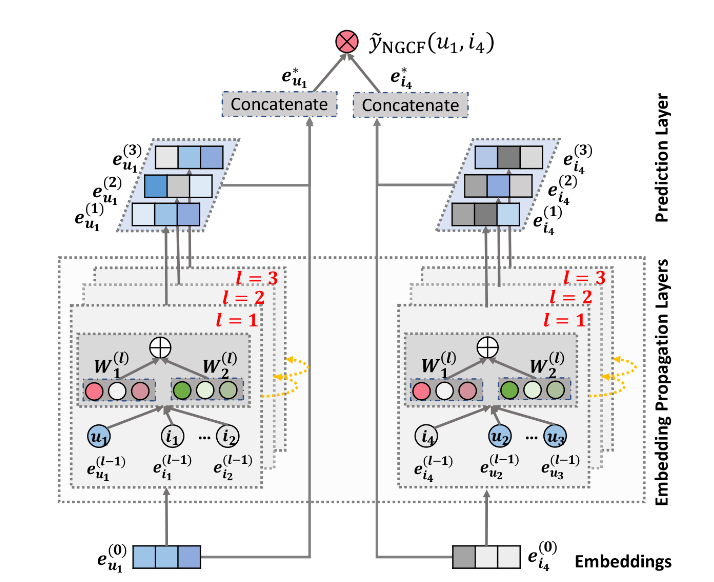
\includegraphics[width=0.8\textwidth]{images/NGCF.png}
    \caption{Архітектура моделі NGCF. Розглянуто приклад побудови оцінки рекомендації $i_4$ для користувача $u_1$}
\end{figure}

Модель складається із трьох компонентів - шару ініціалізації прихованих змінних, групи шарів насичення латентних змінних високорівневою інформацією, і шаром побудови оцінок (prediction). $e_u \in \mathcal{R}^{d}$ і $e_i \in \mathcal{R}^{d}$ вектор прихованих змінних користувача і об’єкта які описують їх поведінку, де $d$ відповідає розміру. Загальна матриця прихованих значень :
\[ E = [e_{u_1},\ldots, e_{u_N}] \times [e_{i_1},\ldots, e_{i_N}] \]. 

У подальшому, ми будемо навчати матрицю $E$ обновлюючи її значення. Цей процес називається агрегацією сигналів (message aggregation), і оперує так званим повідомленням:
\[m_{u \leftarrow i} = f(e_i, e_u, p_{ui})\]
де  $f(.)$ функція кодування повідомлення, що використовує в якості входу наші ембедінги $e_i$ і  $e_u$, $p_{ui}$ відповідає за коефіціент віддаленості для взаємодій і штрафує пропорційно відстані між $u$ до $i$.
Розглядаємо наступну функцію кодування:
\[ m_{u \leftarrow i} = \frac{1}{\sqrt{|N_{u}| |{N_{i}|}}} (W_1e_i + W_2(e_i \odot e_u))\]

Де $W_1$, $W_2$ є матриці вагів нейромережі які відбирають корисну інформацію для передачі. А $\frac{1}{\sqrt{|N_{u}| |{N_{i}|}}}$ відповідає за 
фактор віддаленості.

Зібравши інформацію із кожного сусіда $u$ ми обновлюємо $e_u$ використовуючи функцію активації LeakyReLU (дозволяє малий сигнал у випадку неактивації нейрону): 

\[  e_u = LeakyReLU(m_{u \leftarrow u} + \sum_{i \in \mathcal{N}_u} m_{u \leftarrow i})\]

де LeakyReLU:
\[ LeakyReLU(x) = \begin{cases}
    x, \text{if $x > 0$} \\
    0.01 x
\end{cases}\]
$m_{u \leftarrow u} = W_1 e_u$ відповідає за збереження сигналу із попередніх ітерацій.
\subsection*{Висновки}
Було проаналізовано моделі побудови рекомендацій на основі нейромереж. 
Обрано для експерементального дослідження моделі нейромережевої факторизації, варіаційного автоенкодера і графової колаборативної фільтрації. Для розглянутих алгоритмів було досліджено принцип їх функціонування, архітектуру, функції активацій, моделювання функцій втрат,  наведено інструкції для реалізації.
\section{АНАЛІЗ ФАКТОРІВ ВПЛИВУ}
Внаслідок розробки великої кількості нових рекомендаційних алгоритмів постало критичне питання у вітсутності єдиного підходу до оцінки їх еффективності, що призводитть до нерепродуктивних та несправедливих результів їх порівняння.

Також, побудова кожної системи рекомендацій складається із багатьох етапів які можна класифікувати на дві умові групи:
\begin{itemize}
    \item Фактори залежні від моделі
    \item Фактори не залежні від моделі
\end{itemize}
Кожен із них критично впливає на результат і залежить один від одного. Більше того їх оптимальні значення і характеристики не відомі. Тому важливо їх детально дослідити.

Фактори не залежні від моделі відповідають специфічним рішенням при пректуванні системи без прямого впливу на сам алгоритм і методів його оптимізації (тобто говоримо про вибір та підготовку навчальної вибірки, деталей проведення валідації).

Інші фактори, навпроти, включають у себе вибір таких речей як функція втрат, оптимізатор і метод регуляризації.
Розглядаючи типовий процес побудови рекомендацій варто виділити наступні  етапи:
\begin{enumerate}
    \item Вибір спліт методу (Dataset Spliting Method).
    \item Вибір метрики якості (Evaluation Metric Selection).
    \item Формулювання функції втрат для оптимізації (Loss function design).
    \item Методологія негативного семплінгу (Negative Samoling Strategy).
    \item Стратегія ініціалізації вагів (Parameter Initializer Selection).
    \item Вибір алгоритму оптимізації (Model Optimizer Selection).
    \item Вибір методу регуляризації (Regularization Term /  Dropout).
    \item Критерії останова (Early Stop Mechanism).
    \item Донавчання вагів (Hyper Params Tuning).
\end{enumerate}
Для кожного із вищевказаних факторів впливу відберемо кандидатів для експерементального дослідження. Нашою метою є пошук оптимального підходу до побудови ефективної моделі рекомендацій.
\begin{figure}
    \centering
    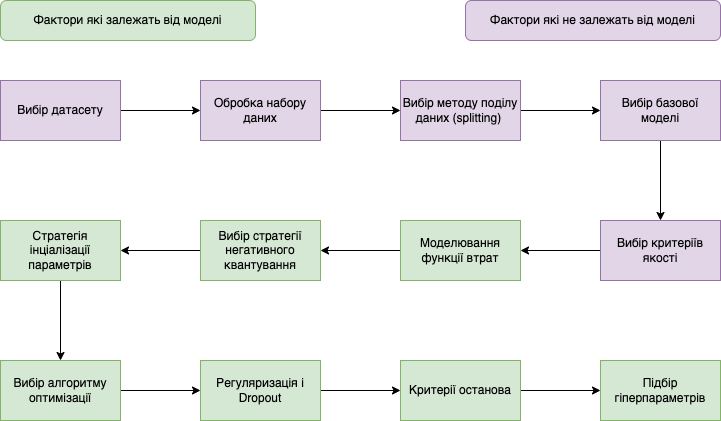
\includegraphics[width=0.9\textwidth]{images/FactorsTypes.png}
    \caption{Розглянутий пайплайн із поділом факторів впливу на категорії}
\end{figure}
\subsection{Вибір спліт методу}
Розглянувши набори даних які використовують для побудови рекомендацій, потрібно звернути увагу на розділ датасету на навчальну вибірку і вибірки для тестування (валідації). Валідація виконується для упередження перенавчання моделі, тобто алгоритм перестає широко генералізовуватись і починає змінювати ваги виключно під навчальні екземпляри. Після падіння метрик якості протягом 3-10 епох потрібно зупинити навчання і перейти до тестування на фільній вибірці.

Вибір спліт методу залежить від структури даних, а саме від присутності у них відмітки про час виконання дії. Що, надає можливість обрати одну із двох стратегій поділу.

У класичному підході в задачах машинного навчання, ми вважаємо що кожен зразок навчальної вибірки є не залежним один від одного. І не розглядаємо ймовірність коваріацій між взаємодіями одного користувача у розрізі часу (час взаємодій не впливає на використання). У цьому випадку використовують так званий поділ за співвідношенням. Тобто, ми ділимо датасет на групи відносно деякої пропорції, зазвичай $80\%$ на $20\%$, $80\%$ відходить на навчальну вибірку (разом із валідацією), а $20\%$ на тестування.

Другий можливий підхід - це поділ відносно часу. У навчальній вибірці беруть k спостережень певного користувача із максимальним timestamp (відміткою часу) t, а у тестовий набір попадають наступні n екземплярів із  timestamp більше t.
Тобто ми перевіряємо здатність моделі передбачити n наступних взаємодій.
\subsection{Підготовка даних}

\textbf{Для тестового набору}. Для завдання побудови рекомендацій потрібно зберігати повноту вибірки для тестування відносно користувачів. Що значить, що для кожного користувача який попадає у даний набір потрібно зберігати одинакову кількість його спостережень (наприклад не менше 5 оцінок на 1 унікальний user\_id).
У таблиці 7.1 наведено розраховані розміри вибірок для кожного користувача.
\begin{table}[]
    \centering
    \caption{Середня кількість екземплярів для кожного унікального користувача}
    \begin{tabular}{|c|c|c|c|}
        \hline
        Тип        & ML-1M & LastFm & Netflix \\ \hline
        Навчальний & 86    & 39     & 161     \\ \hline
        Тест       & 64    & 10     & 84      \\ \hline
    \end{tabular}
    \label{tab:size_of_split}
\end{table}

\textbf{Для тренувального набору}. Дані проходять додаткову фільтрацію від неактивних користувачів. Усі користувачі кількість взаємодій яких менше порогового значення видаляються із навчальної вибірки. Розглядаємо такі порогові значення [без фільтрації, 5, 10] 


\subsection{Вибір метрики оцінки якості}
Із великого різноманіття розглянутих метрик, було обрано шість основних метрик: Precision@k, Recall@k, MAP, HitRatio,  Mean Reciprocal Rank, NDCG. 
Для метрик які оцінюють фактичну присутність релевантних обєктів у рекомендаціях (*.@k) розглядаємо k у інтеравалі між [10,50].
\begin{figure}[H]
    \centering
    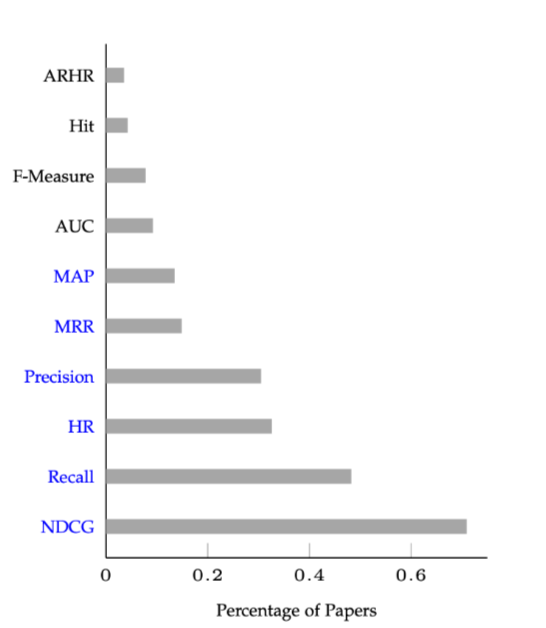
\includegraphics[width=0.6\textwidth]{images/metric_hist_papers.png}
    \caption{Розподіл використання метрик у наукових статтях}
\end{figure}

Метрики оцінюють передбачування моделей із точки зору класифікації і ранжування. Додатково потребує оцінка значень метрик різноманітності. Формулювання яких наведено у Розділі 4. 

\subsection{Стратегії негативного семплювання}
Вибірка об’єктів рекомендацій часто досягає надзвичайно великих розмірів.
Так, як моделі на виході повертають оцінку релевантності для цих об’єктів, на 
кожній ітерації навчання потрібно обновлювати ваги і розраховувати передбачення для кожного елементу. Що є не ефективно із точки зору вартості обчислень. Додатково, більшість користувачів знайомі лише із малою вибіркою елементів. Тому відсутність оцінки/взаємодії може вказувати не на низьку релевантність, а на те що об’єкт їм не відомий.

Для вирішення цієї проблеми використовують негативний семплінг. 

Його ідея полягає у відборі певної групи елементів, які не оцінені користувачем в минулому. 

В літературі розглядають декілька варіантів семплювання: із нормального розподілу, семплювання на основі низької популярності і семплювання із елементів високої популярності.

\begin{itemize}
    \item \textbf{Семплювання із нормального розподілу}. Обираємо n об’єктів керуючись їх ймовірністю.
    \item \textbf{High popularity sampling}.На основі розрахованих оцінок популярності обираємо top n кандидатів. Відсутність оцінки у невідомого,але популярного об’єкта явно вказує на низьку релевантність для користувача, порівняно із випадковим кандидатом.
    \item \textbf{Low popularity sampling}. Співпадає із high popularity, але вибираємо елементи із хвоста.
    \item Комбінування обох підходів.
\end{itemize}

\subsection{Стратегії ініціалізації параметрів}

Зазвичай у моделях побудови рекомендацій присутній набір параметрів, оптимізація яких навчає алгоритм. Їх вид залежить від обраної архітектури моделі і може бути як матрицею взаємодій, так і вагами нейромереж.
Привильний підхід до їх ініціалізації приводить до скорішого навчання і сходимості. Для моделей які будують приховане відображення взаємодій (латентні фактори) типовим є використання рівномірного $\mathcal{U}(0, a)$ і нормального $\mathcal{N}(0, \sigma^{2})$ розподілів, із значеннями $a = 1$ і $\sigma = 0.01$ відповідно.

Нейромережі особливо чутливі до початкових значень вагів. При не оптимальному підході, функція втрат змінюватись не буде, навіть після декількох десятків епох. Занадто малі значення приводять до затухання, коли функції активацій у нейронах залишаються неактивними (навіть у випадку використання таких функцій як LeakyReLU). Великі значення, навпроти, приведуть до зривних градієнтів.

У завданнях побудови рекомендацій із допомогою нейронних мереж використовують метод ініціалізації Ксавєра:
\[ W_{ij} \sim \mathcal{U}(- \frac{1}{\sqrt{n_{in} + n_{out}}}, \frac{1}{\sqrt{n_{in} + n_{out}}}) \]

Де $W_{ij}$  матриці вагів нейромереж, $n_{in}$, $n_{out}$ розмір вхідного і вихідного шару.

\subsection{Вибір методу оптимізації моделей}

\begin{figure}
    \centering
    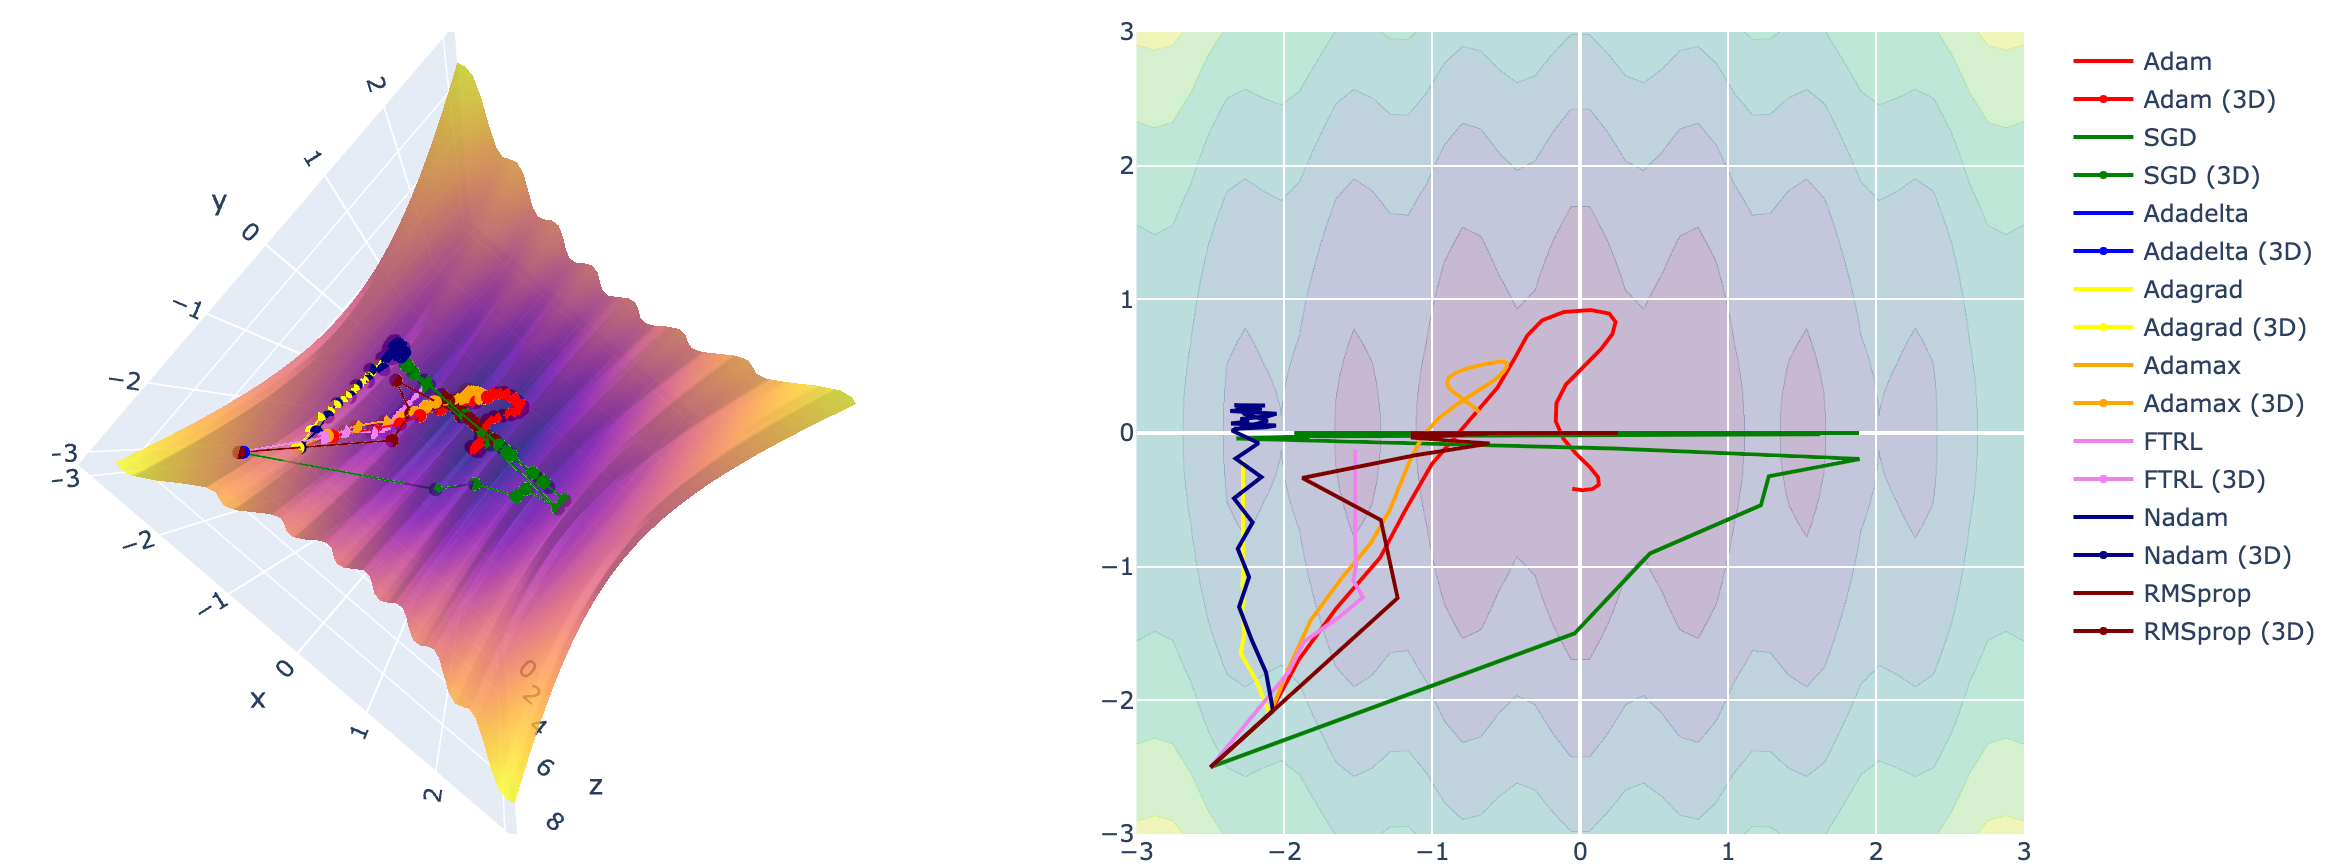
\includegraphics[width=0.9\textwidth]{images/sgd.png}
    \caption{Результат роботи різних варіантів градієнтного спуску}
\end{figure}

Оптимізатор використовується для оновлення параметрів моделі, мінімізуючи функцію втрат у пошуках глобального мінімуму. Різні оптимізатори впливають на роботу алгоритмів рекомендацій.

\textbf{Градієнтний спуск}.
Один із найпопулярніших ітераційних методів оптимізації першого порядку, основа багатьох наступних його варіацій. Розглядається задача пошуку локального мінімуму деякої функції $\mathcal{L}: \mathbb{R}^{n} \rightarrow \mathbb{R}$:
\[\mathcal{L} \rightarrow \min_{\theta \in \mathbb{R}^{n}}  \]
Ідея методу полягає в тому, щоб виконати оптимізацію в напрямку найшвидшого спуску, який задається антиградієнтом  $-\nabla_{\theta} f$:
\[\theta_{t+1} = \theta_{t} - \lambda  \nabla_{\theta} \mathcal{L}(\theta_t) \]
де $\lambda$ обирається одним із декількох варіантів:
\begin{itemize}
    \item Константа, у цьому випадку метод може не зійтись.
    \item Дробовим кроком, який змінюється.
    \item Найшвидшим cпуском : $\lambda_t = \arg \min_{\lambda} \mathcal{L} (\theta_t) - \lambda \nabla_{\theta} \mathcal{L}(\theta_t) $.
\end{itemize} 
Критерій останова для градієнтного спуску:
\[|\mathcal{L}(\theta_{t+1}) -  \mathcal{L}(\theta_t)| < \epsilon\]
де $\epsilon$ наперед задане невідємне число.

\textbf{Стохастичний градієнтний спуск}.Коли алгоритм проходить через навчальний набір, він виконує вищезазначене оновлення для кожного елемента датасету. Виконуючи перетасування, можна виконувати декілька проходів до збіжності, вибираючи оптимальний крок $\lambda$.

\[\theta_{t+1} = \theta_{t} - \lambda  \nabla_{\theta} \mathcal{L}(\theta_t, (u,i)) \]

\textbf{Пакетний градієнтний спуск}. Результат подальшого розвитку градієнтного спуску. В результаті експериментів було виявлено ефективність обновлення вагів сумою групи (пакету) елементів. Тобто, на одній ітерації значення вагів акумулюються і оновлюється їх сумою. Що прискорює збігання

\[\theta_{t+1} = \theta_{t} - \lambda  \nabla_{\theta} \mathcal{L}(\theta_t, B(u,i)) \]

\textbf{Адаптивний градієнт AdaGrad}. У завданнях обробки мови, фільтрації спаму чи побудови рекомендацій вхідний сигнал, тобто дані, часто бувають розріджені (У наших датасетах, наприклад Sparsity 99.99+\%). Така ситуація приводить до того що інформативні признаки зустрічатимуться достатньо рідко, і із іншої сторони, глобальні шаблони будуть зустрічатись надзвичайно часто (більшість користувачів знайомі із фільмами Володар Перстнів). Тому, було б зручно, визначати наскільки деякий признак часто зустрічається у навчальній вибірці, або як часто він приводить до активації нейронів. Ідея вирішення достатньо проста - ми будемо зберігати для кожного параметру мережі частоту його обновлення. І у випадку коли параметр навчається повільно (частота обновлень низька) ми будемо збільшувати його вплив.  
\[ \theta_{t + 1} = \theta_t - \frac{\lambda}{\sqrt{G_t + \eta}} \cdot \nabla_{\theta}\mathcal{L}(\theta_t)\]
де $G_t$ відповідає за частоту оновлення, а $\eta$ є деякий ненульовий фактор щоб вберегти ділення на 0. У параметра який часто обновлюється, великий $G_t$, і його вплив штрафується. Додатково, метод не сильно чутливий до вибору $\lambda$, достатньо обрати його один раз.
\newpage
\textbf{RMSProp}. Адаптивний градієнт має властивість затухати при великих значеннях $G_t$. Модифікацію, що вирішує проблему паралічу алгоритму називають RMSProp. 
\[ \theta_{t + 1} = \theta_t - \frac{\lambda}{\sqrt{\mathbb{E}[g^{2}_t] + \eta}} \cdot \nabla_{\theta}\mathcal{L}(\theta_t)
\]
Ми все ще збираємось оновлювати ваги, які занадто часто оновлюються, але замість повної кількості оновлень ми будемо використовувати квадрат  середнього градієнту в історії. Ми використовуємо експоненціальне згасаюче середнє $\mathbb{E}[g^2]$:
\[\mathbb{E}(g^{2})_t = \gamma \mathbb{E}[g^{2}]_{t-1}+ (1 - \gamma)g^{2}_t\]
% \subsection{Регуляризація}
\subsection{Критерії останова та Регуляризація}
\begin{figure}
    \centering
    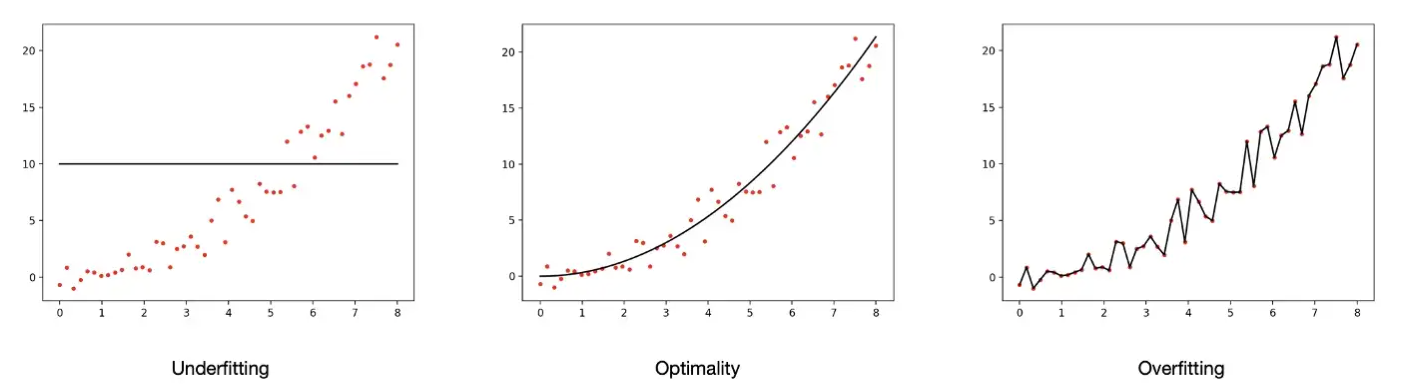
\includegraphics[width=1\textwidth]{images/fiting_problems.png}
    \caption{Приклад недонавчання, перенавчання і оптимального стану функцій втрат}
\end{figure}
У машинному навчанні використовуються різні стратегії для боротьби з проблемою перенавчання, яка приводить до гіршої генералізації, тим самим досягаючи низької ефективності на тестувальній вибірці (Рис. 6.4). Власне, найбільш широко використовувані методи регуляризації включають регуляризацію, механізм dropout та раньої зупинки.

\textbf{Регуляризація}. Як правило, фактор інтегрується в функцію втрат, щоб допомогти уникнути перенавчання під час навчання моделі рекомендації. В основному використовують два види, а саме регуляризація L1 та L2 (які також відомі як норми). Норма L1 відома як Манхетенська відстань, яка є найбільш природним способом вимірювання відстані між векторами. Це сума величин векторів у просторі, де всі компоненти вектора зважуються однаково. Норма L2 є найпопулярнішою нормою, також відомою як евклідова норма, відповідає  найкоротшій відстані між двома точками. 
Головними відмінностями у використані цих двох норм: L1 регуляризація намагається оцінити медіану даних, коли L2 оцінює середнє.
Додатково L1 норма виконує функцію feature selection -  відбирає лише важливі признаки, що корисно, враховуючи велику кількість признаків у завданнях Глибокого навчання.

\begin{figure}
    \centering
    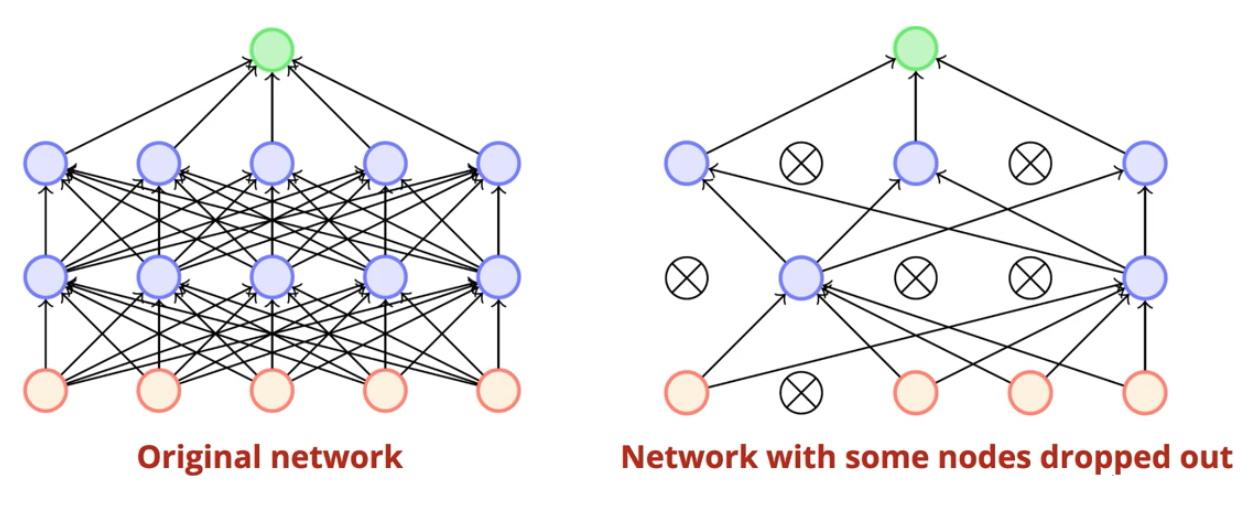
\includegraphics[width=1\textwidth]{images/dropout.png}
    \caption{У результаті Dropout, кожен нейрон із деякою ймовірністю може бути ”виключеним”}
\end{figure}
\textbf{Dropout}. Широко прийнятий у Глибокому навчанні метод, для упередження перенавчання. Ключова ідея полягає в тому, щоб випадковим чином відключити нейрони (разом із їх зв’язками) із мережі під час тренувань, що заважає мереді занадто сильно адаптуватись (Рис 6.5) . Отже, вводиться додатковий гіперпараметр, тобто ймовірність збереження нейрона Р, для контролю інтенсивності виключення. Типові значення P для нейронів прихованих шарів  знаходяться в діапазоні від 0,5 до 0,8.

\textbf{Механізм ранньої зупинки}. Рання зупинка - це також форма регулізації, яка використовується для уникнення надмірного перенавчання. Основна проблема моделей побудови рекомендацій(наприклад, LFMS та DLM) полягає у виборі кількості навчальних епох. Занадто багато епох можуть призвести до надмірної підстановки вагів до навчального набору даних, тоді як занадто мало може призвести до слабкої моделі. Рання зупинка - це метод, який дозволяє нам вказати довільну велику кількість навчальних епох і припинити навчання, як тільки  продуктивність моделі перестає вдосконалюватись на валідаційному наборі протягом декількох епох.
\subsection{Підбір гіперпараметрів}
Кожен гіперпараметр заданий набором можливих значень (тобто простором пошуку) на основі емпіричного знання, а оптимальне налаштування отримується шляхом проходженням через увесь простор пошуку. Такий підхід називається Grid Search. Основним його недоліком є обчислювальна нефективність, а у випадку великої кількості гіперпараметрів, його використання не доцільне. Припустимо, модель має m гіперпараметрів, де кожен параметр має у середньому n можливих значень, модель потрібно навчати NM разів, щоб знайти оптимальні значення для всіх гіперпараметрів.

RandomSearch, використовує одинакой піхід, тільки простір можливих значень вибирається випадково. 

Одним із більш оптимальних підходів, є так званий Bayesian HyperOpt.
Підхід байєсівської оптимізації фокусується на моделі ймовірності $P(score| configuration)$, яка оновлюється через ітеративний процес завдання якого є максимізація оцінки, враховуючи конфігурацію "C”. Hyperopt приймає байєсівську оптимізацію як свою передумову, зробивши деякі варіації в процесі вибірки, визначення та звуження простору пошуку та алгоритмів для максимізації моделі ймовірності.
\subsection*{Висновки}

У розділі розглянуто широкий набір фаторів впливу на якість моделей побудови рекомендацій. Представлено їх поділ відносно характеру впливу. Проаналізовано природу факторів, запропоновані варіації факторів для експериментального дослідження.
% \newpage
% \section{ДЕТАЛІ ВПРОВАДЖЕННЯ}
% У розділі наведено інформацію про деталі реалізації експериментів, ціллю яких є знаходження оптимальних параметрів розглянутих алгоритмів рекомендацій на основі результатів метрик якості. А також порівняння впливу не залежних від моделі факторів.

% \subsection{Датасети}
% \begin{figure}[H]
%     \centering
%     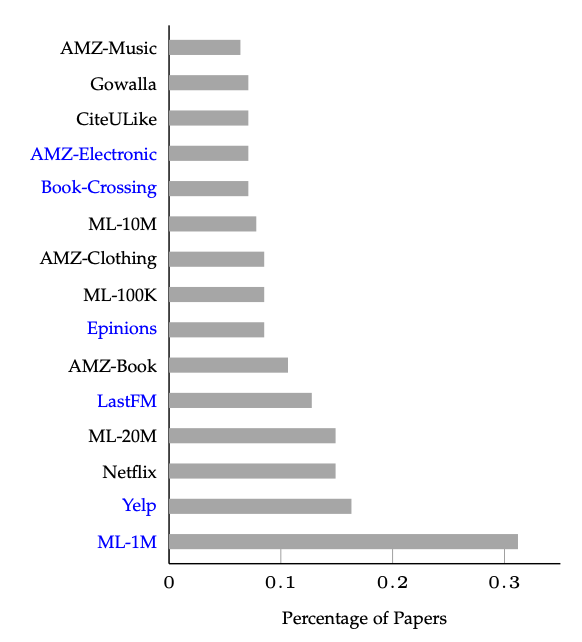
\includegraphics[width=0.6\textwidth]{images/dataset_dist.png}
%     \caption{Розподіл використання наборів даних у наукових статтях.}
% \end{figure}
% Для практичних еспериментів, а також навчання і валідації моделей будо обрано відкриті набори даних які є загально прийняті і використовуються для порівняння у академічній сфері (Рис. 18). Для кожного датасету проведений розвідувальний аналіз даних (EDA) для оприділення їх основних структурних особливостей і відмінностей. Кожен набір є зрізом БД приватних комерційних компаній, тому можна вважати що поведінка моделей відповідає реальним результатам.

% \subsubsection{Movielens 1M \cite{MovilensDataset}}
% Набір даних Movielens (ML-1M) є найпопулярнішим серед великого різноманіття датасетів. Movielens -  це мережева система рекомендацій фільмів для користувачів на базі їх відгуків і оцінок. Існує із 1996 року і містить у собі більше 11 мільйонів оцінок для 8600 об’єктів.
% \begin{figure}[H]
%     \centering
%     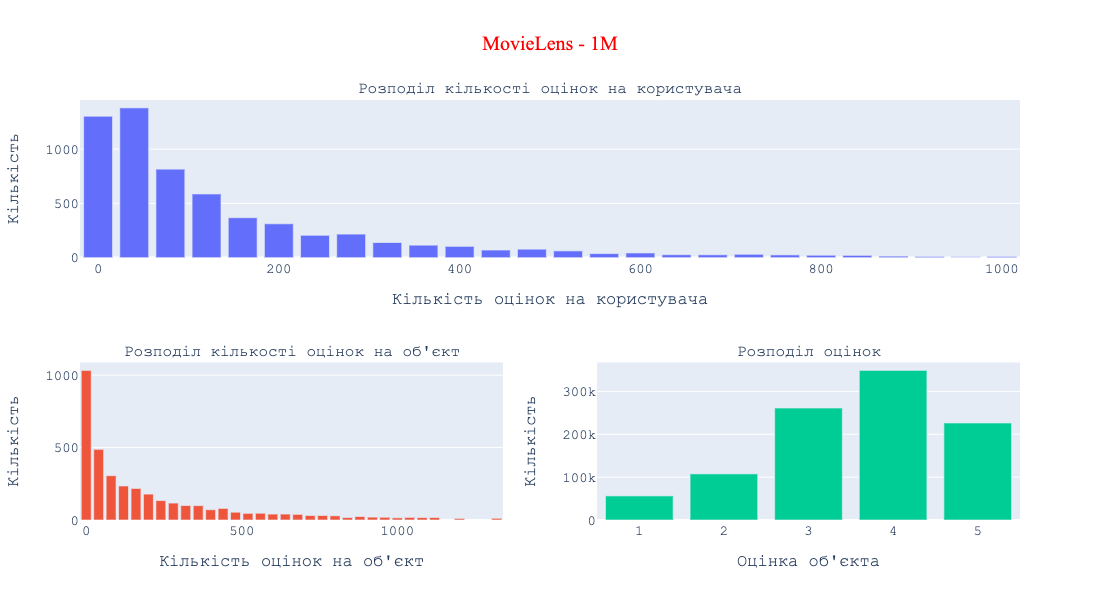
\includegraphics[width = 1\textwidth]{images/ML-1m_stat.png}    
%     \caption{EDA для набору даних Movielens (ML-1M) }
% \end{figure}
% Структура набору наступна: 
% \begin{itemize}
%     \item $item\_id$ індентифікатор користувача.
%     \item $user\_id$ індентифікатор об’єкта рекомендацій.
%     \item $score$ оцінка.
%     \item $timestamp$ дата і час дії.
% \end{itemize}

% Для аналізу відібрано 3706 об’єктів рекомендацій (фільмів) із 1 000 036  оцінок від корисутувачів. Що надає не менше 20 відгуків на один об’єкт.
% \begin{table}[H]
%     \centering
%     \caption{Характеристика набору даних Movielens 1M}
%     \begin{tabular}{|c|c|}
%         \hline
%         Загальна статистика      & Значення \\ \hline
%         Кількість взаємодій      & 1 000 029                    \\
%         Кількість користувачів   & 6 040                        \\
%         Кількість об’єктів       & 3 706                        \\
%         Розрідженність           & 99.9553\%                    \\
%         Середня оцінка           & 3.58 / 5                     \\ \hline
%         Взаємодій на користувача &                              \\ \hline
%         Середнє                  & 165.6                        \\
%         Медіана                  & 96.0                         \\ \hline
%         Взаємодій на об’єкт      &                              \\ \hline
%         Середнє                  & 269.89                       \\
%         Медіана                  & 123.5                        \\ \hline
%     \end{tabular}
%     \label{tab:ML-1m}
% \end{table}
% Більшість оцінок приймають значення від 3 до 4-5. У розподілі взаємодій чітко замітний лівий перекіс, що типово для даних такого роду. Розрідженість висока.


% \subsubsection{LastFm \cite{LastFMDataset}}
% Набір даних LastFm містить у собі інформацію про музику яка прослуховується у медіа плеєрах користувачів. Структурно датасет подібний до ML-1M, але додатково присутня інформація про ключові теги класу для об’єктів. Теги можуть описувати жанр, автора, додаткову ключову інформацію, що є зручним і може бути використано для насичення моделей.


% \begin{figure}[H]
%     \centering
%     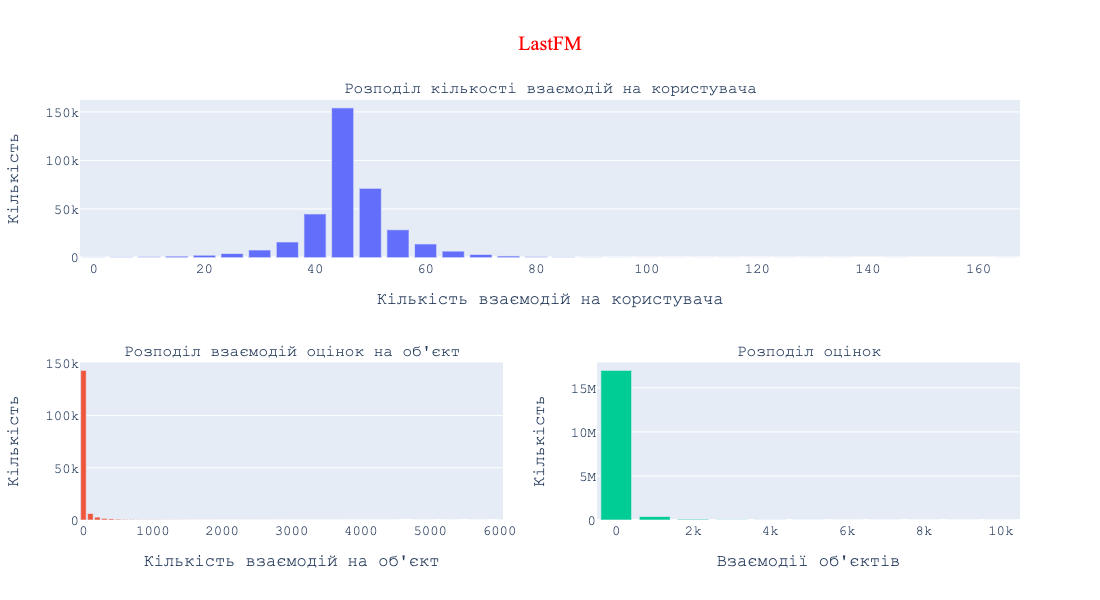
\includegraphics[width = 1\textwidth]{images/LastFM_stat.png}    
%     \caption{EDA для набору даних Last.fm}
% \end{figure}

% \begin{table}[H]
%     \centering
%     \caption{Характеристика набору даних LastFM}
%     \begin{tabular}{|c|c|}
%         \hline
%         Загальна статистика      & Значення \\ \hline
%         Кількість взаємодій      & 17 535 654                    \\
%         Кількість користувачів   & 358 868                        \\
%         Кількість об’єктів       & 160 113                        \\
%         Розрідженність           & 99.9996\%                    \\\hline
%         Взаємодій на користувача &                              \\ \hline
%         Середнє                  & 48.23                        \\
%         Медіана                  & 48.0                         \\ \hline
%         Взаємодій на об’єкт      &                              \\ \hline
%         Середнє                  & 108.10                       \\
%         Медіана                  & 6.0                        \\ \hline
%     \end{tabular}

%     \label{tab:LastFM}
% \end{table}

% \subsubsection{Netflix \cite{NetflixDataset}}
% Набір даних Netflix є одним із найбільших відкритих датасетів із реальними даними. Набір був створений під егідою проведення змагання Netflix Prize. Ціллю якого було розробка системи рекомендацій, переможець який добився найвищих показників якості отримав призову винагороду у розмірі 1 мільйон доларів. Датасет має класичну структуру: включає у собі дані про оцінки користувачів фільмів які були переглянути користувачами. Для кожного екземпляру є відмітка про час оцінки. 

% Дані мають типовий розподіл, і явно замітний перекіс. Із цікавого, через великий розмір і характер домену (рекомендація фільмів), датасет є одним із найнасичених. Розподіл оцінок - стандартний ([3, 4, 5]). Більше 90\% користувачів оцінили менше ста об’єктів.
% \begin{figure}[H]
%     \centering
%     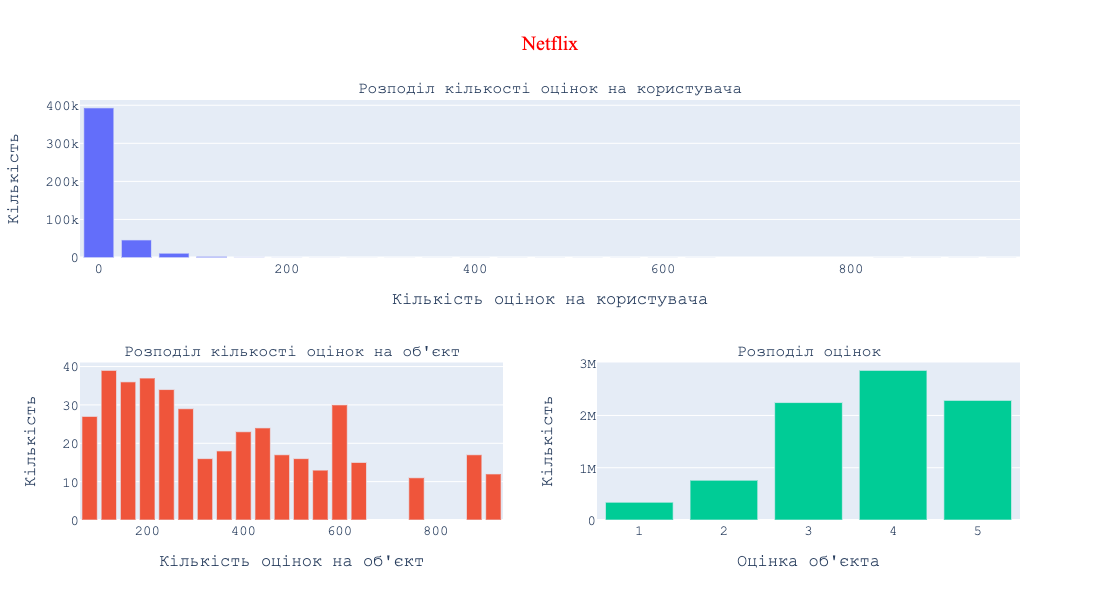
\includegraphics[width = 1\textwidth]{images/netflix_stat.png}    
%     \caption{EDA для набору даних Netflix}
% \end{figure}
% У Таблиці 7.3 наведено докладна характеристика набору.
% \begin{table}[H]
%     \centering
%     \caption{Характеристика набору даних Netflix}
%     \begin{tabular}{|c|c|}
%         \hline
%         Загальна статистика      & Значення \\ \hline
%         Кількість взаємодій      & 100 480 507                  \\
%         Кількість користувачів   & 480 189                        \\
%         Кількість об’єктів       & 17 770                        \\
%         Розрідженність           & 98.8239\%                    \\\hline
%         Взаємодій на користувача &                              \\ \hline
%         Середнє                  & 209.33                       \\
%         Медіана                  & 87.0                         \\ \hline
%         Взаємодій на об’єкт      &                              \\ \hline
%         Середнє                  & 5654.50                       \\
%         Медіана                  & 967                      \\ \hline
%     \end{tabular}
%     \label{tab:Netflix}
% \end{table}

% Середня кількісь оцінок на об’єкт є надзвичайно високою.
% \subsection{Середовище розгортання}

% Експермиментальне дослідження проводиться на базі сервісу хмарних обчислень  Google Colab. Для навчання використано GPU Nvidia Tesla K80. Дані датасетів отримані із офіційних сторінок, розміщені у хмарному сховищі у вигляді текстових документів. Версія Python 3.8.15. Моделі імплементовані із використпанням бібліотеки torch. 
% \subsection*{Висновки}
% Проведений аналіз наборів даних для побудови рекомендацій. Оцінено їх насиченість, частоту взаємодій відносно користувача і об’єкту. Наведено справочну інформацію про розмір, об’єм і структуру наборів. Вказано платформу реалізації практичних експериментів.
\section{ЕКСПЕРИМЕНТАЛЬНЕ ДОСЛІДЖЕННЯ}
Експермиментальне дослідження проводиться на базі сервісу хмарних обчислень  Google Colab. Для навчання використано GPU Nvidia Tesla K80. Дані датасетів отримані із офіційних сторінок, розміщені у хмарному сховищі у вигляді текстових документів. Версія Python 3.8.15. Моделі імплементовані із використпанням бібліотеки torch.
Також,у розділі наведено інформацію про деталі реалізації експериментів, ціллю яких є знаходження оптимальних параметрів розглянутих алгоритмів рекомендацій на основі результатів метрик якості. А також порівняння впливу не залежних від моделі факторів.

\subsection{Датасети}
\begin{figure}[H]
    \centering
    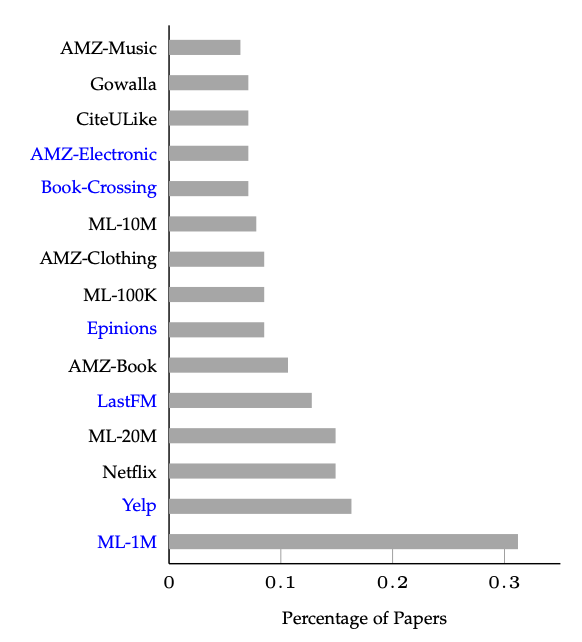
\includegraphics[width=0.6\textwidth]{images/dataset_dist.png}
    \caption{Розподіл використання наборів даних у наукових статтях.}
\end{figure}
Для практичних еспериментів, а також навчання і валідації моделей будо обрано відкриті набори даних які є загально прийняті і використовуються для порівняння у академічній сфері (Рис. 6.1). Для кожного датасету проведений розвідувальний аналіз даних (EDA) для оприділення їх основних структурних особливостей і відмінностей. Кожен набір є зрізом БД приватних комерційних компаній, тому можна вважати що поведінка моделей відповідає реальним результатам.

\subsubsection{Movielens 1M}
Набір даних Movielens (ML-1M) є найпопулярнішим серед великого різноманіття датасетів. Movielens -  це мережева система рекомендацій фільмів для користувачів на базі їх відгуків і оцінок. Існує із 1996 року і містить у собі більше 11 мільйонів оцінок для 8600 об’єктів.
\begin{figure}[H]
    \centering
    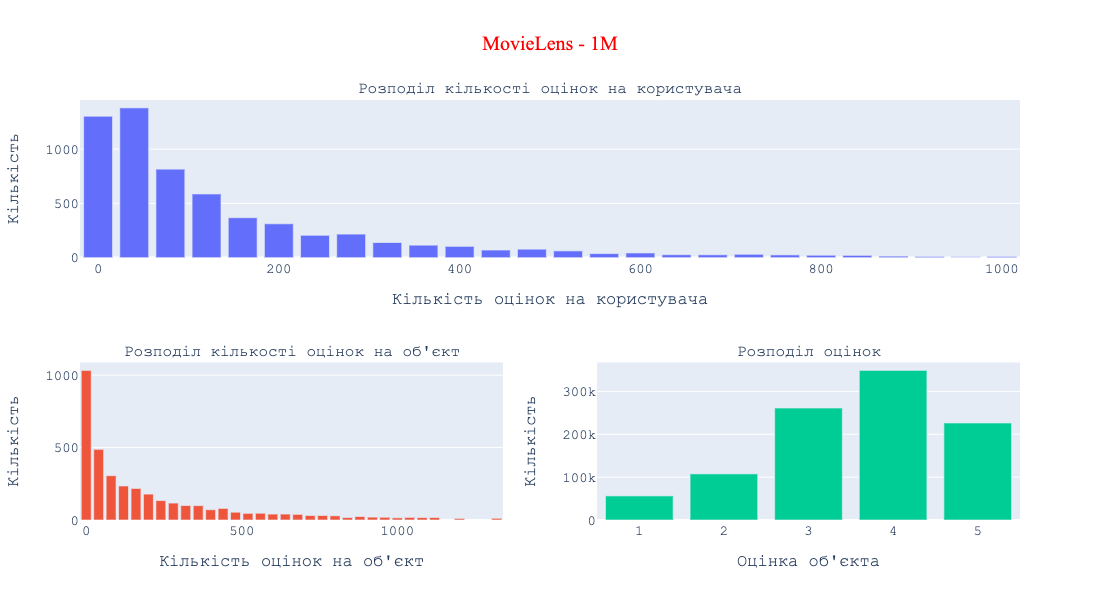
\includegraphics[width = 1\textwidth]{images/ML-1m_stat.png}    
    \caption{EDA для набору даних Movielens (ML-1M) }
\end{figure}
Структура набору наступна: 
\begin{itemize}
    \item $item\_id$ індентифікатор користувача.
    \item $user\_id$ індентифікатор об’єкта рекомендацій.
    \item $score$ оцінка.
    \item $timestamp$ дата і час дії.
\end{itemize}

Для аналізу відібрано 3706 об’єктів рекомендацій (фільмів) із 1 000 036  оцінок від корисутувачів. Що надає не менше 20 відгуків на один об’єкт.
\begin{table}[H]
    \centering
    \caption{Характеристика набору даних Movielens 1M}
    \begin{tabular}{|c|c|}
        \hline
        Загальна статистика      & Значення \\ \hline
        Кількість взаємодій      & 1 000 029                    \\
        Кількість користувачів   & 6 040                        \\
        Кількість об’єктів       & 3 706                        \\
        Розрідженність           & 99.9553\%                    \\
        Середня оцінка           & 3.58 / 5                     \\ \hline
        Взаємодій на користувача &                              \\ \hline
        Середнє                  & 165.6                        \\
        Медіана                  & 96.0                         \\ \hline
        Взаємодій на об’єкт      &                              \\ \hline
        Середнє                  & 269.89                       \\
        Медіана                  & 123.5                        \\ \hline
    \end{tabular}
    \label{tab:ML-1m}
\end{table}
Більшість оцінок приймають значення від 3 до 4-5. У розподілі взаємодій чітко замітний лівий перекіс, що типово для даних такого роду. Розрідженість висока.


\subsubsection{LastFm}
Набір даних LastFm містить у собі інформацію про музику яка прослуховується у медіа плеєрах користувачів. Структурно датасет подібний до ML-1M, але додатково присутня інформація про ключові теги класу для об’єктів. Теги можуть описувати жанр, автора, додаткову ключову інформацію, що є зручним і може бути використано для насичення моделей.


\begin{figure}[H]
    \centering
    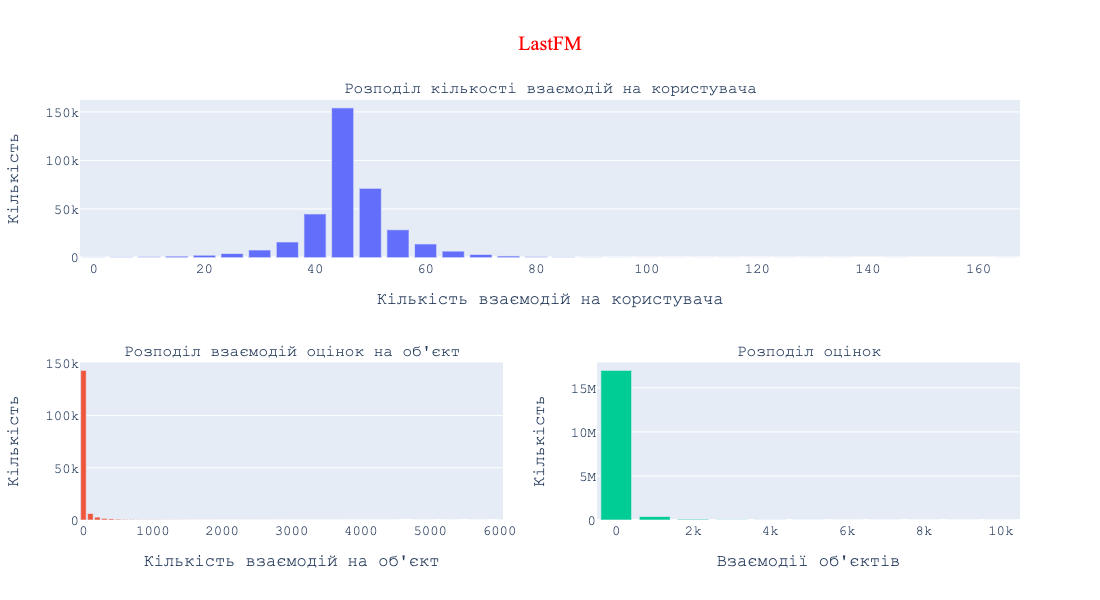
\includegraphics[width = 1\textwidth]{images/LastFM_stat.png}    
    \caption{EDA для набору даних Last.fm}
\end{figure}

\begin{table}[H]
    \centering
    \caption{Характеристика набору даних LastFM}
    \begin{tabular}{|c|c|}
        \hline
        Загальна статистика      & Значення \\ \hline
        Кількість взаємодій      & 17 535 654                    \\
        Кількість користувачів   & 358 868                        \\
        Кількість об’єктів       & 160 113                        \\
        Розрідженність           & 99.9996\%                    \\\hline
        Взаємодій на користувача &                              \\ \hline
        Середнє                  & 48.23                        \\
        Медіана                  & 48.0                         \\ \hline
        Взаємодій на об’єкт      &                              \\ \hline
        Середнє                  & 108.10                       \\
        Медіана                  & 6.0                        \\ \hline
    \end{tabular}

    \label{tab:LastFM}
\end{table}

\subsubsection{Netflix}
Набір даних Netflix є одним із найбільших відкритих датасетів із реальними даними. Набір був створений під егідою проведення змагання Netflix Prize. Ціллю якого було розробка системи рекомендацій, переможець який добився найвищих показників якості отримав призову винагороду у розмірі 1 мільйон доларів. Датасет має класичну структуру: включає у собі дані про оцінки користувачів фільмів які були переглянути користувачами. Для кожного екземпляру є відмітка про час оцінки. 

Дані мають типовий розподіл, і явно замітний перекіс. Із цікавого, через великий розмір і характер домену (рекомендація фільмів), датасет є одним із найнасичених. Розподіл оцінок - стандартний ([3, 4, 5]). Більше 90\% користувачів оцінили менше ста об’єктів.
\begin{figure}[H]
    \centering
    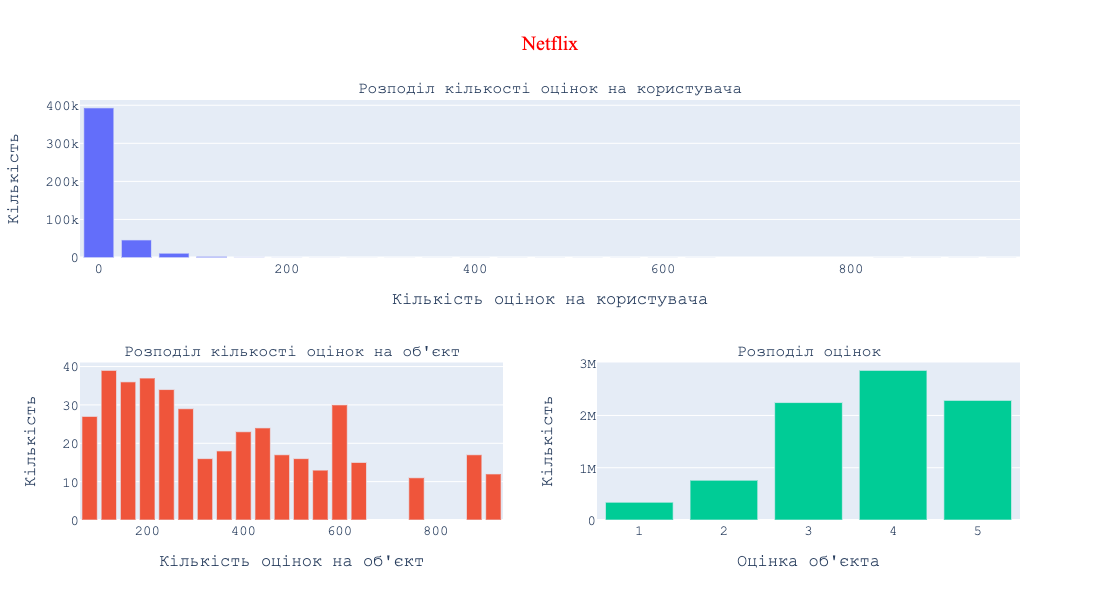
\includegraphics[width = 1\textwidth]{images/netflix_stat.png}    
    \caption{EDA для набору даних Netflix}
\end{figure}
У Таблиці 6.3 наведено докладна характеристика набору.
\begin{table}[H]
    \centering
    \caption{Характеристика набору даних Netflix}
    \begin{tabular}{|c|c|}
        \hline
        Загальна статистика      & Значення \\ \hline
        Кількість взаємодій      & 100 480 507                  \\
        Кількість користувачів   & 480 189                        \\
        Кількість об’єктів       & 17 770                        \\
        Розрідженність           & 98.8239\%                    \\\hline
        Взаємодій на користувача &                              \\ \hline
        Середнє                  & 209.33                       \\
        Медіана                  & 87.0                         \\ \hline
        Взаємодій на об’єкт      &                              \\ \hline
        Середнє                  & 5654.50                       \\
        Медіана                  & 967                      \\ \hline
    \end{tabular}
    \label{tab:Netflix}
\end{table}

Середня кількісь оцінок на об’єкт є надзвичайно високою.
\subsection{Середовище розгортання}

Експермиментальне дослідження проводиться на базі сервісу хмарних обчислень  Google Colab. Для навчання використано GPU Nvidia Tesla K80. Дані датасетів отримані із офіційних сторінок, розміщені у хмарному сховищі у вигляді текстових документів. Версія Python 3.8.15. Моделі імплементовані із використпанням бібліотеки torch. 

% Проведений аналіз наборів даних для побудови рекомендацій. Оцінено їх насиченість, частоту взаємодій відносно користувача і об’єкту. Наведено справочну інформацію про розмір, об’єм і структуру наборів. Вказано платформу реалізації практичних експериментів.

\subsection{Результати дослідження}
На основі аналізу факторів впливу, а також розглянутих перспективних нейромережевих моделей побудови рекомендацій було сформовано набір експериментів (Таблиця 8.1). Завдання експериментів, використовуючи набори даних, які відповідають реальним вибіркам із БД комерційних компаній дослідити вплив широкого спектру розглянутих факторів. Використовуючи мову програмування Python, а також платформу хмарних обчислень Google Coolab імплементувано розглянуті алгоритми Neural Matrix Factorization, Variational AutoEncoder ,  Neural Graph Colaborative Filtering.

На основі імплементованих алгоритмів проведений порівняльний аналіз ефективності використовуючи метрики вказані у Таблиці 8.1 . 
% Провести пошук оптимальних гіперпараметрів для алгоритмів. Розглянути еффективіність методів:
% \begin{itemize}
%     \item Сплітингу
%     \item Семплювання
%     \item Ініціалізації гіперпараметрів
%     \item Оптимізації
%     \item Регуляризації
% \end{itemize}

% \begin{table}[h]
%     \caption{}
%     \begin{tabular}{|c|c|}
%         \hline
%         Фактор                 & Значення                                                                                   \\ \hline
%         Датасет                & ML-1m, LastFM, Netflix                                                                     \\ \hline
%         Модель                 & NeuMF, VAE, NGCF                                                                           \\ \hline
%         Фільтрація датасету    & Без фільтрації, 5, 10                                                                      \\ \hline
%         Сплітінг датасету      & За пропорціями, За часом                                                                   \\ \hline
%         Метрик оцінки якості   & \begin{tabular}[c]{@{}c@{}}Precision@k, Recall@k, MAP, HitRatio, MRR, \\ NDCG\end{tabular} \\ \hline
%         Семплювання            & Розподіл Гауса, low popularity, high popularity                                            \\ \hline
%         Ініціалізація $\theta$ & Рівномірний розподіл, Розподіл Гауса                                                       \\ \hline
%         Метод оптимізації      & GD, SGD, BSGD, AdaGrad, RMSProp                                                            \\ \hline
%         Регуляризація          &                                                                                            \\ \hline
%         Підбір гіперпараметрів & GridSearch, Bayesian HyperOpt                                                              \\ \hline
%     \end{tabular}
%     \label{tab:Expr_design}
% \end{table}

\begin{table}[h]
    \caption{Деталі експерименту}
    \begin{tabular}{|c|c|}
        \hline
        Фактор                 & Значення                                                                                   \\ \hline
        Датасет                & ML-1m, LastFM, Netflix                                                                     \\ \hline
        Модель                 & NeuMF, VAE, NGCF                                                                           \\ \hline
        Фільтрація датасету    & Без фільтрації                              \\ \hline
        Сплітінг датасету      & За часом                                                                   \\ \hline
        Метрик оцінки якості   & \begin{tabular}[c]{@{}c@{}}Precision@k, Recall@k, MAP, HitRatio, MRR, \\ NDCG\end{tabular} \\ \hline
        Семплювання            & Розподіл Гауса                                            \\ \hline
        Ініціалізація $\theta$ &  Розподіл Гауса                                                       \\ \hline
        Метод оптимізації      &  AdaGrad                                                             \\ \hline
        Регуляризація          &  L2                                                                                          \\ \hline
        Підбір гіперпараметрів & GridSearch                                                              \\ \hline
    \end{tabular}
    \label{tab:Expr_design}
\end{table}
Значення функцій втрат під час навчання для кожного із алгоритмів вказано на Рис. 8.1. Для NeuMF  було застосовано ранню зупинку, loss не змінювався протягом 3 епох. Дельта втрат вказує на рівномірне зменшування функції втрат.
Для MultiVAE доцільно використати сильнішу регуляризацію. 
\begin{figure}
    \begin{subfigure}{\textwidth}
        \centering
        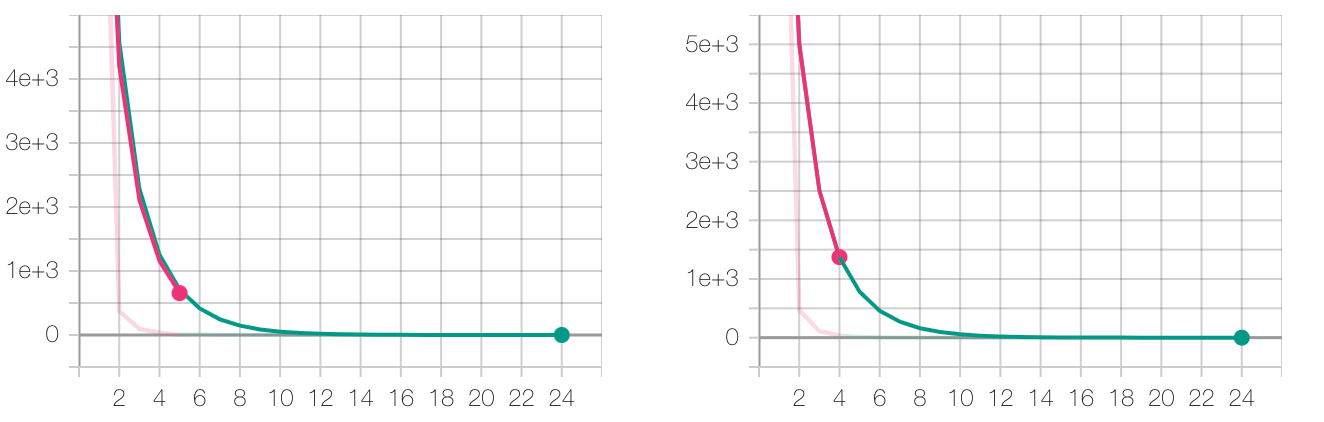
\includegraphics[width=.5\textwidth]{images/experiments/neumf_loss.png}
        \caption{Навчання NeuMF на 24 епохах}
    \end{subfigure}
    \begin{subfigure}{\textwidth}
        \centering
        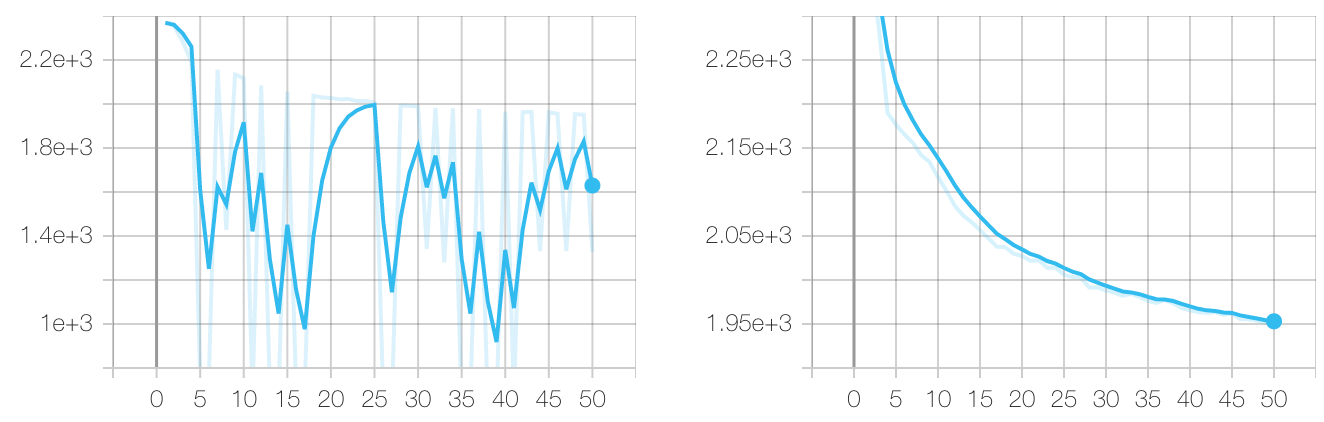
\includegraphics[width=.5\textwidth]{images/experiments/multivae_loss.png}
        \caption{Навчання MultiVae на 50 епохах}
    \end{subfigure}
    \begin{subfigure}{\textwidth}
        \centering
        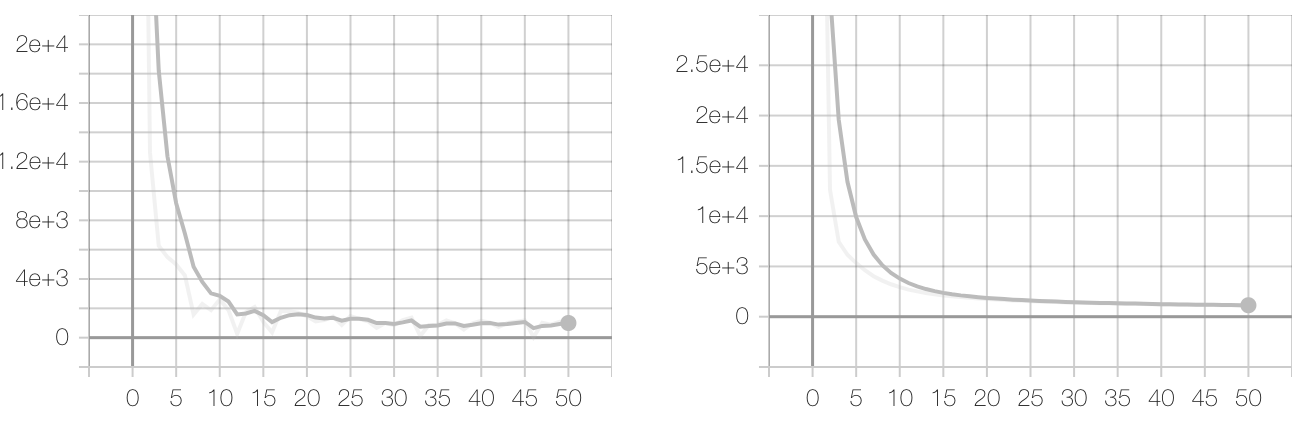
\includegraphics[width=.5\textwidth]{images/experiments/ngcd_loss.png}
        \caption{Навчання NGCF на 50 епохах}
    \end{subfigure}
    \caption{Процес навчання алгоритмів. Зправа - Значення функції втрат, Зліва - дельта втрат відносно епохи.}
\end{figure}
У наступних таблицях вказано результи метри якості розраховані на наборі даних Movielens.  K (розмір списку рекомендацій) був обраний із інтервалу [1, 50].
Для розрахунку бува використане негативне семплювання, із розміро вибірки 1000 у кандидатів.
\begin{table}
    \centering
    \begin{tabular}{|l|l|l|l|l|l|l|}
        \hline
        KPI@K     & 1       & 5       & 10     & 20     & 30     & 50     \\ \hline
        Recall    & 0.01452 & 0.06699 & 0.1235 & 0.2215 & 0.3012 & 0.4135 \\ \hline
        MRR       & 0.6961  & 0.7929  & 0.79   & 0.7981 & 0.7983 & 0.7985 \\ \hline
        NDCG      & 0.6961  & 0.8175  & 0.8200 & 0.8112 & 0.8050 & 0.7978 \\ \hline
        Hit Ratio & 0.6961  & 0.9246  & 0.9584 & 0.9636 & 0.9688 & 0.9766 \\ \hline
        Precision & 0.6961  & 0.641   & 0.5906 & 0.5302 & 0.4785 & 0.3966 \\ \hline
    \end{tabular}
    \caption{Значення метрик якості для алгоритму MultiVAE. Набір даних MovieLens}
\end{table}
\begin{table}
    \begin{tabular}{|l|l|l|l|l|l|l|}
        \hline
        KPI@K     & 1        & 5        & 10      & 20      & 30      & 50      \\ \hline
        Recall    & 0.001757 & 0.008701 & 0.01956 & 0.02799 & 0.04172 & 0.05583 \\ \hline
        MRR       & 0.04318  & 0.07580  & 0.0839  & 0.0901  & 0.09206 & 0.0941  \\ \hline
        NDCG      & 0.04318  & 0.08929  & 0.1087  & 0.1315  & 0.1407  & 0.157   \\ \hline
        Hit Ratio & 0.04318  & 0.1295   & 0.1926  & 0.2823  & 0.3322  & 0.4086  \\ \hline
        Precision & 0.04318  & 0.04518  & 0.04186 & 0.03787 & 0.03665 & 0.03342 \\ \hline
    \end{tabular}
    \caption{Значення метрик якості для алгоритму NGCF. Набір даних MovieLens}
\end{table}
\begin{table}
    \begin{tabular}{|l|l|l|l|l|l|l|}
        \hline
        KPI@K     & 1        & 5       & 10      & 20      & 30     & 50      \\ \hline
        Recall    & 0.003363 & 0.01157 & 0.02017 & 0.04535 & 0.0611 & 0.09025 \\ \hline
        MRR       & 0.1694   & 0.2382  & 0.2603  & 0.2688  & 0.2717 & 0.2732  \\ \hline
        NDCG      & 0.1694   & 0.2688  & 0.322   & 0.354   & 0.3701 & 0.381   \\ \hline
        Hit Ratio & 0.1694   & 0.365   & 0.5348  & 0.657   & 0.73   & 0.7873  \\ \hline
        Precision & 0.1694   & 0.1408  & 0.1355  & 0.1250  & 0.119  & 0.1136  \\ \hline
    \end{tabular}
    \caption{Значення метрик якості для алгоритму NeuMF. Набір даних MovieLens}
\end{table}

\begin{figure}[H]
    \centering
    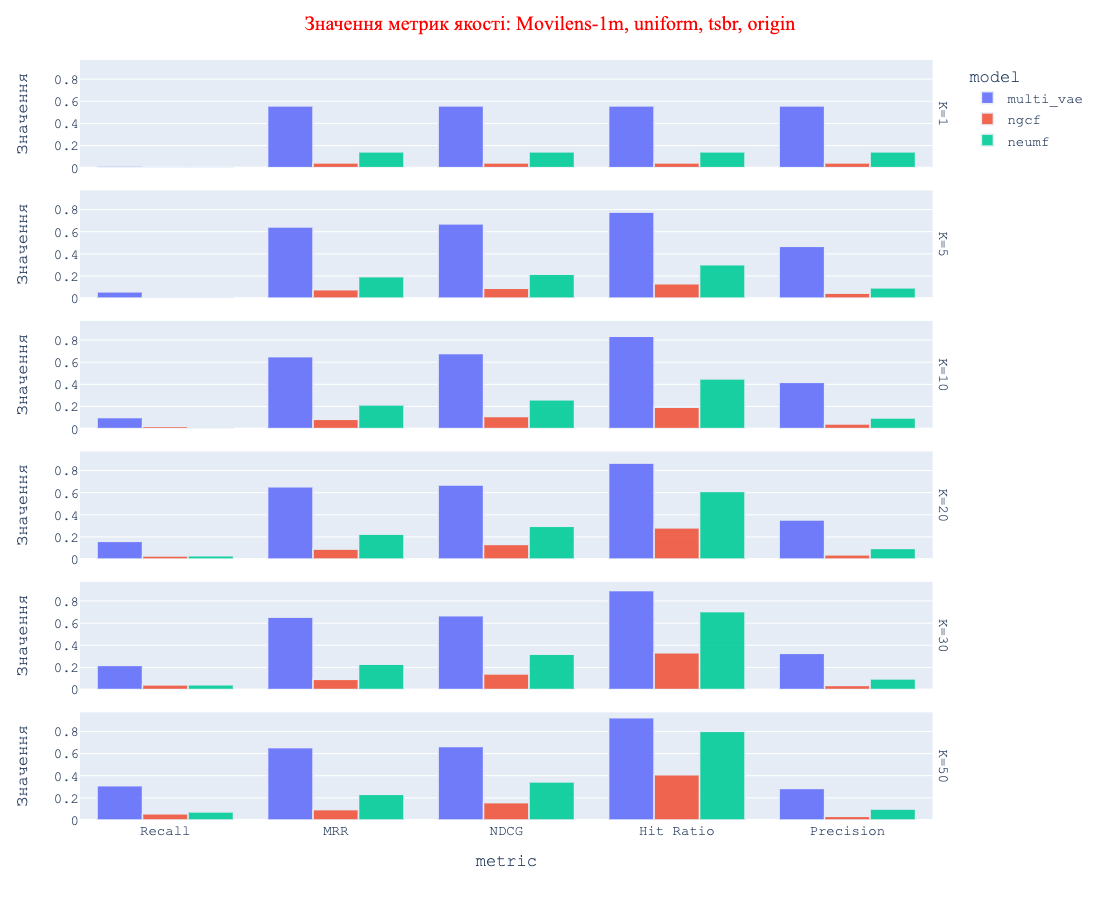
\includegraphics[width=1\textwidth]{images/experiments/metrics_exp_1.png}
    \caption{Порівняльний графік метрик якості}
\end{figure}

Алгоритм MultiVae  показав найвищі показники метрик якості на усіх вибірках K,. Варіаційний автоенкодер показує потужну властивість до вивчення поведінки користувачів.


\subsection*{Висновки}
Було проведено експерементальне дослідження здатності до побудови рекомендацій алгоритмів NueMF, MultiVAE і NGCF. За результатами тестування,  MultiVAE  показав найвищі результати по всім розглянутим метрикам.
\newpage
\section{ВИСНОВКИ}
\subsection{Наукова новизна отриманих результатів}
Враховуючи результати експерементів було знайдено ключові фактори впливу на якість та ефективність роботи моделей  глибокого навчання у системах рекомендацій.
Розроблений алгоритм дає можливість прискорити прототипування, перевірку і порівняння існуючих та майбутніх моделей систем рекомендацій.
\subsection{Практичне значення отриманих результатів}
Було сформульовано і змодельовано наступні фактори впливу 
\begin{enumerate}
    \item Вибір спліт методу. Методу  Dataset Spliting Method
    \item Вибір метрики якості Evaluation Metric Selection
    \item Формулювання функції втрат для оптимізації Loss function Design
    \item Мотодологія негативного семплінгу. Негативний Negative Samoling Strategy
    \item Стратегія ініціалізації вагів. Parap Init Strategy
    \item Вибір алгоритму оптимізації Model Optimizer Selection 
    \item Вибір методу регуляризації Regularization Term /  Dropout
    \item Критерії останова Early Stop Mechanism
    \item Донавчання вагів Hyper Params Tuning
    \end{enumerate}
Проведене експерементальне дослідження їх впливу на якість роботи  обраних алгоритмів рекомендацій. 
Розроблене ПЗ пришвидшує відбір оптимальних моделей і їх якісне порівняння. ПЗ може використовуватись як і для комерційних цілей так і (наукових) для порівняння нових алгоритмів.

У даній роботі було проаналізовано задачу побудови рекомендацій, розглянуто її проблематику. Розглянуто широкий спектр метрик якості із використанням підходу до класифікації, ранжування і різноманіття.
На основі алгоритмів нейромережевої факторизації, варіаційного автоенкодера і графової нейронної колаборативної фільтрації було розглянуто підхід глибокого навчання до побудови рекомендацій.
Сформовано перелік факторів впливу на метрики якості. Проведений аналіз їх впливу і можливі рішення для усунення.
На основі відкритих наборів даних було імплементовано розглянуті алгоритми рекомендації і проведене їх порівняння.


\newpage
\begin{thebibliography}{99}
    \bibitem{NEUMF}
    Xiangnan He, Lizi Liao, Hanwang Zhang, Liqiang Nie, Xia Hu, and Tat-Seng Chua. 2017.  \emph{Neural Collaborative Filtering}. In Proceedings of the 26th International Conference on World Wide Web (WWW '17). International World Wide Web Conferences Steering Committee, Republic and Canton of Geneva, CHE, 173–182. https://doi.org/10.1145/3038912.3052569
    \bibitem{VAE}
    Dawen Liang, Rahul G. Krishnan, Matthew D. Hoffman, and Tony Jebara. 2018. \emph{Variational Autoencoders for Collaborative Filtering}. In Proceedings of the 2018 World Wide Web Conference (WWW '18). International World Wide Web Conferences Steering Committee, Republic and Canton of Geneva, CHE, 689–698. https://doi.org/10.1145/3178876.3186150
    \bibitem{NGCF}
    Xiang Wang, Xiangnan He, Meng Wang, Fuli Feng, and Tat-Seng Chua. 2019. \emph{Neural Graph Collaborative Filtering}. In Proceedings of the 42nd International ACM SIGIR Conference on Research and Development in Information Retrieval (SIGIR'19). Association for Computing Machinery, New York, NY, USA, 165–174. https://doi.org/10.1145/3331184.3331267
    \bibitem{GraphBook}
    William L. Hamilton. (2020). \emph{Graph Representation Learning}. Synthesis Lectures on Artificial Intelligence and Machine Learning, Vol. 14, No. 3 , Pages 1-159.
    \bibitem{MetaRec}
    Le, James, "MetaRec: Meta-Learning Meets Recommendation Systems" (2020). Thesis. Rochester Institute of Technology.
    \bibitem{Metrics}
    Saúl Vargas. 2014. \emph{Novelty and diversity enhancement and evaluation in recommender systems and information retrieval}. In Proceedings of the 37th international ACM SIGIR conference on Research  development in information retrieval (SIGIR '14). Association for Computing Machinery, New York, NY, USA, 1281. https://doi.org/10.1145/2600428.2610382
    \bibitem{MetricPtoblems}
    Zhu Sun, Di Yu, Hui Fang, Jie Yang, Xinghua Qu, Jie Zhang, and Cong Geng. 2020. \emph{Are We Evaluating Rigorously? Benchmarking Recommendation for Reproducible Evaluation and Fair Comparison}. In Proceedings of the 14th ACM Conference on Recommender Systems (RecSys '20). Association for Computing Machinery, New York, NY, USA, 23–32. https://doi.org/10.1145/3383313.3412489
    \bibitem{RecoBook}
    Francesco Ricci, Lior Rokach, Bracha Shapira, and Paul B. Kantor. 2010. \emph{Recommender Systems Handbook (1st. ed.)}. Springer-Verlag, Berlin, Heidelberg.
    \bibitem{Bishop}
    Christopher M. Bishop. \emph{Pattern Recognition and Machine Learning}. 2006. ISBN-10: 0-387-31073-8. Springer New York, NY
    \bibitem{Colab}
    Google Colab [Електронний ресурс]. – Режим доступу:\href{https://colab.research.google.com/}{https://colab.research.google.com/}
    \bibitem{NetflixDataset}
    Netflix Prize Dataset [Електронний ресурс]. – Режим доступу:\href{https://archive.org/download/nfprize_dataset.tar}{https://archive.org/download/nfprize\_dataset.tar}
    \bibitem{MovilensDataset}
    Movilens Dataset [Електронний ресурс]. – Режим доступу:\href{https://grouplens.org/datasets/movielens/1m/}{https://grouplens.org/datasets/movielens/1m/}
    \bibitem{LastFMDataset}
    LastFM Dataset [Електронний ресурс]. – Режим доступу:\href{https://grouplens.org/datasets/hetrec-2011/}{https://grouplens.org/datasets/hetrec-2011/}
    \bibitem{Perceptron}
    Персептрон [Електронний ресурс]. – Режим доступу:\href{https://ru.wikipedia.org/wiki/%D0%9F%D0%B5%D1%80%D1%86%D0%B5%D0%BF%D1%82%D1%80%D0%BE%D0%BD}{https://ru.wikipedia.org/wiki/Перцептрон}
    \end{thebibliography}
% \newpage
% \section{ДОДАТКИ}
% Код проведення експериментів.
% \centering
% \begin{lstlisting}[language=Python,breaklines]

% import os
% from tqdm import tqdm
% import torch
% import torch.nn as nn
% import torch.optim as optim

% from utils.loss import BPRLoss, TOP1Loss, HingeLoss


% class AbstractRecommender(nn.Module):
%     def __init__(self):
%         super(AbstractRecommender, self).__init__()
%         self.optimizer = None
%         self.initializer = None
%         self.loss_type = None
%         self.lr = 0.01
%         self.logger = None

%         self.initializer_param_config = {
%             'normal': {'mean':0.0, 'std':0.01},
%             'uniform': {'a':0.0, 'b':1.0},
%             'xavier_normal': {'gain':1.0},
%             'xavier_uniform': {'gain':1.0}
%         }

%         self.initializer_config = {
%             'normal': nn.init.normal_,
%             'uniform': nn.init.uniform_,
%             'xavier_normal': nn.init.xavier_normal_,
%             'xavier_uniform': nn.init.xavier_uniform_
%         }

%     def calc_loss(self, batch):
%         raise NotImplementedError

%     def fit(self, train_loader):
%         raise NotImplementedError

%     def rank(self, test_loader):
%         raise NotImplementedError

%     def full_rank(self, u):
%         raise NotImplementedError

%     def predict(self, u, i):
%         raise NotImplementedError

%     def _build_optimizer(self, **kwargs):
%         params = self.parameters()
%         learner = kwargs.pop('optimizer', self.optimizer)
%         learning_rate = kwargs.pop('lr', self.lr)

%         if learner.lower() == 'adam':
%             optimizer = optim.Adam(params, lr=learning_rate)
%         elif learner.lower() == 'sgd':
%             optimizer = optim.SGD(params, lr=learning_rate)
%         elif learner.lower() == 'adagrad':
%             optimizer = optim.Adagrad(params, lr=learning_rate)
%         elif learner.lower() == 'rmsprop':
%             optimizer = optim.RMSprop(params, lr=learning_rate)
%         elif learner.lower() == 'sparse_adam':
%             optimizer = optim.SparseAdam(params, lr=learning_rate)
%         else:
%             self.logger.info('Received unrecognized optimizer, set default Adam optimizer')
%             optimizer = optim.Adam(params, lr=learning_rate)

%         return optimizer

%     def _init_weight(self, m):
%         if isinstance(m, nn.Linear):
%             self.initializer_config[self.initializer](m.weight, **self.initializer_param_config[self.initializer])
%             if m.bias is not None:
%                 nn.init.constant_(m.bias.data, 0.)
%         elif isinstance(m, nn.Embedding):
%             self.initializer_config[self.initializer](m.weight, **self.initializer_param_config[self.initializer])
%         else:
%             pass

%     def _build_criterion(self, loss_type):
%         if loss_type.upper() == 'CL':
%             criterion = nn.BCEWithLogitsLoss(reduction='sum')
%         elif loss_type.upper() == 'SL':
%             criterion = nn.MSELoss(reduction='sum')
%         elif loss_type.upper() == 'BPR':
%             criterion = BPRLoss()
%         elif loss_type.upper() == 'HL':
%             criterion = HingeLoss()
%         elif loss_type.upper() == 'TL':
%             criterion = TOP1Loss()
%         else:
%             raise NotImplementedError(f'Invalid loss type: {self.loss_type}...')

%         return criterion

% class GeneralRecommender(AbstractRecommender):
%     def __init__(self, config):
%         super(GeneralRecommender, self).__init__()

%         os.environ['CUDA_VISIBLE_DEVICES'] = config['gpu']
%         self.device = 'cuda' if torch.cuda.is_available() else 'cpu'
%         self.logger = config['logger']

%     def fit(self, train_loader):
%         self.to(self.device)
%         optimizer = self._build_optimizer(optimizer=self.optimizer, lr=self.lr)
%         if self.loss_type is not None:
%             self.criterion = self._build_criterion(self.loss_type)
%         else:
%             self.criterion = None

%         last_loss = 0.
%         for epoch in range(1, self.epochs + 1):
%             self.train()

%             current_loss = 0.
%             pbar = tqdm(train_loader)
%             pbar.set_description(f'[Epoch {epoch:03d}]')
%             for batch in pbar:
%                 self.zero_grad()
%                 loss = self.calc_loss(batch)

%                 if torch.isnan(loss):
%                     raise ValueError(f'Loss=Nan or Infinity: current settings does not fit the recommender')

%                 loss.backward()
%                 optimizer.step()

%                 current_loss += loss.item()
%             pbar.set_postfix(loss=current_loss)

%             self.eval()
%             delta_loss = float(current_loss - last_loss)
%             if (abs(delta_loss) < 1e-5) and self.early_stop:
%                 self.logger.info('Satisfy early stop mechanism')
%                 break
%             else:
%                 last_loss = current_loss

% class AERecommender(GeneralRecommender):
%     def __init__(self, config):
%         super(AERecommender, self).__init__(config)
%         self.user_num = None 
%         self.item_num = None
%         self.history_user_id, self.history_item_id = None, None
%         self.history_user_value, self.history_item_value = None, None

%     def get_user_rating_matrix(self, user):
%         '''
%         just convert the raw rating matrix to a much smaller matrix for calculation,
%         the row index will be the new id for uid, but col index will still remain the old iid
%         '''
%         col_indices = self.history_item_id[user].flatten() # batch * max_inter_by_user -> (batch * max_inter_by_user)
%         row_indices = torch.arange(user.shape[0]).to(self.device).repeat_interleave(
%             self.history_item_id.shape[1], dim=0) # batch -> (batch * max_inter_by_user)
%         rating_matrix = torch.zeros(1).to(self.device).repeat(user.shape[0], self.item_num) # batch * item_num
%         rating_matrix.index_put_((row_indices, col_indices), self.history_item_value[user].flatten())
        
%         return rating_matrix

%     def get_item_rating_matrix(self, item):
%         col_indices = self.history_user_id[item].flatten()
%         row_indices = torch.arange(item.shape[0]).to(self.device).repeat_interleave(
%             self.history_user_id.shape[1], dim=0)
%         rating_matrix = torch.zeros(1).to(self.device).repeat(item.shape[0], self.user_num)
%         rating_matrix.index_put_((row_indices, col_indices), self.history_user_value[item].flatten())
        
%         return rating_matrix


% import torch
% import torch.nn as nn
% import torch.nn.functional as F

% import numpy as np
% import scipy.sparse as sp

% from model.AbstractRecommender import GeneralRecommender

% class SparseDropout(nn.Module):
%     '''
%     This is a Module that execute Dropout on Pytorch sparse tensor.
%     '''
%     def __init__(self, p=0.5):
%         super(SparseDropout, self).__init__()
%         # p is ratio of dropout
%         # convert to keep probability
%         self.kprob = 1 - p

%     def forward(self, x):
%         if not self.training:
%             return x

%         mask = ((torch.rand(x._values().size()) + self.kprob).floor()).type(torch.bool)
%         rc = x._indices()[:, mask]
%         val = x._values()[mask] * (1.0 / self.kprob)
%         return torch.sparse.FloatTensor(rc, val, x.shape)

% class BiGNN(nn.Module):
%     '''
%     Propagate a layer of Bi-interaction GNN
%         L = D^-1(A)D^-1 is laplace matrix, I is identity matrix
%         output = (L+I)EW_1 + LE \otimes EW_2 = (LE + E)W_1 + LE \otimes EW_2
%         so I can be never used.
%     '''

%     def __init__(self, in_dim, out_dim):
%         super(BiGNN, self).__init__()
%         self.in_dim = in_dim
%         self.out_dim = out_dim
%         self.linear = torch.nn.Linear(in_features=in_dim, out_features=out_dim)
%         self.interact_transform = torch.nn.Linear(in_features=in_dim, out_features=out_dim)

%     def forward(self, lap_matrix, features):
%         x = torch.sparse.mm(lap_matrix, features)

%         inter_part1 = self.linear(features + x)
%         inter_feature = torch.mul(x, features)
%         inter_part2 = self.interact_transform(inter_feature)

%         return inter_part1 + inter_part2

% class NGCF(GeneralRecommender):
%     def __init__(self, config):
%         """
%         NGCF Recommender Class
%         Parameters
%         ----------
%         user_num : int, the number of users
%         item_num : int, the number of items
%         factors : int, the number of latent factor
%         node_dropout: float, node dropout ratio
%         mess_dropout : float, messsage dropout rate
%         hidden_size_list : list, dimension structure of hidden layers, optional.
%         lr : float, learning rate
%         reg_1 : float, first-order regularization term
%         reg_2 : float, second-order regularization term
%         epochs : int, number of training epochs
%         loss_type : str, loss function type
%         gpuid : str, GPU ID
%         early_stop : bool, whether to activate early stop mechanism
%         """
%         super(NGCF, self).__init__(config)

%         self.epochs = config['epochs']
%         self.lr = config['lr']
%         self.topk = config['topk']
%         self.user_num = config['user_num']
%         self.item_num = config['item_num']

%         # get this matrix from utils.get_inter_matrix and add it in config
%         self.interaction_matrix = config['inter_matrix']

%         self.embedding_size = config['factors']
%         self.hidden_size_list = config["hidden_size_list"] if config['hidden_size_list'] is not None else [64, 64, 64]
%         self.hidden_size_list = [self.embedding_size] + self.hidden_size_list

%         self.node_dropout = config['node_dropout']
%         self.message_dropout = config['mess_dropout']
%         self.reg_1 = config['reg_1']
%         self.reg_2 = config['reg_2']

%         self.sparse_dropout = SparseDropout(self.node_dropout)
%         self.embed_user = nn.Embedding(self.user_num, self.embedding_size)
%         self.embed_item = nn.Embedding(self.item_num, self.embedding_size)
%         self.gnn_layers = torch.nn.ModuleList()
%         for _, (in_size, out_size) in enumerate(zip(self.hidden_size_list[:-1], self.hidden_size_list[1:])):
%             self.gnn_layers.append(BiGNN(in_size, out_size))
        
%         # storage variables for evaluation acceleration
%         self.restore_user_e = None
%         self.restore_item_e = None

%         self.loss_type = config['loss_type']
%         self.optimizer = config['optimizer'] if config['optimizer'] != 'default' else 'adam'
%         self.initializer = config['init_method'] if config['init_method'] != 'default' else 'xavier_normal'
%         self.early_stop = config['early_stop']

%         # parameters initialization
%         self.apply(self._init_weight)

%         self.norm_adj_matrix = self.get_norm_adj_mat().to(self.device)
%         # self.eye_matrix = self.get_eye_mat().to(self.device)

%     def get_norm_adj_mat(self):
%         A = sp.dok_matrix((self.user_num + self.item_num, self.user_num + self.item_num), dtype=np.float32)
%         inter_M = self.interaction_matrix
%         inter_M_t = self.interaction_matrix.transpose()
%         data_dict = dict(zip(zip(inter_M.row, inter_M.col + self.user_num), [1] * inter_M.nnz))
%         data_dict.update(dict(zip(zip(inter_M_t.row + self.user_num, inter_M_t.col), [1] * inter_M_t.nnz)))
%         A._update(data_dict)
%         # norm adj matrix
%         sum_arr = (A > 0).sum(axis=1)
%         diag = np.array(sum_arr.flatten())[0] + 1e-7  # add epsilon to avoid divide by zero Warning
%         diag = np.power(diag, -0.5)
%         D = sp.diags(diag)
%         L = D * A * D
%         # covert norm_adj matrix to tensor
%         L = sp.coo_matrix(L)
%         row = L.row
%         col = L.col
%         i = torch.LongTensor(np.array([row, col]))
%         data = torch.FloatTensor(L.data)
%         SparseL = torch.sparse.FloatTensor(i, data, torch.Size(L.shape))
%         return SparseL

%     def get_eye_mat(self):
%         num = self.user_num + self.item_num  # number of column of the square matrix
%         i = torch.LongTensor([range(0, num), range(0, num)])
%         val = torch.FloatTensor([1] * num)  # identity matrix
%         return torch.sparse.FloatTensor(i, val)

%     def get_ego_embeddings(self):
%         user_embeddings = self.embed_user.weight
%         item_embeddings = self.embed_item.weight
%         ego_embeddings = torch.cat([user_embeddings, item_embeddings], dim=0)
%         return ego_embeddings

%     def forward(self):
%         A_hat = self.sparse_dropout(self.norm_adj_matrix) if self.node_dropout != 0 else self.norm_adj_matrix
%         all_embeddings = self.get_ego_embeddings()
%         embeddings_list = [all_embeddings]
%         for gnn in self.gnn_layers:
%             all_embeddings = gnn(A_hat, all_embeddings)
%             all_embeddings = nn.LeakyReLU(negative_slope=0.2)(all_embeddings)
%             all_embeddings = nn.Dropout(self.message_dropout)(all_embeddings)
%             all_embeddings = F.normalize(all_embeddings, p=2, dim=1)
%             embeddings_list += [all_embeddings]  # storage output embedding of each layer
%         ngcf_all_embeddings = torch.cat(embeddings_list, dim=1)

%         user_all_embeddings, item_all_embeddings = torch.split(ngcf_all_embeddings, [self.user_num, self.item_num])

%         return user_all_embeddings, item_all_embeddings

%     def calc_loss(self, batch):
%         if self.restore_user_e is not None or self.restore_item_e is not None:
%             self.restore_user_e, self.restore_item_e = None, None

%         user = batch[0].to(self.device).long()
%         pos_item = batch[1].to(self.device).long()

%         embed_user, embed_item = self.forward()

%         u_embeddings = embed_user[user]
%         pos_embeddings = embed_item[pos_item]
%         pos_pred = torch.mul(u_embeddings, pos_embeddings).sum(dim=1)

%         u_ego_embeddings = self.embed_user(user)
%         pos_ego_embeddings = self.embed_item(pos_item)

%         if self.loss_type.upper() in ['CL', 'SL']:
%             label = batch[2].to(self.device).float()
%             loss = self.criterion(pos_pred, label)
%             # add regularization term
%             loss += self.reg_1 * (u_ego_embeddings.norm(p=1) + pos_ego_embeddings.norm(p=1))
%             loss += self.reg_2 * (u_ego_embeddings.norm() + pos_ego_embeddings.norm())
%         elif self.loss_type.upper() in ['BPR', 'TL', 'HL']:
%             neg_item = batch[2].to(self.device).long()
%             neg_embeddings = embed_item[neg_item]
%             neg_pred = torch.mul(u_embeddings, neg_embeddings).sum(dim=1)
%             neg_ego_embeddings = self.embed_item(neg_item)

%             loss = self.criterion(pos_pred, neg_pred)

%             loss += self.reg_1 * (u_ego_embeddings.norm(p=1) + pos_ego_embeddings.norm(p=1) + neg_ego_embeddings.norm(p=1))
%             loss += self.reg_2 * (u_ego_embeddings.norm() + pos_ego_embeddings.norm() + neg_ego_embeddings.norm())

%         else:
%             raise NotImplementedError(f'Invalid loss type: {self.loss_type}')

%         return loss

%     def predict(self, u, i):
%         if self.restore_user_e is None or self.restore_item_e is None:
%             self.restore_user_e, self.restore_item_e = self.forward()

%         u_embedding = self.restore_user_e[u]
%         i_embedding = self.restore_item_e[i]
%         pred = torch.matmul(u_embedding, i_embedding.t())

%         return pred.cpu().item()

%     def rank(self, test_loader):
%         if self.restore_user_e is None or self.restore_item_e is None:
%             self.restore_user_e, self.restore_item_e = self.forward()

%         rec_ids = torch.tensor([], device=self.device)

%         for us, cands_ids in test_loader:
%             us = us.to(self.device)
%             cands_ids = cands_ids.to(self.device)

%             user_emb = self.restore_user_e[us].unsqueeze(dim=1) # batch * 1 * factor
%             item_emb = self.restore_item_e[cands_ids].transpose(1, 2) # batch * factor * cand_num
%             scores = torch.bmm(user_emb, item_emb).squeeze() # batch * cand_num

%             rank_ids = torch.argsort(scores, descending=True)
%             rank_list = torch.gather(cands_ids, 1, rank_ids)
%             rank_list = rank_list[:, :self.topk]

%             rec_ids = torch.cat((rec_ids, rank_list), 0)

%         return rec_ids.cpu().numpy()

%     def full_rank(self, u):
%         if self.restore_user_e is None or self.restore_item_e is None:
%             self.restore_user_e, self.restore_item_e = self.forward()

%         user_emb = self.restore_user_e[u] # factor
%         items_emb = self.restore_item_e.data # item * factor
%         scores = torch.matmul(user_emb, items_emb.transpose(1, 0))

%         return torch.argsort(scores, descending=True)[:self.topk].cpu().numpy()

% import math
% import torch
% import torch.nn as nn
% import torch.nn.functional as F
% from model.AbstractRecommender import AERecommender


% class VAECF(AERecommender):
%     def __init__(self, config):
%         """
%         VAE Recommender Class
%         Parameters
%         ----------
%         mlp_hidden_size : List, Q-net dimension list
%         dropout : float, drop out rate
%         epochs : int, number of training epochs
%         lr : float, learning rate
%         latent_dim: size of bottleneck layer
%         anneal_cap : float, regularization for KLD
%         optimizer : str, optimization method for training the algorithms
%         initializer: str, parameter initializer
%         early_stop : bool, whether to activate early stop mechanism
%         """
%         super(VAECF, self).__init__(config)
%         self.epochs = config['epochs']
%         self.lr = config['lr']
%         self.dropout = config['dropout']

%         self.layers = config["mlp_hidden_size"] if config['mlp_hidden_size'] is not None else [600]
%         self.lat_dim = config['latent_dim']
%         self.anneal_cap = config['anneal_cap']
%         self.total_anneal_steps = config["total_anneal_steps"]

%         self.user_num = config['user_num']
%         self.item_num = config['item_num']

%         self.history_item_id = config['history_item_id'].to(self.device)
%         self.history_item_value = config['history_item_value'].to(self.device)
%         self.update = 0

%         self.encode_layer_dims = [self.item_num] + self.layers + [self.lat_dim]
%         self.decode_layer_dims = [int(self.lat_dim / 2)] + self.encode_layer_dims[::-1][1:]

%         self.encoder = self.mlp_layers(self.encode_layer_dims)
%         self.decoder = self.mlp_layers(self.decode_layer_dims)
        
%         self.optimizer = config['optimizer'] if config['optimizer'] != 'default' else 'adam'
%         self.initializer = config['init_method'] if config['init_method'] != 'default' else 'xavier_normal'
%         self.early_stop = config['early_stop']

%         self.apply(self._init_weight)
%         self.topk = config['topk']

%     def mlp_layers(self, layer_dims):
%         mlp_modules = []
%         for i, (in_dim, out_dim) in enumerate(zip(layer_dims[:-1], layer_dims[1:])):
%             mlp_modules.append(nn.Linear(in_dim, out_dim))
%             if i != len(layer_dims[:-1]) - 1:
%                 mlp_modules.append(nn.Tanh())
%         return nn.Sequential(*mlp_modules)

%     def reparameterize(self, mu, logvar):
%         if self.training:
%             std = torch.exp(0.5 * logvar)
%             eps = torch.randn_like(std)
%             return eps.mul(std).add_(mu)  # core calculation for predicting the real distribution
%         else:
%             return mu

%     def forward(self, rating_matrix):
%         h = F.normalize(rating_matrix)
%         h = F.dropout(h, self.dropout, training=self.training)
%         h = self.encoder(h)

%         mu = h[:, :int(self.lat_dim / 2)]
%         logvar = h[:, math.ceil(self.lat_dim / 2):]

%         z = self.reparameterize(mu, logvar)
%         z = self.decoder(z)

%         return z, mu, logvar

%     def calc_loss(self, batch):
%         user = batch.to(self.device).long()
%         rating_matrix = self.get_user_rating_matrix(user)

%         self.update += 1
%         if self.total_anneal_steps > 0:
%             anneal = min(self.anneal_cap, 1. * self.update / self.total_anneal_steps)
%         else:
%             anneal = self.anneal_cap

%         z, mu, logvar = self.forward(rating_matrix)
%         # KL loss
%         kl_loss = -0.5 * torch.mean(torch.sum(1 + logvar - mu.pow(2) - logvar.exp(), dim=1)) * anneal
%         # CE loss
%         ce_loss = -(F.log_softmax(z, 1) * rating_matrix).sum(1).mean()

%         loss = ce_loss + kl_loss
        
%         return loss

%     def predict(self, u, i):
%         u = torch.tensor([u], device=self.device)
%         i = torch.tensor([i], device=self.device)

%         rating_matrix = self.get_user_rating_matrix(u)
%         scores, _, _ = self.forward(rating_matrix)

%         return scores[[torch.arange(len(i)).to(self.device), i]].cpu().item()

%     def rank(self, test_loader):
%         rec_ids = torch.tensor([], device=self.device)

%         for us, cands_ids in test_loader:
%             us = us.to(self.device)
%             cands_ids = cands_ids.to(self.device)

%             rating_matrix = self.get_user_rating_matrix(us)
%             scores, _, _ = self.forward(rating_matrix) # dimension of scores: batch * item_num
%             scores = scores[torch.arange(cands_ids.shape[0]).to(self.device).reshape(-1, 1).expand_as(cands_ids), cands_ids] # batch * item_num -> batch * cand_num

%             rank_ids = torch.argsort(scores, descending=True)
%             rank_list = torch.gather(cands_ids, 1, rank_ids)
%             rank_list = rank_list[:, :self.topk]

%             rec_ids = torch.cat((rec_ids, rank_list), 0)

%         return rec_ids.cpu().numpy()

%     def full_rank(self, u):
%         u = torch.tensor([u], device=self.device)
%         rating_matrix = self.get_user_rating_matrix(u)
%         scores, _, _ = self.forward(rating_matrix)

%         return torch.argsort(scores.view(-1), descending=True)[:self.topk].cpu().numpy()
            


% import torch
% import torch.nn as nn

% from model.AbstractRecommender import GeneralRecommender


% class NeuMF(GeneralRecommender):
%     def __init__(self, config):
%         """
%         NeuMF Recommender Class, it can be seperate as: GMF and MLP
%         Parameters
%         ----------
%         user_num : int, number of users;
%         item_num : int, number of items;
%         factors : int, the number of latent factor
%         num_layers : int, number of hidden layers
%         dropout : float, dropout rate
%         epochs : int, number of training epochs
%         lr : float, learning rate
%         reg_1 : float, first-order regularization term
%         reg_2 : float, second-order regularization term
%         loss_type : str, loss function type
%         model_name : str, model name
%         optimizer : str, optimization method for training the algorithms
%         initializer: str, parameter initializer
%         GMF_model : Object, pre-trained GMF weights;
%         MLP_model : Object, pre-trained MLP weights.
%         gpuid : str, GPU ID
%         early_stop : bool, whether to activate early stop mechanism
%         """
%         super(NeuMF, self).__init__(config)

%         self.lr = config['lr']
%         self.epochs = config['epochs']
%         self.reg_1 = config['reg_1']
%         self.reg_2 = config['reg_2']

%         self.dropout = config['dropout']
%         self.model = config['model_name']
%         self.GMF_model = config['GMF_model']
%         self.MLP_model = config['MLP_model']

%         self.embed_user_GMF = nn.Embedding(config['user_num'], config['factors'])
%         self.embed_item_GMF = nn.Embedding(config['item_num'], config['factors'])

%         self.embed_user_MLP = nn.Embedding(config['user_num'], config['factors'] * (2 ** (config['num_layers'] - 1)))
%         self.embed_item_MLP = nn.Embedding(config['item_num'], config['factors'] * (2 ** (config['num_layers'] - 1)))

%         MLP_modules = []
%         for i in range(config['num_layers']):
%             input_size = config['factors'] * (2 ** (config['num_layers'] - i))
%             MLP_modules.append(nn.Dropout(p=self.dropout))
%             MLP_modules.append(nn.Linear(input_size, input_size // 2))
%             MLP_modules.append(nn.ReLU())
%         self.MLP_layers = nn.Sequential(*MLP_modules)

%         if self.model in ['MLP', 'GMF']:
%             predict_size = config['factors']
%         else:
%             predict_size = config['factors'] * 2

%         self.predict_layer = nn.Linear(predict_size, 1)

%         self.loss_type = config['loss_type']
%         self.optimizer = config['optimizer'] if config['optimizer'] != 'default' else 'adam'
%         self.initializer = config['init_method'] if config['init_method'] != 'default' else 'xavier_normal'
%         self.early_stop = config['early_stop']
%         self.topk = config['topk']

%         self._init_weight()

%     def _init_weight(self):
%         if not self.model == 'NeuMF-pre':
%             self.initializer_config[self.initializer](self.embed_user_GMF.weight, **self.initializer_param_config[self.initializer])
%             self.initializer_config[self.initializer](self.embed_item_GMF.weight, **self.initializer_param_config[self.initializer])
%             self.initializer_config[self.initializer](self.embed_user_MLP.weight, **self.initializer_param_config[self.initializer])
%             self.initializer_config[self.initializer](self.embed_item_MLP.weight, **self.initializer_param_config[self.initializer])

%             for m in self.MLP_layers:
%                 if isinstance(m, nn.Linear):
%                     self.initializer_config[self.initializer](m.weight)
%             self.initializer_config[self.initializer](
%                 self.predict_layer.weight, 
%                 **self.initializer_param_config[self.initializer])
%             for m in self.modules():
%                 if isinstance(m, nn.Linear) and m.bias is not None:
%                     m.bias.data.zero_()
%         else:
%             # embedding layers
%             self.embed_user_GMF.weight.data.copy_(self.GMF_model.embed_user_GMF.weight)
%             self.embed_item_GMF.weight.data.copy_(self.GMF_model.embed_item_GMF.weight)
%             self.embed_user_MLP.weight.data.copy_(self.MLP_model.embed_user_MLP.weight)
%             self.embed_item_MLP.weight.data.copy_(self.MLP_model.embed_item_MLP.weight)
        
%             # mlp layers
%             for (m1, m2) in zip(self.MLP_layers, self.MLP_model.MLP_layers):
%                 if isinstance(m1, nn.Linear) and isinstance(m2, nn.Linear):
%                     m1.weight.data.copy_(m2.weight)
%                     m1.bias.data.copy_(m2.bias)
            
%             # predict layers
%             predict_weight = torch.cat([self.GMF_model.predict_layer.weight, 
%                                         self.MLP_model.predict_layer.weight], dim=1)
%             predict_bias = self.GMF_model.predict_layer.bias + self.MLP_model.predict_layer.bias

%             self.predict_layer.weight.data.copy_(0.5 * predict_weight)
%             self.predict_layer.weight.data.copy_(0.5 * predict_bias)

%     def forward(self, user, item):
%         if not self.model == 'MLP':
%             embed_user_GMF = self.embed_user_GMF(user)
%             embed_item_GMF = self.embed_item_GMF(item)
%             output_GMF = embed_user_GMF * embed_item_GMF
%         if not self.model == 'GMF':
%             embed_user_MLP = self.embed_user_MLP(user)
%             embed_item_MLP = self.embed_item_MLP(item)
%             interaction = torch.cat((embed_user_MLP, embed_item_MLP), dim=-1)
%             output_MLP = self.MLP_layers(interaction)

%         if self.model == 'GMF':
%             concat = output_GMF
%         elif self.model == 'MLP':
%             concat = output_MLP
%         else:
%             concat = torch.cat((output_GMF, output_MLP), -1)

%         prediction = self.predict_layer(concat)
%         return prediction.view(-1)

%     def calc_loss(self, batch):
%         user = batch[0].to(self.device)
%         pos_item = batch[1].to(self.device)
%         pos_pred = self.forward(user, pos_item)

%         if self.loss_type.upper() in ['CL', 'SL']:
%             label = batch[2].to(self.device).float()
%             loss = self.criterion(pos_pred, label)

%             loss += self.reg_1 * (self.embed_item_GMF(pos_item).norm(p=1))
%             loss += self.reg_1 * (self.embed_item_MLP(pos_item).norm(p=1))
%             loss += self.reg_2 * (self.embed_item_GMF(pos_item).norm())
%             loss += self.reg_2 * (self.embed_item_MLP(pos_item).norm())
%         elif self.loss_type.upper() in ['BPR', 'TL', 'HL']:
%             neg_item = batch[2].to(self.device)
%             neg_pred = self.forward(user, neg_item)
%             loss = self.criterion(pos_pred, neg_pred)

%             loss += self.reg_1 * (self.embed_item_GMF(pos_item).norm(p=1) + self.embed_item_GMF(neg_item).norm(p=1))
%             loss += self.reg_1 * (self.embed_item_MLP(pos_item).norm(p=1) + self.embed_item_GMF(neg_item).norm(p=1))
%             loss += self.reg_2 * (self.embed_item_GMF(pos_item).norm() + self.embed_item_GMF(neg_item).norm())
%             loss += self.reg_2 * (self.embed_item_MLP(pos_item).norm() + self.embed_item_GMF(neg_item).norm())
%         else:
%             raise NotImplementedError(f'Invalid loss type: {self.loss_type}')

%         loss += self.reg_1 * (self.embed_user_GMF(user).norm(p=1))
%         loss += self.reg_1 * (self.embed_user_MLP(user).norm(p=1))
%         loss += self.reg_2 * (self.embed_user_GMF(user).norm())
%         loss += self.reg_2 * (self.embed_user_MLP(user).norm())

%         return loss

%     def predict(self, u, i):
%         u = torch.tensor(u, device=self.device)
%         i = torch.tensor(i, device=self.device)
%         pred = self.forward(u, i).cpu().item()

%         return pred

%     def rank(self, test_loader):
%         rec_ids = torch.tensor([], device=self.device)

%         for us, cands_ids in test_loader:
%             us = us.to(self.device)
%             cands_ids = cands_ids.to(self.device)

%             if not self.model == 'MLP':
%                 embed_user_GMF = self.embed_user_GMF(us).unsqueeze(dim=1) # batch * 1 * factor
%                 embed_item_GMF = self.embed_item_GMF(cands_ids) # batch * cand_num * factor
%                 output_GMF = embed_user_GMF * embed_item_GMF # batch * cand_num * factor
%             if not self.model == 'GMF':
%                 embed_user_MLP = self.embed_user_MLP(us).unsqueeze(dim=1) # batch * 1 * factor
%                 embed_item_MLP = self.embed_item_MLP(cands_ids) # batch * cand_num * factor
%                 interaction = torch.cat((embed_user_MLP.expand_as(embed_item_MLP), embed_item_MLP), dim=-1) # batch * cand_num * (2 * factor)
%                 output_MLP = self.MLP_layers(interaction) # batch * cand_num * dim
            
%             if self.model == 'GMF':
%                 concat = output_GMF
%             elif self.model == 'MLP':
%                 concat = output_MLP
%             else:
%                 concat = torch.cat((output_GMF, output_MLP), -1) # batch * cand_num * (dim + factor)
%             scores = self.predict_layer(concat).squeeze() # batch * cand_num

%             rank_ids = torch.argsort(scores, descending=True)
%             rank_list = torch.gather(cands_ids, 1, rank_ids)
%             rank_list = rank_list[:, :self.topk]

%             rec_ids = torch.cat((rec_ids, rank_list), 0)

%         return rec_ids.cpu().numpy()

%     def full_rank(self, u):
%         u = torch.tensor(u, device=self.device)

%         if not self.model == 'MLP':
%             embed_user_GMF = self.embed_user_GMF(u) # factor
%             embed_item_GMF = self.embed_item_GMF.weight # item * factor
%             output_GMF = embed_user_GMF * embed_item_GMF  # item * factor
%         if not self.model == 'GMF':
%             embed_user_MLP = self.embed_user_MLP(u) # factor
%             embed_item_MLP = self.embed_item_MLP.weight # item * factor
%             interaction = torch.cat((embed_user_MLP.expand_as(embed_item_MLP), embed_item_MLP), dim=-1) # item * (2*factor)
%             output_MLP = self.MLP_layers(interaction) # item * dim

%         if self.model == 'GMF':
%             concat = output_GMF
%         elif self.model == 'MLP':
%             concat = output_MLP
%         else:
%             concat = torch.cat((output_GMF, output_MLP), -1) # item * (dim + factor)
%         scores = self.predict_layer(concat).squeeze() # item
        
%         return torch.argsort(scores, descending=True)[:self.topk].cpu().numpy()

% import os
% import torch
% import datetime
% import numpy as np
% import scipy.sparse as sp
% from collections import defaultdict


% def ensure_dir(path):
%     if not os.path.exists(path):
%         os.makedirs(path)

% def get_local_time():
%     cur = datetime.datetime.now()
%     cur = cur.strftime('%b-%d-%Y_%H-%M-%S')

%     return cur

% def get_ur(df):
%     """
%     Method of getting user-rating pairs
%     Parameters
%     ----------
%     df : pd.DataFrame, rating dataframe

%     Returns
%     -------
%     ur : dict, dictionary stored user-items interactions
%     """
%     ur = defaultdict(set)
%     for _, row in df.iterrows():
%         ur[int(row['user'])].add(int(row['item']))

%     return ur

% def get_ir(df):
%     """
%     Method of getting item-rating pairs
%     Parameters
%     ----------
%     df : pd.DataFrame, rating dataframe

%     Returns
%     -------
%     ir : dict, dictionary stored item-users interactions
%     """
%     ir = defaultdict(set)
%     for _, row in df.iterrows():
%         ir[int(row['item'])].add(int(row['user']))

%     return ir

% def build_candidates_set(test_ur, train_ur, config, drop_past_inter=True):
%     """
%     method of building candidate items for ranking
%     Parameters
%     ----------
%     test_ur : dict, ground_truth that represents the relationship of user and item in the test set
%     train_ur : dict, this represents the relationship of user and item in the train set
%     item_num : No. of all items
%     cand_num : int, the number of candidates
%     drop_past_inter : drop items already appeared in train set

%     Returns
%     -------
%     test_ucands : dict, dictionary storing candidates for each user in test set
%     """
%     item_num = config['item_num']
%     candidates_num = config['cand_num']

%     test_ucands, test_u = [], []
%     for u, r in test_ur.items():
%         sample_num = candidates_num - len(r) if len(r) <= candidates_num else 0
%         if sample_num == 0:
%             samples = np.random.choice(list(r), candidates_num)
%         else:
%             pos_items = list(r) + list(train_ur[u]) if drop_past_inter else list(r)
%             neg_items = np.setdiff1d(np.arange(item_num), pos_items)
%             samples = np.random.choice(neg_items, size=sample_num)
%             samples = np.concatenate((samples, list(r)), axis=None)

%         test_ucands.append([u, samples])
%         test_u.append(u)
    
%     return test_u, test_ucands

% def get_history_matrix(df, config, row='user', use_config_value_name=False):
%     '''
%     get the history interactions by user/item
%     '''
%     logger = config['logger']
%     assert row in df.columns, f'invalid name {row}: not in columns of history dataframe'
%     uid_name, iid_name  = config['UID_NAME'], config['IID_NAME']
%     user_ids, item_ids = df[uid_name].values, df[iid_name].values
%     value_name = config['INTER_NAME'] if use_config_value_name else None

%     user_num, item_num = config['user_num'], config['item_num']
%     values = np.ones(len(df)) if value_name is None else df[value_name].values

%     if row == 'user':
%         row_num, max_col_num = user_num, item_num
%         row_ids, col_ids = user_ids, item_ids
%     else: # 'item'
%         row_num, max_col_num = item_num, user_num
%         row_ids, col_ids = item_ids, user_ids

%     history_len = np.zeros(row_num, dtype=np.int64)
%     for row_id in row_ids:
%         history_len[row_id] += 1

%     col_num = np.max(history_len)
%     if col_num > max_col_num * 0.2:
%         logger.info(f'Max value of {row}\'s history interaction records has reached: {col_num / max_col_num * 100:.4f}% of the total.')

%     history_matrix = np.zeros((row_num, col_num), dtype=np.int64)
%     history_value = np.zeros((row_num, col_num))
%     history_len[:] = 0
%     for row_id, value, col_id in zip(row_ids, values, col_ids):
%         history_matrix[row_id, history_len[row_id]] = col_id
%         history_value[row_id, history_len[row_id]] = value
%         history_len[row_id] += 1

%     return torch.LongTensor(history_matrix), torch.FloatTensor(history_value), torch.LongTensor(history_len)

% def get_inter_matrix(df, config, form='coo'):
%     '''
%     get the whole sparse interaction matrix
%     '''
%     logger = config['logger']
%     value_field = config['INTER_NAME']
%     src_field, tar_field = config['UID_NAME'], config['IID_NAME']
%     user_num, item_num = config['user_num'], config['item_num']

%     src, tar = df[src_field].values, df[tar_field].values
%     data = df[value_field].values

%     mat = sp.coo_matrix((data, (src, tar)), shape=(user_num, item_num))

%     if form == 'coo':
%         return mat
%     elif form == 'csr':
%         return mat.tocsr()
%     else:
%         raise NotImplementedError(f'Sparse matrix format [{form}] has not been implemented...')

%         import os
%         import numpy as np
%         import pandas as pd
        
%         metrics_name_config = {
%             "recall": 'Recall',
%             "mrr": 'MRR',
%             "ndcg": 'NDCG',
%             "hit": 'Hit Ratio',
%             "precision": 'Precision',
%             "f1": 'F1-score',
%             "auc": 'AUC',
%             "coverage": 'Coverage',
%             "diversity": 'Diversity',
%             "popularity": 'Average Popularity',
%         }
        
%         def calc_ranking_results(test_ur, pred_ur, test_u, config):
%             '''
%             calculate metrics with prediction results and candidates sets
        
%             Parameters
%             ----------
%             test_ur : defaultdict(set)
%                 groud truths for user in test set
%             pred_ur : np.array
%                 rank list for user in test set
%             test_u : list
%                 the user in order from test set
%             '''    
%             logger = config['logger']
%             path = config['res_path']
%             if not os.path.exists(path):
%                 os.makedirs(path)
        
%             metric = Metric(config)
%             res = pd.DataFrame({
%                 'KPI@K': [metrics_name_config[kpi_name] for kpi_name in config['metrics']]
%             })
        
%             common_ks = [1, 5, 10, 20, 30, 50]
%             if config['topk'] not in common_ks:
%                 common_ks.append(config['topk'])
%             for topk in common_ks:
%                 if topk > config['topk']:
%                     continue
%                 else:
%                     rank_list = pred_ur[:, :topk]
%                     kpis = metric.run(test_ur, rank_list, test_u)
%                     if topk == 10:
%                         for kpi_name, kpi_res in zip(config['metrics'], kpis):
%                             kpi_name = metrics_name_config[kpi_name]
%                             logger.info(f'{kpi_name}@{topk}: {kpi_res:.4f}')
        
%                     res[topk] = np.array(kpis)
        
%             return res
        
% class Metric(object):
%     def __init__(self, config) -> None:
%         self.metrics = config['metrics']
%         self.item_num = config['item_num']
%         self.item_pop = config['item_pop'] if 'coverage' in self.metrics else None
%         self.i_categories = config['i_categories'] if 'diversity' in self.metrics else None

%     def run(self, test_ur, pred_ur, test_u):
%         res = []
%         for mc in self.metrics:
%             if mc == "coverage":
%                 kpi = Coverage(pred_ur, self.item_num)
%             elif mc == "popularity":
%                 kpi = Popularity(test_ur, pred_ur, test_u, self.item_pop)
%             elif mc == "diversity":
%                 kpi = Diversity(pred_ur, self.i_categories)
%             elif mc == 'ndcg':
%                 kpi = NDCG(test_ur, pred_ur, test_u)
%             elif mc == 'mrr':
%                 kpi = MRR(test_ur, pred_ur, test_u)
%             elif mc == 'recall':
%                 kpi = Recall(test_ur, pred_ur, test_u)
%             elif mc == 'precision':
%                 kpi = Precision(test_ur, pred_ur, test_u)
%             elif mc == 'hit':
%                 kpi = HR(test_ur, pred_ur, test_u)
%             elif mc == 'map':
%                 kpi = MAP(test_ur, pred_ur, test_u)
%             elif kpi == 'f1':
%                 kpi = F1(test_ur, pred_ur, test_u)
%             elif kpi == 'auc':
%                 kpi = AUC(test_ur, pred_ur, test_u)
%             else:
%                 raise ValueError(f'Invalid metric name {mc}')

%             res.append(kpi)
    
%         return res

% def Coverage(pred_ur, item_num):
%     '''
%     Ge, Mouzhi, Carla Delgado-Battenfeld, and Dietmar Jannach. "Beyond accuracy: evaluating recommender systems by coverage and serendipity." Proceedings of the fourth ACM conference on Recommender systems. 2010.
%     '''
%     return len(np.unique(pred_ur)) / item_num

% def Popularity(test_ur, pred_ur, test_u, item_pop):
%     '''
%     Abdollahpouri, Himan, et al. "The unfairness of popularity bias in recommendation." arXiv preprint arXiv:1907.13286 (2019).

%     \frac{1}{|U|} \sum_{u \in U } \frac{\sum_{i \in R_{u}} \phi(i)}{|R_{u}|}
%     '''
%     res = []
%     for idx in range(len(test_u)):
%         u = test_u[idx]
%         gt = test_ur[u]
%         pred = pred_ur[idx]
%         i = np.intersect1d(pred, list(gt))
%         if len(i):
%             avg_pop = np.sum(item_pop[i]) / len(gt)
%             res.append(avg_pop)
%         else:
%             res.append(0)

%     return np.mean(res)

% def Diversity(pred_ur, i_categories):
%     '''
%     Intra-list similarity for diversity

%     Parameters
%     ----------
%     pred_ur : np.array
%         rank list for each user in test set
%     i_categories : np.array
%         (item_num, category_num) with 0/1 value
%     ''' 
%     res = []
%     for u in range(len(pred_ur)):
%         ILD = []
%         for i in range(len(pred_ur[u])):
%             item_i_cats = i_categories[pred_ur[u, i]]
%             for j in range(i + 1, len(pred_ur[u])):
%                 item_j_cats = i_categories[pred_ur[u, j]]
%                 distance = np.linalg.norm(item_i_cats - item_j_cats)
%                 ILD.append(distance)
%         res.append(np.mean(ILD))

%     return np.mean(res)

% def Precision(test_ur, pred_ur, test_u):
%     res = []
%     for idx in range(len(test_u)):
%         u = test_u[idx]
%         gt = test_ur[u]
%         pred = pred_ur[idx]
%         pre = np.in1d(pred, list(gt)).sum() / len(pred)

%         res.append(pre)

%     return np.mean(res)

% def Recall(test_ur, pred_ur, test_u):
%     res = []
%     for idx in range(len(test_u)):
%         u = test_u[idx]
%         gt = test_ur[u]
%         pred = pred_ur[idx]
%         rec = np.in1d(pred, list(gt)).sum() / len(gt)

%         res.append(rec)

%     return np.mean(res)

% def MRR(test_ur, pred_ur, test_u):
%     res = []
%     for idx in range(len(test_u)):
%         u = test_u[idx]
%         gt = test_ur[u]
%         pred = pred_ur[idx]
%         mrr = 0.
%         for index, item in enumerate(pred):
%             if item in gt:
%                 mrr = 1 / (index + 1)
%                 break
        
%         res.append(mrr)

%     return np.mean(res)

% def MAP(test_ur, pred_ur, test_u):
%     res = []
%     for idx in range(len(test_u)):
%         u = test_u[idx]
%         gt = test_ur[u]
%         pred = pred_ur[idx]
%         r = np.in1d(pred, list(gt))
%         out = [r[:k+1].sum() / (k + 1) for k in range(r.size) if r[k]]
%         if not out:
%             res.append(0.)
%         else:
%             ap = np.mean(out)
%             res.append(ap)

%     return np.mean(res)

% def NDCG(test_ur, pred_ur, test_u):
%     def DCG(r):
%         r = np.asfarray(r) != 0
%         if r.size:
%             dcg = np.sum(np.subtract(np.power(2, r), 1) / np.log2(np.arange(2, r.size + 2)))
%             return dcg
%         return 0.

%     res = []
%     for idx in range(len(test_u)):
%         u = test_u[idx]
%         gt = test_ur[u]
%         pred = pred_ur[idx]
%         r = np.in1d(pred, list(gt))

%         idcg = DCG(sorted(r, reverse=True))
%         if not idcg:
%             ndcg = 0.
%         else:
%             ndcg = DCG(r) / idcg

%         res.append(ndcg)

%     return np.mean(res)

% def HR(test_ur, pred_ur, test_u):
%     res = []
%     for idx in range(len(test_u)):
%         u = test_u[idx]
%         gt = test_ur[u]
%         pred = pred_ur[idx]

%         r = np.in1d(pred, list(gt))
%         res.append(1 if r.sum() else 0)

%     return np.mean(res)

% def AUC(test_ur, pred_ur, test_u):
%     res = []

%     for idx in range(len(test_u)):
%         u = test_u[idx]
%         gt = test_ur[u]
%         pred = pred_ur[idx]

%         r = np.in1d(pred, list(gt))
%         pos_num = r.sum()
%         neg_num = len(pred) - pos_num

%         pos_rank_num = 0
%         for j in range(len(r) - 1):
%             if r[j]:
%                 pos_rank_num += np.sum(~r[j + 1:])

%         auc = pos_rank_num / (pos_num * neg_num)
%         res.append(auc)
                
%     return np.mean(res)

% def F1(test_ur, pred_ur, test_u):
%     res = []

%     for idx in range(len(test_u)):
%         u = test_u[idx]
%         gt = test_ur[u]
%         pred = pred_ur[idx]

%         r = np.in1d(pred, list(gt))
%         pre = r.sum() / len(pred)
%         rec = r.sum() / len(gt)

%         f1 = 2 * pre * rec / (pre + rec)
%         res.append(f1)

%     return np.mean(res)
                    
% \end{lstlisting}
\end{document}